% Phase 17 paper. Venue-neutral two-column article; the chosen venue's class replaces this
% preamble later. Every number in the text comes from tables/numbers.tex, tables/captions.tex,
% tables/*.tex or figures/*.tex, all written by `cer p17-tables`; nothing is typed by hand (R5).
% Build: `uv run python docs/paper/build.py` (Tectonic).
\documentclass[twocolumn,10pt]{article}

\usepackage[letterpaper,margin=0.75in,columnsep=0.28in]{geometry}
\usepackage{amsmath,amssymb}
\usepackage{booktabs}
\usepackage{array}
\usepackage{longtable}
\usepackage{graphicx}
\usepackage{pgfplots}
\pgfplotsset{compat=1.18}
\usepackage[numbers,sort&compress]{natbib}
\usepackage[hidelinks]{hyperref}
\usepackage{url}

% ---- anonymity switch: \anonymoustrue drops the name, the repository URL and the
% ---- acknowledgements (double-blind venues; the anonymous mirror is the author's).
\newif\ifanonymous
\anonymousfalse
%\anonymoustrue

% Generated by `cer p17-tables` (Phase 17, R5). Do not edit: every number the prose
% cites is written here from an artifact; each macro carries its artifact path, the
% SHA-256 prefix of that file and the JSON key path (or the formula, when derived).
% Source files (full SHA-256; the outcome files of Phases 9, 10 and 14 are not in git,
% so this line is where their digest is recorded):
%   data/extraction/extraction-0107de3ae9b4e4a3.json sha256:d73e4aadfd7b2cba95cdf52e166d1a8e81c0b057dec02d841018cae477fc5af7
%   data/phase10/outcome.json sha256:f410f547c3688801f8702ab10c2a63c96de3a1aafd4035f07164f1ed90fae207
%   data/phase14/outcome.json sha256:ecd0e9766c9e89280f06950a88790f88b2815c814091e251102ed59ef5681405
%   data/phase15/cache/embedding.json sha256:d5e159382d5051e857b145e1ad5fbb1555d5177d155ef2cc45ab856bd93cee40
%   data/phase15/nodes/extraction.json sha256:42052941f7a809d504ec895dac691fd69e7f3deab8dd22ea77d278ad9bb1c551
%   data/phase15/outcome.json sha256:0a8d3cef3cb1c3f2515875e205dd179803946509b1ec4f8fedc4ca88bf3daea0
%   data/phase16/cache/embedding.json sha256:da70c08af453a3a9ecd492af7fbea6ce3ed1aea6cabc234145bb0ab289109eb9
%   data/phase16/nodes/extraction.json sha256:de940266f4d19e52d07aa091a4a61904118ac1686c7ddc6cf0fffa6c5cfd0a8e
%   data/phase16/outcome.json sha256:5a7b0d13b65ad2b656ce9815656cfc7a562c47c6ef1d7f5964c9d396780e7af9
%   data/phase17/integrity.json sha256:8688436817d04d79a6ec4207545e295dea3ff68d6dd65e1d47192afed5c0dcc8
%   data/phase17/metrics.json sha256:b4891d8776a3d48e61731781c61cd9e83f9571c6fc90cf660fa7034f97ae6624
%   data/phase17/outcome.json sha256:3b01fcdf487d5e7a80e755d298ba52de37b9029486fd051534dc804c9f24bd47
%   data/phase17/pool.json sha256:ac6a12397e20b9adb7a49cc1d9fdfb3bcb3878dc5a4d4aa4674ad1b2a49dc5f2
%   data/phase17/published-figures.json sha256:3a0a0e638ad7ee4dbfe44392b99e615090f4ef985a5912d405679b9b5577de8c
%   data/phase17/scoring-decision.json sha256:73b21f1d8772c1f019803e4fde4f3d67a213e057ca610e7e60c0c0303a9efc3f
%   data/phase17/scoring-light.json sha256:6266b676f21c582841032a4cdf4862965cd048c3ef74d8476ed5b2b7b449b7ee
%   data/phase17/scoring-strong.json sha256:89651fac93f0d4686e8b91eae4e1cc683d0e2127bcd8ebff0110179b8382cadb
%   data/phase7/gliner/extraction.json sha256:82cd1af0c3a1100cf3867ca79b53e1d5f98e7a73ccb07b650f79b61ab84262a4
%   data/phase7/test.json sha256:36893571951062f29f5d2ddb499c2e73cffe2460c903b2fc3d8f440779f1c767
%   data/phase9/embedding.json sha256:cd6c427c872b32ab808bf2f389660a70316edc3fcc09bec83b45ec8d920062ef
%   data/phase9/gliner/extraction.json sha256:847ba4abb2684b604d43834ef39ce58f798679aa2e98a396ff655e9836f8174f
%   data/phase9/outcome.json sha256:08387e48f0ac32657798ab77e89c09681c00cfe8ae11647e6dde6d9448847289
%   docs/plans/phase_17/17.runpod_recipe.md sha256:ce914af3e97ac1191887b328473a7dad526313b6559ac80f83133d121e6fd45b
%   docs/plans/phase_17/17.spec.md sha256:745f646bbc58243b32bda8e21089204d2cdc50827d9bd39b884cc79267023903

% data/phase17/outcome.json sha256:3b01fcdf487d sets.hotpotqa.n_questions
\newcommand{\nQuestionsHotpot}{7,405}
% data/phase17/outcome.json sha256:3b01fcdf487d sets.hotpotqa.full_support_2048.dense.supported
\newcommand{\fsPTenAHotpot}{4,125}
% derived: 100 * sets.hotpotqa.full_support_2048.dense.supported / sets.hotpotqa.n_questions; from data/phase17/outcome.json sha256:3b01fcdf487d
\newcommand{\fsPctPTenAHotpot}{55.71\%}
% data/phase17/outcome.json sha256:3b01fcdf487d sets.hotpotqa.full_support_2048.hybrid-bm25.supported
\newcommand{\fsPTenBHotpot}{4,536}
% derived: 100 * sets.hotpotqa.full_support_2048.hybrid-bm25.supported / sets.hotpotqa.n_questions; from data/phase17/outcome.json sha256:3b01fcdf487d
\newcommand{\fsPctPTenBHotpot}{61.26\%}
% data/phase17/outcome.json sha256:3b01fcdf487d sets.hotpotqa.full_support_2048.hybrid-bm25-entity-hop.supported
\newcommand{\fsPTenCHotpot}{4,801}
% derived: 100 * sets.hotpotqa.full_support_2048.hybrid-bm25-entity-hop.supported / sets.hotpotqa.n_questions; from data/phase17/outcome.json sha256:3b01fcdf487d
\newcommand{\fsPctPTenCHotpot}{64.83\%}
% data/phase17/outcome.json sha256:3b01fcdf487d sets.hotpotqa.full_support_2048.hybrid-bm25-seeded-hop.supported
\newcommand{\fsPFourteenHotpot}{5,224}
% derived: 100 * sets.hotpotqa.full_support_2048.hybrid-bm25-seeded-hop.supported / sets.hotpotqa.n_questions; from data/phase17/outcome.json sha256:3b01fcdf487d
\newcommand{\fsPctPFourteenHotpot}{70.55\%}
% data/phase17/outcome.json sha256:3b01fcdf487d sets.hotpotqa.full_support_2048.light:dense.supported
\newcommand{\fsLightPTenAHotpot}{4,562}
% derived: 100 * sets.hotpotqa.full_support_2048.light:dense.supported / sets.hotpotqa.n_questions; from data/phase17/outcome.json sha256:3b01fcdf487d
\newcommand{\fsPctLightPTenAHotpot}{61.61\%}
% data/phase17/outcome.json sha256:3b01fcdf487d sets.hotpotqa.full_support_2048.light:hybrid-bm25.supported
\newcommand{\fsLightPTenBHotpot}{4,730}
% derived: 100 * sets.hotpotqa.full_support_2048.light:hybrid-bm25.supported / sets.hotpotqa.n_questions; from data/phase17/outcome.json sha256:3b01fcdf487d
\newcommand{\fsPctLightPTenBHotpot}{63.88\%}
% data/phase17/outcome.json sha256:3b01fcdf487d sets.hotpotqa.full_support_2048.light:hybrid-bm25-entity-hop.supported
\newcommand{\fsLightPTenCHotpot}{4,914}
% derived: 100 * sets.hotpotqa.full_support_2048.light:hybrid-bm25-entity-hop.supported / sets.hotpotqa.n_questions; from data/phase17/outcome.json sha256:3b01fcdf487d
\newcommand{\fsPctLightPTenCHotpot}{66.36\%}
% data/phase17/outcome.json sha256:3b01fcdf487d sets.hotpotqa.full_support_2048.light:hybrid-bm25-seeded-hop.supported
\newcommand{\fsLightPFourteenHotpot}{5,054}
% derived: 100 * sets.hotpotqa.full_support_2048.light:hybrid-bm25-seeded-hop.supported / sets.hotpotqa.n_questions; from data/phase17/outcome.json sha256:3b01fcdf487d
\newcommand{\fsPctLightPFourteenHotpot}{68.25\%}
% data/phase17/outcome.json sha256:3b01fcdf487d sets.hotpotqa.full_support_2048.light:union.supported
\newcommand{\fsLightUnionHotpot}{4,921}
% derived: 100 * sets.hotpotqa.full_support_2048.light:union.supported / sets.hotpotqa.n_questions; from data/phase17/outcome.json sha256:3b01fcdf487d
\newcommand{\fsPctLightUnionHotpot}{66.46\%}
% data/phase17/outcome.json sha256:3b01fcdf487d sets.hotpotqa.full_support_2048.strong:dense.supported
\newcommand{\fsStrongPTenAHotpot}{4,964}
% derived: 100 * sets.hotpotqa.full_support_2048.strong:dense.supported / sets.hotpotqa.n_questions; from data/phase17/outcome.json sha256:3b01fcdf487d
\newcommand{\fsPctStrongPTenAHotpot}{67.04\%}
% data/phase17/outcome.json sha256:3b01fcdf487d sets.hotpotqa.full_support_2048.strong:hybrid-bm25.supported
\newcommand{\fsStrongPTenBHotpot}{5,198}
% derived: 100 * sets.hotpotqa.full_support_2048.strong:hybrid-bm25.supported / sets.hotpotqa.n_questions; from data/phase17/outcome.json sha256:3b01fcdf487d
\newcommand{\fsPctStrongPTenBHotpot}{70.20\%}
% data/phase17/outcome.json sha256:3b01fcdf487d sets.hotpotqa.full_support_2048.strong:hybrid-bm25-entity-hop.supported
\newcommand{\fsStrongPTenCHotpot}{5,569}
% derived: 100 * sets.hotpotqa.full_support_2048.strong:hybrid-bm25-entity-hop.supported / sets.hotpotqa.n_questions; from data/phase17/outcome.json sha256:3b01fcdf487d
\newcommand{\fsPctStrongPTenCHotpot}{75.21\%}
% data/phase17/outcome.json sha256:3b01fcdf487d sets.hotpotqa.full_support_2048.strong:hybrid-bm25-seeded-hop.supported
\newcommand{\fsStrongPFourteenHotpot}{5,911}
% derived: 100 * sets.hotpotqa.full_support_2048.strong:hybrid-bm25-seeded-hop.supported / sets.hotpotqa.n_questions; from data/phase17/outcome.json sha256:3b01fcdf487d
\newcommand{\fsPctStrongPFourteenHotpot}{79.82\%}
% data/phase17/outcome.json sha256:3b01fcdf487d sets.hotpotqa.full_support_2048.strong:union.supported
\newcommand{\fsStrongUnionHotpot}{5,922}
% derived: 100 * sets.hotpotqa.full_support_2048.strong:union.supported / sets.hotpotqa.n_questions; from data/phase17/outcome.json sha256:3b01fcdf487d
\newcommand{\fsPctStrongUnionHotpot}{79.97\%}
% data/phase17/outcome.json sha256:3b01fcdf487d sets.hotpotqa.full_support_2048.decision:dense.supported
\newcommand{\fsDecisionPTenAHotpot}{1,558}
% derived: 100 * sets.hotpotqa.full_support_2048.decision:dense.supported / sets.hotpotqa.n_questions; from data/phase17/outcome.json sha256:3b01fcdf487d
\newcommand{\fsPctDecisionPTenAHotpot}{21.04\%}
% data/phase17/outcome.json sha256:3b01fcdf487d sets.hotpotqa.full_support_2048.decision:hybrid-bm25.supported
\newcommand{\fsDecisionPTenBHotpot}{1,882}
% derived: 100 * sets.hotpotqa.full_support_2048.decision:hybrid-bm25.supported / sets.hotpotqa.n_questions; from data/phase17/outcome.json sha256:3b01fcdf487d
\newcommand{\fsPctDecisionPTenBHotpot}{25.42\%}
% data/phase17/outcome.json sha256:3b01fcdf487d sets.hotpotqa.full_support_2048.decision:hybrid-bm25-entity-hop.supported
\newcommand{\fsDecisionPTenCHotpot}{1,983}
% derived: 100 * sets.hotpotqa.full_support_2048.decision:hybrid-bm25-entity-hop.supported / sets.hotpotqa.n_questions; from data/phase17/outcome.json sha256:3b01fcdf487d
\newcommand{\fsPctDecisionPTenCHotpot}{26.78\%}
% data/phase17/outcome.json sha256:3b01fcdf487d sets.hotpotqa.full_support_2048.decision:hybrid-bm25-seeded-hop.supported
\newcommand{\fsDecisionPFourteenHotpot}{1,890}
% derived: 100 * sets.hotpotqa.full_support_2048.decision:hybrid-bm25-seeded-hop.supported / sets.hotpotqa.n_questions; from data/phase17/outcome.json sha256:3b01fcdf487d
\newcommand{\fsPctDecisionPFourteenHotpot}{25.52\%}
% data/phase17/outcome.json sha256:3b01fcdf487d sets.hotpotqa.full_support_2048.decision:union.supported
\newcommand{\fsDecisionUnionHotpot}{1,210}
% derived: 100 * sets.hotpotqa.full_support_2048.decision:union.supported / sets.hotpotqa.n_questions; from data/phase17/outcome.json sha256:3b01fcdf487d
\newcommand{\fsPctDecisionUnionHotpot}{16.34\%}
% data/phase17/outcome.json sha256:3b01fcdf487d sets.hotpotqa.per_judge.light.j_p10a_vs_p10a.wins
\newcommand{\winsLightPTenAHotpot}{665}
% data/phase17/outcome.json sha256:3b01fcdf487d sets.hotpotqa.per_judge.light.j_p10a_vs_p10a.losses
\newcommand{\lossesLightPTenAHotpot}{228}
% data/phase17/outcome.json sha256:3b01fcdf487d sets.hotpotqa.per_judge.light.j_p10a_vs_p10a.ties
\newcommand{\tiesLightPTenAHotpot}{6,512}
% data/phase17/outcome.json sha256:3b01fcdf487d sets.hotpotqa.per_judge.light.j_p10a_vs_p10a.delta_percentage_points
\newcommand{\deltaLightPTenAHotpot}{+5.90}
% data/phase17/outcome.json sha256:3b01fcdf487d sets.hotpotqa.per_judge.light.j_p10a_vs_p10a.exact_two_sided_p
\newcommand{\pLightPTenAHotpot}{$3.0\times10^{-50}$}
% data/phase17/outcome.json sha256:3b01fcdf487d sets.hotpotqa.per_judge.light.j_p10b_vs_p10b.wins
\newcommand{\winsLightPTenBHotpot}{445}
% data/phase17/outcome.json sha256:3b01fcdf487d sets.hotpotqa.per_judge.light.j_p10b_vs_p10b.losses
\newcommand{\lossesLightPTenBHotpot}{251}
% data/phase17/outcome.json sha256:3b01fcdf487d sets.hotpotqa.per_judge.light.j_p10b_vs_p10b.ties
\newcommand{\tiesLightPTenBHotpot}{6,709}
% data/phase17/outcome.json sha256:3b01fcdf487d sets.hotpotqa.per_judge.light.j_p10b_vs_p10b.delta_percentage_points
\newcommand{\deltaLightPTenBHotpot}{+2.62}
% data/phase17/outcome.json sha256:3b01fcdf487d sets.hotpotqa.per_judge.light.j_p10b_vs_p10b.exact_two_sided_p
\newcommand{\pLightPTenBHotpot}{$1.8\times10^{-13}$}
% data/phase17/outcome.json sha256:3b01fcdf487d sets.hotpotqa.per_judge.light.j_p10c_vs_p10c.wins
\newcommand{\winsLightPTenCHotpot}{524}
% data/phase17/outcome.json sha256:3b01fcdf487d sets.hotpotqa.per_judge.light.j_p10c_vs_p10c.losses
\newcommand{\lossesLightPTenCHotpot}{411}
% data/phase17/outcome.json sha256:3b01fcdf487d sets.hotpotqa.per_judge.light.j_p10c_vs_p10c.ties
\newcommand{\tiesLightPTenCHotpot}{6,470}
% data/phase17/outcome.json sha256:3b01fcdf487d sets.hotpotqa.per_judge.light.j_p10c_vs_p10c.delta_percentage_points
\newcommand{\deltaLightPTenCHotpot}{+1.53}
% data/phase17/outcome.json sha256:3b01fcdf487d sets.hotpotqa.per_judge.light.j_p10c_vs_p10c.exact_two_sided_p
\newcommand{\pLightPTenCHotpot}{$2.5\times10^{-4}$}
% data/phase17/outcome.json sha256:3b01fcdf487d sets.hotpotqa.per_judge.light.j_p14_vs_j_p10b.wins
\newcommand{\winsLightHopHotpot}{383}
% data/phase17/outcome.json sha256:3b01fcdf487d sets.hotpotqa.per_judge.light.j_p14_vs_j_p10b.losses
\newcommand{\lossesLightHopHotpot}{59}
% data/phase17/outcome.json sha256:3b01fcdf487d sets.hotpotqa.per_judge.light.j_p14_vs_j_p10b.ties
\newcommand{\tiesLightHopHotpot}{6,963}
% data/phase17/outcome.json sha256:3b01fcdf487d sets.hotpotqa.per_judge.light.j_p14_vs_j_p10b.delta_percentage_points
\newcommand{\deltaLightHopHotpot}{+4.38}
% data/phase17/outcome.json sha256:3b01fcdf487d sets.hotpotqa.per_judge.light.j_p14_vs_j_p10b.exact_two_sided_p
\newcommand{\pLightHopHotpot}{$3.1\times10^{-59}$}
% data/phase17/outcome.json sha256:3b01fcdf487d sets.hotpotqa.per_judge.light.j_p14_vs_p14.wins
\newcommand{\winsLightPFourteenHotpot}{441}
% data/phase17/outcome.json sha256:3b01fcdf487d sets.hotpotqa.per_judge.light.j_p14_vs_p14.losses
\newcommand{\lossesLightPFourteenHotpot}{611}
% data/phase17/outcome.json sha256:3b01fcdf487d sets.hotpotqa.per_judge.light.j_p14_vs_p14.ties
\newcommand{\tiesLightPFourteenHotpot}{6,353}
% data/phase17/outcome.json sha256:3b01fcdf487d sets.hotpotqa.per_judge.light.j_p14_vs_p14.delta_percentage_points
\newcommand{\deltaLightPFourteenHotpot}{$-$2.30}
% data/phase17/outcome.json sha256:3b01fcdf487d sets.hotpotqa.per_judge.light.j_p14_vs_p14.exact_two_sided_p
\newcommand{\pLightPFourteenHotpot}{$1.8\times10^{-7}$}
% data/phase17/outcome.json sha256:3b01fcdf487d sets.hotpotqa.hop_label.light
\newcommand{\labelLightHotpot}{HOP\_ADDS\_UNDER\_JUDGE}
% data/phase17/outcome.json sha256:3b01fcdf487d sets.hotpotqa.per_judge.strong.j_p10a_vs_p10a.wins
\newcommand{\winsStrongPTenAHotpot}{875}
% data/phase17/outcome.json sha256:3b01fcdf487d sets.hotpotqa.per_judge.strong.j_p10a_vs_p10a.losses
\newcommand{\lossesStrongPTenAHotpot}{36}
% data/phase17/outcome.json sha256:3b01fcdf487d sets.hotpotqa.per_judge.strong.j_p10a_vs_p10a.ties
\newcommand{\tiesStrongPTenAHotpot}{6,494}
% data/phase17/outcome.json sha256:3b01fcdf487d sets.hotpotqa.per_judge.strong.j_p10a_vs_p10a.delta_percentage_points
\newcommand{\deltaStrongPTenAHotpot}{+11.33}
% data/phase17/outcome.json sha256:3b01fcdf487d sets.hotpotqa.per_judge.strong.j_p10a_vs_p10a.exact_two_sided_p
\newcommand{\pStrongPTenAHotpot}{$5.6\times10^{-210}$}
% data/phase17/outcome.json sha256:3b01fcdf487d sets.hotpotqa.per_judge.strong.j_p10b_vs_p10b.wins
\newcommand{\winsStrongPTenBHotpot}{685}
% data/phase17/outcome.json sha256:3b01fcdf487d sets.hotpotqa.per_judge.strong.j_p10b_vs_p10b.losses
\newcommand{\lossesStrongPTenBHotpot}{23}
% data/phase17/outcome.json sha256:3b01fcdf487d sets.hotpotqa.per_judge.strong.j_p10b_vs_p10b.ties
\newcommand{\tiesStrongPTenBHotpot}{6,697}
% data/phase17/outcome.json sha256:3b01fcdf487d sets.hotpotqa.per_judge.strong.j_p10b_vs_p10b.delta_percentage_points
\newcommand{\deltaStrongPTenBHotpot}{+8.94}
% data/phase17/outcome.json sha256:3b01fcdf487d sets.hotpotqa.per_judge.strong.j_p10b_vs_p10b.exact_two_sided_p
\newcommand{\pStrongPTenBHotpot}{$1.5\times10^{-170}$}
% data/phase17/outcome.json sha256:3b01fcdf487d sets.hotpotqa.per_judge.strong.j_p10c_vs_p10c.wins
\newcommand{\winsStrongPTenCHotpot}{846}
% data/phase17/outcome.json sha256:3b01fcdf487d sets.hotpotqa.per_judge.strong.j_p10c_vs_p10c.losses
\newcommand{\lossesStrongPTenCHotpot}{78}
% data/phase17/outcome.json sha256:3b01fcdf487d sets.hotpotqa.per_judge.strong.j_p10c_vs_p10c.ties
\newcommand{\tiesStrongPTenCHotpot}{6,481}
% data/phase17/outcome.json sha256:3b01fcdf487d sets.hotpotqa.per_judge.strong.j_p10c_vs_p10c.delta_percentage_points
\newcommand{\deltaStrongPTenCHotpot}{+10.37}
% data/phase17/outcome.json sha256:3b01fcdf487d sets.hotpotqa.per_judge.strong.j_p10c_vs_p10c.exact_two_sided_p
\newcommand{\pStrongPTenCHotpot}{$1.0\times10^{-163}$}
% data/phase17/outcome.json sha256:3b01fcdf487d sets.hotpotqa.per_judge.strong.j_p14_vs_j_p10b.wins
\newcommand{\winsStrongHopHotpot}{780}
% data/phase17/outcome.json sha256:3b01fcdf487d sets.hotpotqa.per_judge.strong.j_p14_vs_j_p10b.losses
\newcommand{\lossesStrongHopHotpot}{67}
% data/phase17/outcome.json sha256:3b01fcdf487d sets.hotpotqa.per_judge.strong.j_p14_vs_j_p10b.ties
\newcommand{\tiesStrongHopHotpot}{6,558}
% data/phase17/outcome.json sha256:3b01fcdf487d sets.hotpotqa.per_judge.strong.j_p14_vs_j_p10b.delta_percentage_points
\newcommand{\deltaStrongHopHotpot}{+9.63}
% data/phase17/outcome.json sha256:3b01fcdf487d sets.hotpotqa.per_judge.strong.j_p14_vs_j_p10b.exact_two_sided_p
\newcommand{\pStrongHopHotpot}{$6.4\times10^{-155}$}
% data/phase17/outcome.json sha256:3b01fcdf487d sets.hotpotqa.per_judge.strong.j_p14_vs_p14.wins
\newcommand{\winsStrongPFourteenHotpot}{798}
% data/phase17/outcome.json sha256:3b01fcdf487d sets.hotpotqa.per_judge.strong.j_p14_vs_p14.losses
\newcommand{\lossesStrongPFourteenHotpot}{111}
% data/phase17/outcome.json sha256:3b01fcdf487d sets.hotpotqa.per_judge.strong.j_p14_vs_p14.ties
\newcommand{\tiesStrongPFourteenHotpot}{6,496}
% data/phase17/outcome.json sha256:3b01fcdf487d sets.hotpotqa.per_judge.strong.j_p14_vs_p14.delta_percentage_points
\newcommand{\deltaStrongPFourteenHotpot}{+9.28}
% data/phase17/outcome.json sha256:3b01fcdf487d sets.hotpotqa.per_judge.strong.j_p14_vs_p14.exact_two_sided_p
\newcommand{\pStrongPFourteenHotpot}{$6.9\times10^{-129}$}
% data/phase17/outcome.json sha256:3b01fcdf487d sets.hotpotqa.hop_label.strong
\newcommand{\labelStrongHotpot}{HOP\_ADDS\_UNDER\_JUDGE}
% data/phase17/outcome.json sha256:3b01fcdf487d sets.hotpotqa.per_judge.decision.j_p10a_vs_p10a.wins
\newcommand{\winsDecisionPTenAHotpot}{182}
% data/phase17/outcome.json sha256:3b01fcdf487d sets.hotpotqa.per_judge.decision.j_p10a_vs_p10a.losses
\newcommand{\lossesDecisionPTenAHotpot}{2,749}
% data/phase17/outcome.json sha256:3b01fcdf487d sets.hotpotqa.per_judge.decision.j_p10a_vs_p10a.ties
\newcommand{\tiesDecisionPTenAHotpot}{4,474}
% data/phase17/outcome.json sha256:3b01fcdf487d sets.hotpotqa.per_judge.decision.j_p10a_vs_p10a.delta_percentage_points
\newcommand{\deltaDecisionPTenAHotpot}{$-$34.67}
% data/phase17/outcome.json sha256:3b01fcdf487d sets.hotpotqa.per_judge.decision.j_p10a_vs_p10a.exact_two_sided_p
\newcommand{\pDecisionPTenAHotpot}{$<10^{-300}$}
% data/phase17/outcome.json sha256:3b01fcdf487d sets.hotpotqa.per_judge.decision.j_p10b_vs_p10b.wins
\newcommand{\winsDecisionPTenBHotpot}{148}
% data/phase17/outcome.json sha256:3b01fcdf487d sets.hotpotqa.per_judge.decision.j_p10b_vs_p10b.losses
\newcommand{\lossesDecisionPTenBHotpot}{2,802}
% data/phase17/outcome.json sha256:3b01fcdf487d sets.hotpotqa.per_judge.decision.j_p10b_vs_p10b.ties
\newcommand{\tiesDecisionPTenBHotpot}{4,455}
% data/phase17/outcome.json sha256:3b01fcdf487d sets.hotpotqa.per_judge.decision.j_p10b_vs_p10b.delta_percentage_points
\newcommand{\deltaDecisionPTenBHotpot}{$-$35.84}
% data/phase17/outcome.json sha256:3b01fcdf487d sets.hotpotqa.per_judge.decision.j_p10b_vs_p10b.exact_two_sided_p
\newcommand{\pDecisionPTenBHotpot}{$<10^{-300}$}
% data/phase17/outcome.json sha256:3b01fcdf487d sets.hotpotqa.per_judge.decision.j_p10c_vs_p10c.wins
\newcommand{\winsDecisionPTenCHotpot}{194}
% data/phase17/outcome.json sha256:3b01fcdf487d sets.hotpotqa.per_judge.decision.j_p10c_vs_p10c.losses
\newcommand{\lossesDecisionPTenCHotpot}{3,012}
% data/phase17/outcome.json sha256:3b01fcdf487d sets.hotpotqa.per_judge.decision.j_p10c_vs_p10c.ties
\newcommand{\tiesDecisionPTenCHotpot}{4,199}
% data/phase17/outcome.json sha256:3b01fcdf487d sets.hotpotqa.per_judge.decision.j_p10c_vs_p10c.delta_percentage_points
\newcommand{\deltaDecisionPTenCHotpot}{$-$38.06}
% data/phase17/outcome.json sha256:3b01fcdf487d sets.hotpotqa.per_judge.decision.j_p10c_vs_p10c.exact_two_sided_p
\newcommand{\pDecisionPTenCHotpot}{$<10^{-300}$}
% data/phase17/outcome.json sha256:3b01fcdf487d sets.hotpotqa.per_judge.decision.j_p14_vs_j_p10b.wins
\newcommand{\winsDecisionHopHotpot}{264}
% data/phase17/outcome.json sha256:3b01fcdf487d sets.hotpotqa.per_judge.decision.j_p14_vs_j_p10b.losses
\newcommand{\lossesDecisionHopHotpot}{256}
% data/phase17/outcome.json sha256:3b01fcdf487d sets.hotpotqa.per_judge.decision.j_p14_vs_j_p10b.ties
\newcommand{\tiesDecisionHopHotpot}{6,885}
% data/phase17/outcome.json sha256:3b01fcdf487d sets.hotpotqa.per_judge.decision.j_p14_vs_j_p10b.delta_percentage_points
\newcommand{\deltaDecisionHopHotpot}{+0.11}
% data/phase17/outcome.json sha256:3b01fcdf487d sets.hotpotqa.per_judge.decision.j_p14_vs_j_p10b.exact_two_sided_p
\newcommand{\pDecisionHopHotpot}{$7.6\times10^{-1}$}
% data/phase17/outcome.json sha256:3b01fcdf487d sets.hotpotqa.per_judge.decision.j_p14_vs_p14.wins
\newcommand{\winsDecisionPFourteenHotpot}{155}
% data/phase17/outcome.json sha256:3b01fcdf487d sets.hotpotqa.per_judge.decision.j_p14_vs_p14.losses
\newcommand{\lossesDecisionPFourteenHotpot}{3,489}
% data/phase17/outcome.json sha256:3b01fcdf487d sets.hotpotqa.per_judge.decision.j_p14_vs_p14.ties
\newcommand{\tiesDecisionPFourteenHotpot}{3,761}
% data/phase17/outcome.json sha256:3b01fcdf487d sets.hotpotqa.per_judge.decision.j_p14_vs_p14.delta_percentage_points
\newcommand{\deltaDecisionPFourteenHotpot}{$-$45.02}
% data/phase17/outcome.json sha256:3b01fcdf487d sets.hotpotqa.per_judge.decision.j_p14_vs_p14.exact_two_sided_p
\newcommand{\pDecisionPFourteenHotpot}{$<10^{-300}$}
% data/phase17/outcome.json sha256:3b01fcdf487d sets.hotpotqa.hop_label.decision
\newcommand{\labelDecisionHotpot}{HOP\_NEUTRAL\_UNDER\_JUDGE}
% data/phase17/outcome.json sha256:3b01fcdf487d sets.hotpotqa.cross_judge.decision_vs_strong_p10b.wins
\newcommand{\winsCrossDecisionVsStrongHotpot}{12}
% data/phase17/outcome.json sha256:3b01fcdf487d sets.hotpotqa.cross_judge.decision_vs_strong_p10b.losses
\newcommand{\lossesCrossDecisionVsStrongHotpot}{3,328}
% data/phase17/outcome.json sha256:3b01fcdf487d sets.hotpotqa.cross_judge.decision_vs_strong_p10b.ties
\newcommand{\tiesCrossDecisionVsStrongHotpot}{4,065}
% data/phase17/outcome.json sha256:3b01fcdf487d sets.hotpotqa.cross_judge.decision_vs_strong_p10b.delta_percentage_points
\newcommand{\deltaCrossDecisionVsStrongHotpot}{$-$44.78}
% data/phase17/outcome.json sha256:3b01fcdf487d sets.hotpotqa.cross_judge.decision_vs_strong_p10b.exact_two_sided_p
\newcommand{\pCrossDecisionVsStrongHotpot}{$<10^{-300}$}
% data/phase17/outcome.json sha256:3b01fcdf487d sets.hotpotqa.cross_judge.strong_vs_light_p10b.wins
\newcommand{\winsCrossStrongVsLightHotpot}{494}
% data/phase17/outcome.json sha256:3b01fcdf487d sets.hotpotqa.cross_judge.strong_vs_light_p10b.losses
\newcommand{\lossesCrossStrongVsLightHotpot}{26}
% data/phase17/outcome.json sha256:3b01fcdf487d sets.hotpotqa.cross_judge.strong_vs_light_p10b.ties
\newcommand{\tiesCrossStrongVsLightHotpot}{6,885}
% data/phase17/outcome.json sha256:3b01fcdf487d sets.hotpotqa.cross_judge.strong_vs_light_p10b.delta_percentage_points
\newcommand{\deltaCrossStrongVsLightHotpot}{+6.32}
% data/phase17/outcome.json sha256:3b01fcdf487d sets.hotpotqa.cross_judge.strong_vs_light_p10b.exact_two_sided_p
\newcommand{\pCrossStrongVsLightHotpot}{$3.3\times10^{-113}$}
% data/phase17/metrics.json sha256:b4891d8776a3 sets.hotpotqa.lines.dense.gold_recall_at_k.2
\newcommand{\grTwoPTenAHotpot}{55.33}
% data/phase17/metrics.json sha256:b4891d8776a3 sets.hotpotqa.lines.dense.full_support_at_k.2
\newcommand{\fsAtTwoPTenAHotpot}{25.74}
% data/phase17/metrics.json sha256:b4891d8776a3 sets.hotpotqa.lines.dense.gold_recall_at_k.5
\newcommand{\grFivePTenAHotpot}{66.01}
% data/phase17/metrics.json sha256:b4891d8776a3 sets.hotpotqa.lines.dense.full_support_at_k.5
\newcommand{\fsAtFivePTenAHotpot}{41.20}
% data/phase17/metrics.json sha256:b4891d8776a3 sets.hotpotqa.lines.dense.gold_recall_at_k.10
\newcommand{\grTenPTenAHotpot}{70.90}
% data/phase17/metrics.json sha256:b4891d8776a3 sets.hotpotqa.lines.dense.full_support_at_k.10
\newcommand{\fsAtTenPTenAHotpot}{48.41}
% data/phase17/metrics.json sha256:b4891d8776a3 sets.hotpotqa.lines.dense.gold_recall_at_k.20
\newcommand{\grTwentyPTenAHotpot}{75.06}
% data/phase17/metrics.json sha256:b4891d8776a3 sets.hotpotqa.lines.dense.full_support_at_k.20
\newcommand{\fsAtTwentyPTenAHotpot}{54.94}
% data/phase17/metrics.json sha256:b4891d8776a3 sets.hotpotqa.lines.dense.gold_recall_at_k.100
\newcommand{\grHundredPTenAHotpot}{83.01}
% data/phase17/metrics.json sha256:b4891d8776a3 sets.hotpotqa.lines.dense.full_support_at_k.100
\newcommand{\fsAtHundredPTenAHotpot}{68.47}
% data/phase17/metrics.json sha256:b4891d8776a3 sets.hotpotqa.lines.dense.ndcg_at_10
\newcommand{\ndcgPTenAHotpot}{68.30}
% data/phase17/metrics.json sha256:b4891d8776a3 sets.hotpotqa.lines.dense.ceiling.failures_inside
\newcommand{\ceilFailPTenAHotpot}{945}
% data/phase17/metrics.json sha256:b4891d8776a3 sets.hotpotqa.lines.hybrid-bm25.gold_recall_at_k.2
\newcommand{\grTwoPTenBHotpot}{57.38}
% data/phase17/metrics.json sha256:b4891d8776a3 sets.hotpotqa.lines.hybrid-bm25.full_support_at_k.2
\newcommand{\fsAtTwoPTenBHotpot}{26.21}
% data/phase17/metrics.json sha256:b4891d8776a3 sets.hotpotqa.lines.hybrid-bm25.gold_recall_at_k.5
\newcommand{\grFivePTenBHotpot}{68.95}
% data/phase17/metrics.json sha256:b4891d8776a3 sets.hotpotqa.lines.hybrid-bm25.full_support_at_k.5
\newcommand{\fsAtFivePTenBHotpot}{43.97}
% data/phase17/metrics.json sha256:b4891d8776a3 sets.hotpotqa.lines.hybrid-bm25.gold_recall_at_k.10
\newcommand{\grTenPTenBHotpot}{74.20}
% data/phase17/metrics.json sha256:b4891d8776a3 sets.hotpotqa.lines.hybrid-bm25.full_support_at_k.10
\newcommand{\fsAtTenPTenBHotpot}{52.51}
% data/phase17/metrics.json sha256:b4891d8776a3 sets.hotpotqa.lines.hybrid-bm25.gold_recall_at_k.20
\newcommand{\grTwentyPTenBHotpot}{78.14}
% data/phase17/metrics.json sha256:b4891d8776a3 sets.hotpotqa.lines.hybrid-bm25.full_support_at_k.20
\newcommand{\fsAtTwentyPTenBHotpot}{59.19}
% data/phase17/metrics.json sha256:b4891d8776a3 sets.hotpotqa.lines.hybrid-bm25.gold_recall_at_k.100
\newcommand{\grHundredPTenBHotpot}{84.90}
% data/phase17/metrics.json sha256:b4891d8776a3 sets.hotpotqa.lines.hybrid-bm25.full_support_at_k.100
\newcommand{\fsAtHundredPTenBHotpot}{71.13}
% data/phase17/metrics.json sha256:b4891d8776a3 sets.hotpotqa.lines.hybrid-bm25.ndcg_at_10
\newcommand{\ndcgPTenBHotpot}{71.23}
% data/phase17/metrics.json sha256:b4891d8776a3 sets.hotpotqa.lines.hybrid-bm25.ceiling.failures_inside
\newcommand{\ceilFailPTenBHotpot}{731}
% data/phase17/metrics.json sha256:b4891d8776a3 sets.hotpotqa.lines.hybrid-bm25-entity-hop.gold_recall_at_k.2
\newcommand{\grTwoPTenCHotpot}{58.64}
% data/phase17/metrics.json sha256:b4891d8776a3 sets.hotpotqa.lines.hybrid-bm25-entity-hop.full_support_at_k.2
\newcommand{\fsAtTwoPTenCHotpot}{28.35}
% data/phase17/metrics.json sha256:b4891d8776a3 sets.hotpotqa.lines.hybrid-bm25-entity-hop.gold_recall_at_k.5
\newcommand{\grFivePTenCHotpot}{70.45}
% data/phase17/metrics.json sha256:b4891d8776a3 sets.hotpotqa.lines.hybrid-bm25-entity-hop.full_support_at_k.5
\newcommand{\fsAtFivePTenCHotpot}{47.06}
% data/phase17/metrics.json sha256:b4891d8776a3 sets.hotpotqa.lines.hybrid-bm25-entity-hop.gold_recall_at_k.10
\newcommand{\grTenPTenCHotpot}{76.02}
% data/phase17/metrics.json sha256:b4891d8776a3 sets.hotpotqa.lines.hybrid-bm25-entity-hop.full_support_at_k.10
\newcommand{\fsAtTenPTenCHotpot}{56.11}
% data/phase17/metrics.json sha256:b4891d8776a3 sets.hotpotqa.lines.hybrid-bm25-entity-hop.gold_recall_at_k.20
\newcommand{\grTwentyPTenCHotpot}{80.24}
% data/phase17/metrics.json sha256:b4891d8776a3 sets.hotpotqa.lines.hybrid-bm25-entity-hop.full_support_at_k.20
\newcommand{\fsAtTwentyPTenCHotpot}{63.34}
% data/phase17/metrics.json sha256:b4891d8776a3 sets.hotpotqa.lines.hybrid-bm25-entity-hop.gold_recall_at_k.100
\newcommand{\grHundredPTenCHotpot}{88.12}
% data/phase17/metrics.json sha256:b4891d8776a3 sets.hotpotqa.lines.hybrid-bm25-entity-hop.full_support_at_k.100
\newcommand{\fsAtHundredPTenCHotpot}{77.42}
% data/phase17/metrics.json sha256:b4891d8776a3 sets.hotpotqa.lines.hybrid-bm25-entity-hop.ndcg_at_10
\newcommand{\ndcgPTenCHotpot}{72.72}
% data/phase17/metrics.json sha256:b4891d8776a3 sets.hotpotqa.lines.hybrid-bm25-entity-hop.ceiling.failures_inside
\newcommand{\ceilFailPTenCHotpot}{932}
% data/phase17/metrics.json sha256:b4891d8776a3 sets.hotpotqa.lines.hybrid-bm25-seeded-hop.gold_recall_at_k.2
\newcommand{\grTwoPFourteenHotpot}{58.81}
% data/phase17/metrics.json sha256:b4891d8776a3 sets.hotpotqa.lines.hybrid-bm25-seeded-hop.full_support_at_k.2
\newcommand{\fsAtTwoPFourteenHotpot}{28.86}
% data/phase17/metrics.json sha256:b4891d8776a3 sets.hotpotqa.lines.hybrid-bm25-seeded-hop.gold_recall_at_k.5
\newcommand{\grFivePFourteenHotpot}{71.05}
% data/phase17/metrics.json sha256:b4891d8776a3 sets.hotpotqa.lines.hybrid-bm25-seeded-hop.full_support_at_k.5
\newcommand{\fsAtFivePFourteenHotpot}{48.52}
% data/phase17/metrics.json sha256:b4891d8776a3 sets.hotpotqa.lines.hybrid-bm25-seeded-hop.gold_recall_at_k.10
\newcommand{\grTenPFourteenHotpot}{77.75}
% data/phase17/metrics.json sha256:b4891d8776a3 sets.hotpotqa.lines.hybrid-bm25-seeded-hop.full_support_at_k.10
\newcommand{\fsAtTenPFourteenHotpot}{59.66}
% data/phase17/metrics.json sha256:b4891d8776a3 sets.hotpotqa.lines.hybrid-bm25-seeded-hop.gold_recall_at_k.20
\newcommand{\grTwentyPFourteenHotpot}{83.05}
% data/phase17/metrics.json sha256:b4891d8776a3 sets.hotpotqa.lines.hybrid-bm25-seeded-hop.full_support_at_k.20
\newcommand{\fsAtTwentyPFourteenHotpot}{68.85}
% data/phase17/metrics.json sha256:b4891d8776a3 sets.hotpotqa.lines.hybrid-bm25-seeded-hop.gold_recall_at_k.100
\newcommand{\grHundredPFourteenHotpot}{90.74}
% data/phase17/metrics.json sha256:b4891d8776a3 sets.hotpotqa.lines.hybrid-bm25-seeded-hop.full_support_at_k.100
\newcommand{\fsAtHundredPFourteenHotpot}{82.63}
% data/phase17/metrics.json sha256:b4891d8776a3 sets.hotpotqa.lines.hybrid-bm25-seeded-hop.ndcg_at_10
\newcommand{\ndcgPFourteenHotpot}{73.50}
% data/phase17/metrics.json sha256:b4891d8776a3 sets.hotpotqa.lines.hybrid-bm25-seeded-hop.ceiling.failures_inside
\newcommand{\ceilFailPFourteenHotpot}{895}
% data/phase17/metrics.json sha256:b4891d8776a3 sets.hotpotqa.lines.light:dense.gold_recall_at_k.2
\newcommand{\grTwoLightPTenAHotpot}{59.99}
% data/phase17/metrics.json sha256:b4891d8776a3 sets.hotpotqa.lines.light:dense.full_support_at_k.2
\newcommand{\fsAtTwoLightPTenAHotpot}{29.02}
% data/phase17/metrics.json sha256:b4891d8776a3 sets.hotpotqa.lines.light:dense.gold_recall_at_k.5
\newcommand{\grFiveLightPTenAHotpot}{70.59}
% data/phase17/metrics.json sha256:b4891d8776a3 sets.hotpotqa.lines.light:dense.full_support_at_k.5
\newcommand{\fsAtFiveLightPTenAHotpot}{46.39}
% data/phase17/metrics.json sha256:b4891d8776a3 sets.hotpotqa.lines.light:dense.gold_recall_at_k.10
\newcommand{\grTenLightPTenAHotpot}{75.49}
% data/phase17/metrics.json sha256:b4891d8776a3 sets.hotpotqa.lines.light:dense.full_support_at_k.10
\newcommand{\fsAtTenLightPTenAHotpot}{54.91}
% data/phase17/metrics.json sha256:b4891d8776a3 sets.hotpotqa.lines.light:dense.gold_recall_at_k.20
\newcommand{\grTwentyLightPTenAHotpot}{78.79}
% data/phase17/metrics.json sha256:b4891d8776a3 sets.hotpotqa.lines.light:dense.full_support_at_k.20
\newcommand{\fsAtTwentyLightPTenAHotpot}{60.86}
% data/phase17/metrics.json sha256:b4891d8776a3 sets.hotpotqa.lines.light:dense.gold_recall_at_k.100
\newcommand{\grHundredLightPTenAHotpot}{83.01}
% data/phase17/metrics.json sha256:b4891d8776a3 sets.hotpotqa.lines.light:dense.full_support_at_k.100
\newcommand{\fsAtHundredLightPTenAHotpot}{68.47}
% data/phase17/metrics.json sha256:b4891d8776a3 sets.hotpotqa.lines.light:dense.ndcg_at_10
\newcommand{\ndcgLightPTenAHotpot}{73.55}
% data/phase17/metrics.json sha256:b4891d8776a3 sets.hotpotqa.lines.light:dense.ceiling.failures_inside
\newcommand{\ceilFailLightPTenAHotpot}{508}
% data/phase17/metrics.json sha256:b4891d8776a3 sets.hotpotqa.lines.light:hybrid-bm25.gold_recall_at_k.2
\newcommand{\grTwoLightPTenBHotpot}{60.21}
% data/phase17/metrics.json sha256:b4891d8776a3 sets.hotpotqa.lines.light:hybrid-bm25.full_support_at_k.2
\newcommand{\fsAtTwoLightPTenBHotpot}{28.76}
% data/phase17/metrics.json sha256:b4891d8776a3 sets.hotpotqa.lines.light:hybrid-bm25.gold_recall_at_k.5
\newcommand{\grFiveLightPTenBHotpot}{71.32}
% data/phase17/metrics.json sha256:b4891d8776a3 sets.hotpotqa.lines.light:hybrid-bm25.full_support_at_k.5
\newcommand{\fsAtFiveLightPTenBHotpot}{46.85}
% data/phase17/metrics.json sha256:b4891d8776a3 sets.hotpotqa.lines.light:hybrid-bm25.gold_recall_at_k.10
\newcommand{\grTenLightPTenBHotpot}{76.43}
% data/phase17/metrics.json sha256:b4891d8776a3 sets.hotpotqa.lines.light:hybrid-bm25.full_support_at_k.10
\newcommand{\fsAtTenLightPTenBHotpot}{55.67}
% data/phase17/metrics.json sha256:b4891d8776a3 sets.hotpotqa.lines.light:hybrid-bm25.gold_recall_at_k.20
\newcommand{\grTwentyLightPTenBHotpot}{80.08}
% data/phase17/metrics.json sha256:b4891d8776a3 sets.hotpotqa.lines.light:hybrid-bm25.full_support_at_k.20
\newcommand{\fsAtTwentyLightPTenBHotpot}{62.19}
% data/phase17/metrics.json sha256:b4891d8776a3 sets.hotpotqa.lines.light:hybrid-bm25.gold_recall_at_k.100
\newcommand{\grHundredLightPTenBHotpot}{84.90}
% data/phase17/metrics.json sha256:b4891d8776a3 sets.hotpotqa.lines.light:hybrid-bm25.full_support_at_k.100
\newcommand{\fsAtHundredLightPTenBHotpot}{71.13}
% data/phase17/metrics.json sha256:b4891d8776a3 sets.hotpotqa.lines.light:hybrid-bm25.ndcg_at_10
\newcommand{\ndcgLightPTenBHotpot}{74.17}
% data/phase17/metrics.json sha256:b4891d8776a3 sets.hotpotqa.lines.light:hybrid-bm25.ceiling.failures_inside
\newcommand{\ceilFailLightPTenBHotpot}{537}
% data/phase17/metrics.json sha256:b4891d8776a3 sets.hotpotqa.lines.light:hybrid-bm25-entity-hop.gold_recall_at_k.2
\newcommand{\grTwoLightPTenCHotpot}{60.25}
% data/phase17/metrics.json sha256:b4891d8776a3 sets.hotpotqa.lines.light:hybrid-bm25-entity-hop.full_support_at_k.2
\newcommand{\fsAtTwoLightPTenCHotpot}{28.91}
% data/phase17/metrics.json sha256:b4891d8776a3 sets.hotpotqa.lines.light:hybrid-bm25-entity-hop.gold_recall_at_k.5
\newcommand{\grFiveLightPTenCHotpot}{71.69}
% data/phase17/metrics.json sha256:b4891d8776a3 sets.hotpotqa.lines.light:hybrid-bm25-entity-hop.full_support_at_k.5
\newcommand{\fsAtFiveLightPTenCHotpot}{47.51}
% data/phase17/metrics.json sha256:b4891d8776a3 sets.hotpotqa.lines.light:hybrid-bm25-entity-hop.gold_recall_at_k.10
\newcommand{\grTenLightPTenCHotpot}{77.04}
% data/phase17/metrics.json sha256:b4891d8776a3 sets.hotpotqa.lines.light:hybrid-bm25-entity-hop.full_support_at_k.10
\newcommand{\fsAtTenLightPTenCHotpot}{56.79}
% data/phase17/metrics.json sha256:b4891d8776a3 sets.hotpotqa.lines.light:hybrid-bm25-entity-hop.gold_recall_at_k.20
\newcommand{\grTwentyLightPTenCHotpot}{81.14}
% data/phase17/metrics.json sha256:b4891d8776a3 sets.hotpotqa.lines.light:hybrid-bm25-entity-hop.full_support_at_k.20
\newcommand{\fsAtTwentyLightPTenCHotpot}{64.24}
% data/phase17/metrics.json sha256:b4891d8776a3 sets.hotpotqa.lines.light:hybrid-bm25-entity-hop.gold_recall_at_k.100
\newcommand{\grHundredLightPTenCHotpot}{88.12}
% data/phase17/metrics.json sha256:b4891d8776a3 sets.hotpotqa.lines.light:hybrid-bm25-entity-hop.full_support_at_k.100
\newcommand{\fsAtHundredLightPTenCHotpot}{77.42}
% data/phase17/metrics.json sha256:b4891d8776a3 sets.hotpotqa.lines.light:hybrid-bm25-entity-hop.ndcg_at_10
\newcommand{\ndcgLightPTenCHotpot}{74.48}
% data/phase17/metrics.json sha256:b4891d8776a3 sets.hotpotqa.lines.light:hybrid-bm25-entity-hop.ceiling.failures_inside
\newcommand{\ceilFailLightPTenCHotpot}{819}
% data/phase17/metrics.json sha256:b4891d8776a3 sets.hotpotqa.lines.light:hybrid-bm25-seeded-hop.gold_recall_at_k.2
\newcommand{\grTwoLightPFourteenHotpot}{60.33}
% data/phase17/metrics.json sha256:b4891d8776a3 sets.hotpotqa.lines.light:hybrid-bm25-seeded-hop.full_support_at_k.2
\newcommand{\fsAtTwoLightPFourteenHotpot}{28.98}
% data/phase17/metrics.json sha256:b4891d8776a3 sets.hotpotqa.lines.light:hybrid-bm25-seeded-hop.gold_recall_at_k.5
\newcommand{\grFiveLightPFourteenHotpot}{71.82}
% data/phase17/metrics.json sha256:b4891d8776a3 sets.hotpotqa.lines.light:hybrid-bm25-seeded-hop.full_support_at_k.5
\newcommand{\fsAtFiveLightPFourteenHotpot}{47.70}
% data/phase17/metrics.json sha256:b4891d8776a3 sets.hotpotqa.lines.light:hybrid-bm25-seeded-hop.gold_recall_at_k.10
\newcommand{\grTenLightPFourteenHotpot}{77.50}
% data/phase17/metrics.json sha256:b4891d8776a3 sets.hotpotqa.lines.light:hybrid-bm25-seeded-hop.full_support_at_k.10
\newcommand{\fsAtTenLightPFourteenHotpot}{57.72}
% data/phase17/metrics.json sha256:b4891d8776a3 sets.hotpotqa.lines.light:hybrid-bm25-seeded-hop.gold_recall_at_k.20
\newcommand{\grTwentyLightPFourteenHotpot}{81.92}
% data/phase17/metrics.json sha256:b4891d8776a3 sets.hotpotqa.lines.light:hybrid-bm25-seeded-hop.full_support_at_k.20
\newcommand{\fsAtTwentyLightPFourteenHotpot}{65.71}
% data/phase17/metrics.json sha256:b4891d8776a3 sets.hotpotqa.lines.light:hybrid-bm25-seeded-hop.gold_recall_at_k.100
\newcommand{\grHundredLightPFourteenHotpot}{90.74}
% data/phase17/metrics.json sha256:b4891d8776a3 sets.hotpotqa.lines.light:hybrid-bm25-seeded-hop.full_support_at_k.100
\newcommand{\fsAtHundredLightPFourteenHotpot}{82.63}
% data/phase17/metrics.json sha256:b4891d8776a3 sets.hotpotqa.lines.light:hybrid-bm25-seeded-hop.ndcg_at_10
\newcommand{\ndcgLightPFourteenHotpot}{74.73}
% data/phase17/metrics.json sha256:b4891d8776a3 sets.hotpotqa.lines.light:hybrid-bm25-seeded-hop.ceiling.failures_inside
\newcommand{\ceilFailLightPFourteenHotpot}{1,065}
% data/phase17/metrics.json sha256:b4891d8776a3 sets.hotpotqa.lines.light:union.gold_recall_at_k.2
\newcommand{\grTwoLightUnionHotpot}{60.18}
% data/phase17/metrics.json sha256:b4891d8776a3 sets.hotpotqa.lines.light:union.full_support_at_k.2
\newcommand{\fsAtTwoLightUnionHotpot}{28.67}
% data/phase17/metrics.json sha256:b4891d8776a3 sets.hotpotqa.lines.light:union.gold_recall_at_k.5
\newcommand{\grFiveLightUnionHotpot}{71.47}
% data/phase17/metrics.json sha256:b4891d8776a3 sets.hotpotqa.lines.light:union.full_support_at_k.5
\newcommand{\fsAtFiveLightUnionHotpot}{47.08}
% data/phase17/metrics.json sha256:b4891d8776a3 sets.hotpotqa.lines.light:union.gold_recall_at_k.10
\newcommand{\grTenLightUnionHotpot}{77.03}
% data/phase17/metrics.json sha256:b4891d8776a3 sets.hotpotqa.lines.light:union.full_support_at_k.10
\newcommand{\fsAtTenLightUnionHotpot}{56.72}
% data/phase17/metrics.json sha256:b4891d8776a3 sets.hotpotqa.lines.light:union.gold_recall_at_k.20
\newcommand{\grTwentyLightUnionHotpot}{81.23}
% data/phase17/metrics.json sha256:b4891d8776a3 sets.hotpotqa.lines.light:union.full_support_at_k.20
\newcommand{\fsAtTwentyLightUnionHotpot}{64.29}
% data/phase17/metrics.json sha256:b4891d8776a3 sets.hotpotqa.lines.light:union.gold_recall_at_k.100
\newcommand{\grHundredLightUnionHotpot}{89.94}
% data/phase17/metrics.json sha256:b4891d8776a3 sets.hotpotqa.lines.light:union.full_support_at_k.100
\newcommand{\fsAtHundredLightUnionHotpot}{80.80}
% data/phase17/metrics.json sha256:b4891d8776a3 sets.hotpotqa.lines.light:union.ndcg_at_10
\newcommand{\ndcgLightUnionHotpot}{74.42}
% data/phase17/metrics.json sha256:b4891d8776a3 sets.hotpotqa.lines.light:union.ceiling.failures_inside
\newcommand{\ceilFailLightUnionHotpot}{1,378}
% data/phase17/metrics.json sha256:b4891d8776a3 sets.hotpotqa.lines.strong:dense.gold_recall_at_k.2
\newcommand{\grTwoStrongPTenAHotpot}{72.44}
% data/phase17/metrics.json sha256:b4891d8776a3 sets.hotpotqa.lines.strong:dense.full_support_at_k.2
\newcommand{\fsAtTwoStrongPTenAHotpot}{49.90}
% data/phase17/metrics.json sha256:b4891d8776a3 sets.hotpotqa.lines.strong:dense.gold_recall_at_k.5
\newcommand{\grFiveStrongPTenAHotpot}{79.13}
% data/phase17/metrics.json sha256:b4891d8776a3 sets.hotpotqa.lines.strong:dense.full_support_at_k.5
\newcommand{\fsAtFiveStrongPTenAHotpot}{61.77}
% data/phase17/metrics.json sha256:b4891d8776a3 sets.hotpotqa.lines.strong:dense.gold_recall_at_k.10
\newcommand{\grTenStrongPTenAHotpot}{81.08}
% data/phase17/metrics.json sha256:b4891d8776a3 sets.hotpotqa.lines.strong:dense.full_support_at_k.10
\newcommand{\fsAtTenStrongPTenAHotpot}{65.16}
% data/phase17/metrics.json sha256:b4891d8776a3 sets.hotpotqa.lines.strong:dense.gold_recall_at_k.20
\newcommand{\grTwentyStrongPTenAHotpot}{82.19}
% data/phase17/metrics.json sha256:b4891d8776a3 sets.hotpotqa.lines.strong:dense.full_support_at_k.20
\newcommand{\fsAtTwentyStrongPTenAHotpot}{67.06}
% data/phase17/metrics.json sha256:b4891d8776a3 sets.hotpotqa.lines.strong:dense.gold_recall_at_k.100
\newcommand{\grHundredStrongPTenAHotpot}{83.01}
% data/phase17/metrics.json sha256:b4891d8776a3 sets.hotpotqa.lines.strong:dense.full_support_at_k.100
\newcommand{\fsAtHundredStrongPTenAHotpot}{68.47}
% data/phase17/metrics.json sha256:b4891d8776a3 sets.hotpotqa.lines.strong:dense.ndcg_at_10
\newcommand{\ndcgStrongPTenAHotpot}{81.34}
% data/phase17/metrics.json sha256:b4891d8776a3 sets.hotpotqa.lines.strong:dense.ceiling.failures_inside
\newcommand{\ceilFailStrongPTenAHotpot}{106}
% data/phase17/metrics.json sha256:b4891d8776a3 sets.hotpotqa.lines.strong:hybrid-bm25.gold_recall_at_k.2
\newcommand{\grTwoStrongPTenBHotpot}{74.19}
% data/phase17/metrics.json sha256:b4891d8776a3 sets.hotpotqa.lines.strong:hybrid-bm25.full_support_at_k.2
\newcommand{\fsAtTwoStrongPTenBHotpot}{52.22}
% data/phase17/metrics.json sha256:b4891d8776a3 sets.hotpotqa.lines.strong:hybrid-bm25.gold_recall_at_k.5
\newcommand{\grFiveStrongPTenBHotpot}{81.20}
% data/phase17/metrics.json sha256:b4891d8776a3 sets.hotpotqa.lines.strong:hybrid-bm25.full_support_at_k.5
\newcommand{\fsAtFiveStrongPTenBHotpot}{64.66}
% data/phase17/metrics.json sha256:b4891d8776a3 sets.hotpotqa.lines.strong:hybrid-bm25.gold_recall_at_k.10
\newcommand{\grTenStrongPTenBHotpot}{83.19}
% data/phase17/metrics.json sha256:b4891d8776a3 sets.hotpotqa.lines.strong:hybrid-bm25.full_support_at_k.10
\newcommand{\fsAtTenStrongPTenBHotpot}{68.18}
% data/phase17/metrics.json sha256:b4891d8776a3 sets.hotpotqa.lines.strong:hybrid-bm25.gold_recall_at_k.20
\newcommand{\grTwentyStrongPTenBHotpot}{84.27}
% data/phase17/metrics.json sha256:b4891d8776a3 sets.hotpotqa.lines.strong:hybrid-bm25.full_support_at_k.20
\newcommand{\fsAtTwentyStrongPTenBHotpot}{70.03}
% data/phase17/metrics.json sha256:b4891d8776a3 sets.hotpotqa.lines.strong:hybrid-bm25.gold_recall_at_k.100
\newcommand{\grHundredStrongPTenBHotpot}{84.90}
% data/phase17/metrics.json sha256:b4891d8776a3 sets.hotpotqa.lines.strong:hybrid-bm25.full_support_at_k.100
\newcommand{\fsAtHundredStrongPTenBHotpot}{71.13}
% data/phase17/metrics.json sha256:b4891d8776a3 sets.hotpotqa.lines.strong:hybrid-bm25.ndcg_at_10
\newcommand{\ndcgStrongPTenBHotpot}{83.16}
% data/phase17/metrics.json sha256:b4891d8776a3 sets.hotpotqa.lines.strong:hybrid-bm25.ceiling.failures_inside
\newcommand{\ceilFailStrongPTenBHotpot}{69}
% data/phase17/metrics.json sha256:b4891d8776a3 sets.hotpotqa.lines.strong:hybrid-bm25-entity-hop.gold_recall_at_k.2
\newcommand{\grTwoStrongPTenCHotpot}{74.97}
% data/phase17/metrics.json sha256:b4891d8776a3 sets.hotpotqa.lines.strong:hybrid-bm25-entity-hop.full_support_at_k.2
\newcommand{\fsAtTwoStrongPTenCHotpot}{53.69}
% data/phase17/metrics.json sha256:b4891d8776a3 sets.hotpotqa.lines.strong:hybrid-bm25-entity-hop.gold_recall_at_k.5
\newcommand{\grFiveStrongPTenCHotpot}{82.64}
% data/phase17/metrics.json sha256:b4891d8776a3 sets.hotpotqa.lines.strong:hybrid-bm25-entity-hop.full_support_at_k.5
\newcommand{\fsAtFiveStrongPTenCHotpot}{67.44}
% data/phase17/metrics.json sha256:b4891d8776a3 sets.hotpotqa.lines.strong:hybrid-bm25-entity-hop.gold_recall_at_k.10
\newcommand{\grTenStrongPTenCHotpot}{85.21}
% data/phase17/metrics.json sha256:b4891d8776a3 sets.hotpotqa.lines.strong:hybrid-bm25-entity-hop.full_support_at_k.10
\newcommand{\fsAtTenStrongPTenCHotpot}{72.07}
% data/phase17/metrics.json sha256:b4891d8776a3 sets.hotpotqa.lines.strong:hybrid-bm25-entity-hop.gold_recall_at_k.20
\newcommand{\grTwentyStrongPTenCHotpot}{86.85}
% data/phase17/metrics.json sha256:b4891d8776a3 sets.hotpotqa.lines.strong:hybrid-bm25-entity-hop.full_support_at_k.20
\newcommand{\fsAtTwentyStrongPTenCHotpot}{75.03}
% data/phase17/metrics.json sha256:b4891d8776a3 sets.hotpotqa.lines.strong:hybrid-bm25-entity-hop.gold_recall_at_k.100
\newcommand{\grHundredStrongPTenCHotpot}{88.12}
% data/phase17/metrics.json sha256:b4891d8776a3 sets.hotpotqa.lines.strong:hybrid-bm25-entity-hop.full_support_at_k.100
\newcommand{\fsAtHundredStrongPTenCHotpot}{77.42}
% data/phase17/metrics.json sha256:b4891d8776a3 sets.hotpotqa.lines.strong:hybrid-bm25-entity-hop.ndcg_at_10
\newcommand{\ndcgStrongPTenCHotpot}{84.35}
% data/phase17/metrics.json sha256:b4891d8776a3 sets.hotpotqa.lines.strong:hybrid-bm25-entity-hop.ceiling.failures_inside
\newcommand{\ceilFailStrongPTenCHotpot}{164}
% data/phase17/metrics.json sha256:b4891d8776a3 sets.hotpotqa.lines.strong:hybrid-bm25-seeded-hop.gold_recall_at_k.2
\newcommand{\grTwoStrongPFourteenHotpot}{75.66}
% data/phase17/metrics.json sha256:b4891d8776a3 sets.hotpotqa.lines.strong:hybrid-bm25-seeded-hop.full_support_at_k.2
\newcommand{\fsAtTwoStrongPFourteenHotpot}{55.06}
% data/phase17/metrics.json sha256:b4891d8776a3 sets.hotpotqa.lines.strong:hybrid-bm25-seeded-hop.gold_recall_at_k.5
\newcommand{\grFiveStrongPFourteenHotpot}{84.04}
% data/phase17/metrics.json sha256:b4891d8776a3 sets.hotpotqa.lines.strong:hybrid-bm25-seeded-hop.full_support_at_k.5
\newcommand{\fsAtFiveStrongPFourteenHotpot}{70.25}
% data/phase17/metrics.json sha256:b4891d8776a3 sets.hotpotqa.lines.strong:hybrid-bm25-seeded-hop.gold_recall_at_k.10
\newcommand{\grTenStrongPFourteenHotpot}{87.08}
% data/phase17/metrics.json sha256:b4891d8776a3 sets.hotpotqa.lines.strong:hybrid-bm25-seeded-hop.full_support_at_k.10
\newcommand{\fsAtTenStrongPFourteenHotpot}{75.81}
% data/phase17/metrics.json sha256:b4891d8776a3 sets.hotpotqa.lines.strong:hybrid-bm25-seeded-hop.gold_recall_at_k.20
\newcommand{\grTwentyStrongPFourteenHotpot}{89.22}
% data/phase17/metrics.json sha256:b4891d8776a3 sets.hotpotqa.lines.strong:hybrid-bm25-seeded-hop.full_support_at_k.20
\newcommand{\fsAtTwentyStrongPFourteenHotpot}{79.73}
% data/phase17/metrics.json sha256:b4891d8776a3 sets.hotpotqa.lines.strong:hybrid-bm25-seeded-hop.gold_recall_at_k.100
\newcommand{\grHundredStrongPFourteenHotpot}{90.74}
% data/phase17/metrics.json sha256:b4891d8776a3 sets.hotpotqa.lines.strong:hybrid-bm25-seeded-hop.full_support_at_k.100
\newcommand{\fsAtHundredStrongPFourteenHotpot}{82.63}
% data/phase17/metrics.json sha256:b4891d8776a3 sets.hotpotqa.lines.strong:hybrid-bm25-seeded-hop.ndcg_at_10
\newcommand{\ndcgStrongPFourteenHotpot}{85.49}
% data/phase17/metrics.json sha256:b4891d8776a3 sets.hotpotqa.lines.strong:hybrid-bm25-seeded-hop.ceiling.failures_inside
\newcommand{\ceilFailStrongPFourteenHotpot}{208}
% data/phase17/metrics.json sha256:b4891d8776a3 sets.hotpotqa.lines.strong:union.gold_recall_at_k.2
\newcommand{\grTwoStrongUnionHotpot}{75.62}
% data/phase17/metrics.json sha256:b4891d8776a3 sets.hotpotqa.lines.strong:union.full_support_at_k.2
\newcommand{\fsAtTwoStrongUnionHotpot}{54.95}
% data/phase17/metrics.json sha256:b4891d8776a3 sets.hotpotqa.lines.strong:union.gold_recall_at_k.5
\newcommand{\grFiveStrongUnionHotpot}{84.19}
% data/phase17/metrics.json sha256:b4891d8776a3 sets.hotpotqa.lines.strong:union.full_support_at_k.5
\newcommand{\fsAtFiveStrongUnionHotpot}{70.41}
% data/phase17/metrics.json sha256:b4891d8776a3 sets.hotpotqa.lines.strong:union.gold_recall_at_k.10
\newcommand{\grTenStrongUnionHotpot}{87.25}
% data/phase17/metrics.json sha256:b4891d8776a3 sets.hotpotqa.lines.strong:union.full_support_at_k.10
\newcommand{\fsAtTenStrongUnionHotpot}{75.99}
% data/phase17/metrics.json sha256:b4891d8776a3 sets.hotpotqa.lines.strong:union.gold_recall_at_k.20
\newcommand{\grTwentyStrongUnionHotpot}{89.41}
% data/phase17/metrics.json sha256:b4891d8776a3 sets.hotpotqa.lines.strong:union.full_support_at_k.20
\newcommand{\fsAtTwentyStrongUnionHotpot}{79.88}
% data/phase17/metrics.json sha256:b4891d8776a3 sets.hotpotqa.lines.strong:union.gold_recall_at_k.100
\newcommand{\grHundredStrongUnionHotpot}{92.00}
% data/phase17/metrics.json sha256:b4891d8776a3 sets.hotpotqa.lines.strong:union.full_support_at_k.100
\newcommand{\fsAtHundredStrongUnionHotpot}{84.85}
% data/phase17/metrics.json sha256:b4891d8776a3 sets.hotpotqa.lines.strong:union.ndcg_at_10
\newcommand{\ndcgStrongUnionHotpot}{85.56}
% data/phase17/metrics.json sha256:b4891d8776a3 sets.hotpotqa.lines.strong:union.ceiling.failures_inside
\newcommand{\ceilFailStrongUnionHotpot}{377}
% data/phase17/metrics.json sha256:b4891d8776a3 sets.hotpotqa.lines.decision:dense.gold_recall_at_k.2
\newcommand{\grTwoDecisionPTenAHotpot}{11.42}
% data/phase17/metrics.json sha256:b4891d8776a3 sets.hotpotqa.lines.decision:dense.full_support_at_k.2
\newcommand{\fsAtTwoDecisionPTenAHotpot}{0.55}
% data/phase17/metrics.json sha256:b4891d8776a3 sets.hotpotqa.lines.decision:dense.gold_recall_at_k.5
\newcommand{\grFiveDecisionPTenAHotpot}{20.17}
% data/phase17/metrics.json sha256:b4891d8776a3 sets.hotpotqa.lines.decision:dense.full_support_at_k.5
\newcommand{\fsAtFiveDecisionPTenAHotpot}{3.27}
% data/phase17/metrics.json sha256:b4891d8776a3 sets.hotpotqa.lines.decision:dense.gold_recall_at_k.10
\newcommand{\grTenDecisionPTenAHotpot}{29.32}
% data/phase17/metrics.json sha256:b4891d8776a3 sets.hotpotqa.lines.decision:dense.full_support_at_k.10
\newcommand{\fsAtTenDecisionPTenAHotpot}{7.85}
% data/phase17/metrics.json sha256:b4891d8776a3 sets.hotpotqa.lines.decision:dense.gold_recall_at_k.20
\newcommand{\grTwentyDecisionPTenAHotpot}{41.78}
% data/phase17/metrics.json sha256:b4891d8776a3 sets.hotpotqa.lines.decision:dense.full_support_at_k.20
\newcommand{\fsAtTwentyDecisionPTenAHotpot}{16.89}
% data/phase17/metrics.json sha256:b4891d8776a3 sets.hotpotqa.lines.decision:dense.gold_recall_at_k.100
\newcommand{\grHundredDecisionPTenAHotpot}{83.01}
% data/phase17/metrics.json sha256:b4891d8776a3 sets.hotpotqa.lines.decision:dense.full_support_at_k.100
\newcommand{\fsAtHundredDecisionPTenAHotpot}{68.47}
% data/phase17/metrics.json sha256:b4891d8776a3 sets.hotpotqa.lines.decision:dense.ndcg_at_10
\newcommand{\ndcgDecisionPTenAHotpot}{20.41}
% data/phase17/metrics.json sha256:b4891d8776a3 sets.hotpotqa.lines.decision:dense.ceiling.failures_inside
\newcommand{\ceilFailDecisionPTenAHotpot}{3,512}
% data/phase17/metrics.json sha256:b4891d8776a3 sets.hotpotqa.lines.decision:hybrid-bm25.gold_recall_at_k.2
\newcommand{\grTwoDecisionPTenBHotpot}{11.55}
% data/phase17/metrics.json sha256:b4891d8776a3 sets.hotpotqa.lines.decision:hybrid-bm25.full_support_at_k.2
\newcommand{\fsAtTwoDecisionPTenBHotpot}{0.61}
% data/phase17/metrics.json sha256:b4891d8776a3 sets.hotpotqa.lines.decision:hybrid-bm25.gold_recall_at_k.5
\newcommand{\grFiveDecisionPTenBHotpot}{20.65}
% data/phase17/metrics.json sha256:b4891d8776a3 sets.hotpotqa.lines.decision:hybrid-bm25.full_support_at_k.5
\newcommand{\fsAtFiveDecisionPTenBHotpot}{3.46}
% data/phase17/metrics.json sha256:b4891d8776a3 sets.hotpotqa.lines.decision:hybrid-bm25.gold_recall_at_k.10
\newcommand{\grTenDecisionPTenBHotpot}{30.75}
% data/phase17/metrics.json sha256:b4891d8776a3 sets.hotpotqa.lines.decision:hybrid-bm25.full_support_at_k.10
\newcommand{\fsAtTenDecisionPTenBHotpot}{8.62}
% data/phase17/metrics.json sha256:b4891d8776a3 sets.hotpotqa.lines.decision:hybrid-bm25.gold_recall_at_k.20
\newcommand{\grTwentyDecisionPTenBHotpot}{43.57}
% data/phase17/metrics.json sha256:b4891d8776a3 sets.hotpotqa.lines.decision:hybrid-bm25.full_support_at_k.20
\newcommand{\fsAtTwentyDecisionPTenBHotpot}{18.42}
% data/phase17/metrics.json sha256:b4891d8776a3 sets.hotpotqa.lines.decision:hybrid-bm25.gold_recall_at_k.100
\newcommand{\grHundredDecisionPTenBHotpot}{84.90}
% data/phase17/metrics.json sha256:b4891d8776a3 sets.hotpotqa.lines.decision:hybrid-bm25.full_support_at_k.100
\newcommand{\fsAtHundredDecisionPTenBHotpot}{71.13}
% data/phase17/metrics.json sha256:b4891d8776a3 sets.hotpotqa.lines.decision:hybrid-bm25.ndcg_at_10
\newcommand{\ndcgDecisionPTenBHotpot}{21.14}
% data/phase17/metrics.json sha256:b4891d8776a3 sets.hotpotqa.lines.decision:hybrid-bm25.ceiling.failures_inside
\newcommand{\ceilFailDecisionPTenBHotpot}{3,385}
% data/phase17/metrics.json sha256:b4891d8776a3 sets.hotpotqa.lines.decision:hybrid-bm25-entity-hop.gold_recall_at_k.2
\newcommand{\grTwoDecisionPTenCHotpot}{11.92}
% data/phase17/metrics.json sha256:b4891d8776a3 sets.hotpotqa.lines.decision:hybrid-bm25-entity-hop.full_support_at_k.2
\newcommand{\fsAtTwoDecisionPTenCHotpot}{0.61}
% data/phase17/metrics.json sha256:b4891d8776a3 sets.hotpotqa.lines.decision:hybrid-bm25-entity-hop.gold_recall_at_k.5
\newcommand{\grFiveDecisionPTenCHotpot}{21.18}
% data/phase17/metrics.json sha256:b4891d8776a3 sets.hotpotqa.lines.decision:hybrid-bm25-entity-hop.full_support_at_k.5
\newcommand{\fsAtFiveDecisionPTenCHotpot}{3.66}
% data/phase17/metrics.json sha256:b4891d8776a3 sets.hotpotqa.lines.decision:hybrid-bm25-entity-hop.gold_recall_at_k.10
\newcommand{\grTenDecisionPTenCHotpot}{31.84}
% data/phase17/metrics.json sha256:b4891d8776a3 sets.hotpotqa.lines.decision:hybrid-bm25-entity-hop.full_support_at_k.10
\newcommand{\fsAtTenDecisionPTenCHotpot}{9.32}
% data/phase17/metrics.json sha256:b4891d8776a3 sets.hotpotqa.lines.decision:hybrid-bm25-entity-hop.gold_recall_at_k.20
\newcommand{\grTwentyDecisionPTenCHotpot}{45.48}
% data/phase17/metrics.json sha256:b4891d8776a3 sets.hotpotqa.lines.decision:hybrid-bm25-entity-hop.full_support_at_k.20
\newcommand{\fsAtTwentyDecisionPTenCHotpot}{20.39}
% data/phase17/metrics.json sha256:b4891d8776a3 sets.hotpotqa.lines.decision:hybrid-bm25-entity-hop.gold_recall_at_k.100
\newcommand{\grHundredDecisionPTenCHotpot}{88.12}
% data/phase17/metrics.json sha256:b4891d8776a3 sets.hotpotqa.lines.decision:hybrid-bm25-entity-hop.full_support_at_k.100
\newcommand{\fsAtHundredDecisionPTenCHotpot}{77.42}
% data/phase17/metrics.json sha256:b4891d8776a3 sets.hotpotqa.lines.decision:hybrid-bm25-entity-hop.ndcg_at_10
\newcommand{\ndcgDecisionPTenCHotpot}{21.82}
% data/phase17/metrics.json sha256:b4891d8776a3 sets.hotpotqa.lines.decision:hybrid-bm25-entity-hop.ceiling.failures_inside
\newcommand{\ceilFailDecisionPTenCHotpot}{3,750}
% data/phase17/metrics.json sha256:b4891d8776a3 sets.hotpotqa.lines.decision:hybrid-bm25-seeded-hop.gold_recall_at_k.2
\newcommand{\grTwoDecisionPFourteenHotpot}{11.63}
% data/phase17/metrics.json sha256:b4891d8776a3 sets.hotpotqa.lines.decision:hybrid-bm25-seeded-hop.full_support_at_k.2
\newcommand{\fsAtTwoDecisionPFourteenHotpot}{0.55}
% data/phase17/metrics.json sha256:b4891d8776a3 sets.hotpotqa.lines.decision:hybrid-bm25-seeded-hop.gold_recall_at_k.5
\newcommand{\grFiveDecisionPFourteenHotpot}{20.79}
% data/phase17/metrics.json sha256:b4891d8776a3 sets.hotpotqa.lines.decision:hybrid-bm25-seeded-hop.full_support_at_k.5
\newcommand{\fsAtFiveDecisionPFourteenHotpot}{3.55}
% data/phase17/metrics.json sha256:b4891d8776a3 sets.hotpotqa.lines.decision:hybrid-bm25-seeded-hop.gold_recall_at_k.10
\newcommand{\grTenDecisionPFourteenHotpot}{31.15}
% data/phase17/metrics.json sha256:b4891d8776a3 sets.hotpotqa.lines.decision:hybrid-bm25-seeded-hop.full_support_at_k.10
\newcommand{\fsAtTenDecisionPFourteenHotpot}{9.06}
% data/phase17/metrics.json sha256:b4891d8776a3 sets.hotpotqa.lines.decision:hybrid-bm25-seeded-hop.gold_recall_at_k.20
\newcommand{\grTwentyDecisionPFourteenHotpot}{44.71}
% data/phase17/metrics.json sha256:b4891d8776a3 sets.hotpotqa.lines.decision:hybrid-bm25-seeded-hop.full_support_at_k.20
\newcommand{\fsAtTwentyDecisionPFourteenHotpot}{19.59}
% data/phase17/metrics.json sha256:b4891d8776a3 sets.hotpotqa.lines.decision:hybrid-bm25-seeded-hop.gold_recall_at_k.100
\newcommand{\grHundredDecisionPFourteenHotpot}{90.74}
% data/phase17/metrics.json sha256:b4891d8776a3 sets.hotpotqa.lines.decision:hybrid-bm25-seeded-hop.full_support_at_k.100
\newcommand{\fsAtHundredDecisionPFourteenHotpot}{82.63}
% data/phase17/metrics.json sha256:b4891d8776a3 sets.hotpotqa.lines.decision:hybrid-bm25-seeded-hop.ndcg_at_10
\newcommand{\ndcgDecisionPFourteenHotpot}{21.27}
% data/phase17/metrics.json sha256:b4891d8776a3 sets.hotpotqa.lines.decision:hybrid-bm25-seeded-hop.ceiling.failures_inside
\newcommand{\ceilFailDecisionPFourteenHotpot}{4,229}
% data/phase17/metrics.json sha256:b4891d8776a3 sets.hotpotqa.lines.decision:union.gold_recall_at_k.2
\newcommand{\grTwoDecisionUnionHotpot}{9.14}
% data/phase17/metrics.json sha256:b4891d8776a3 sets.hotpotqa.lines.decision:union.full_support_at_k.2
\newcommand{\fsAtTwoDecisionUnionHotpot}{0.35}
% data/phase17/metrics.json sha256:b4891d8776a3 sets.hotpotqa.lines.decision:union.gold_recall_at_k.5
\newcommand{\grFiveDecisionUnionHotpot}{16.48}
% data/phase17/metrics.json sha256:b4891d8776a3 sets.hotpotqa.lines.decision:union.full_support_at_k.5
\newcommand{\fsAtFiveDecisionUnionHotpot}{2.26}
% data/phase17/metrics.json sha256:b4891d8776a3 sets.hotpotqa.lines.decision:union.gold_recall_at_k.10
\newcommand{\grTenDecisionUnionHotpot}{24.75}
% data/phase17/metrics.json sha256:b4891d8776a3 sets.hotpotqa.lines.decision:union.full_support_at_k.10
\newcommand{\fsAtTenDecisionUnionHotpot}{5.71}
% data/phase17/metrics.json sha256:b4891d8776a3 sets.hotpotqa.lines.decision:union.gold_recall_at_k.20
\newcommand{\grTwentyDecisionUnionHotpot}{35.77}
% data/phase17/metrics.json sha256:b4891d8776a3 sets.hotpotqa.lines.decision:union.full_support_at_k.20
\newcommand{\fsAtTwentyDecisionUnionHotpot}{12.37}
% data/phase17/metrics.json sha256:b4891d8776a3 sets.hotpotqa.lines.decision:union.gold_recall_at_k.100
\newcommand{\grHundredDecisionUnionHotpot}{77.96}
% data/phase17/metrics.json sha256:b4891d8776a3 sets.hotpotqa.lines.decision:union.full_support_at_k.100
\newcommand{\fsAtHundredDecisionUnionHotpot}{61.12}
% data/phase17/metrics.json sha256:b4891d8776a3 sets.hotpotqa.lines.decision:union.ndcg_at_10
\newcommand{\ndcgDecisionUnionHotpot}{16.81}
% data/phase17/metrics.json sha256:b4891d8776a3 sets.hotpotqa.lines.decision:union.ceiling.failures_inside
\newcommand{\ceilFailDecisionUnionHotpot}{5,089}
% data/phase17/metrics.json sha256:b4891d8776a3 sets.hotpotqa.lines.dense.ceiling.all_gold_inside
\newcommand{\ceilPTenAHotpot}{5,070}
% data/phase17/metrics.json sha256:b4891d8776a3 sets.hotpotqa.lines.hybrid-bm25.ceiling.all_gold_inside
\newcommand{\ceilPTenBHotpot}{5,267}
% data/phase17/metrics.json sha256:b4891d8776a3 sets.hotpotqa.lines.hybrid-bm25-entity-hop.ceiling.all_gold_inside
\newcommand{\ceilPTenCHotpot}{5,733}
% data/phase17/metrics.json sha256:b4891d8776a3 sets.hotpotqa.lines.hybrid-bm25-seeded-hop.ceiling.all_gold_inside
\newcommand{\ceilPFourteenHotpot}{6,119}
% data/phase17/metrics.json sha256:b4891d8776a3 sets.hotpotqa.lines.light:union.ceiling.all_gold_inside
\newcommand{\ceilUnionHotpot}{6,299}
% derived: the spec's exploratory table, hotpotqa / hybrid-bm25-entity-hop (failures); from docs/plans/phase_17/17.spec.md sha256:745f646bbc58
\newcommand{\specFailPTenCHotpot}{932}
% data/phase17/pool.json sha256:ac6a12397e20 sets.hotpotqa.size.mean
\newcommand{\poolMeanHotpot}{174.91}
% data/phase17/pool.json sha256:ac6a12397e20 sets.hotpotqa.size.median
\newcommand{\poolMedianHotpot}{173}
% data/phase17/pool.json sha256:ac6a12397e20 sets.hotpotqa.size.max
\newcommand{\poolMaxHotpot}{276}
% data/phase17/pool.json sha256:ac6a12397e20 sets.hotpotqa.distinct_units
\newcommand{\poolUnitsHotpot}{841,339}
% data/phase17/pool.json sha256:ac6a12397e20 sets.hotpotqa.pairs
\newcommand{\pairsHotpot}{1,295,224}
% data/phase17/outcome.json sha256:3b01fcdf487d sets.musique.n_questions
\newcommand{\nQuestionsMusique}{2,417}
% data/phase17/outcome.json sha256:3b01fcdf487d sets.musique.full_support_2048.dense.supported
\newcommand{\fsPTenAMusique}{436}
% derived: 100 * sets.musique.full_support_2048.dense.supported / sets.musique.n_questions; from data/phase17/outcome.json sha256:3b01fcdf487d
\newcommand{\fsPctPTenAMusique}{18.04\%}
% data/phase17/outcome.json sha256:3b01fcdf487d sets.musique.full_support_2048.hybrid-bm25.supported
\newcommand{\fsPTenBMusique}{524}
% derived: 100 * sets.musique.full_support_2048.hybrid-bm25.supported / sets.musique.n_questions; from data/phase17/outcome.json sha256:3b01fcdf487d
\newcommand{\fsPctPTenBMusique}{21.68\%}
% data/phase17/outcome.json sha256:3b01fcdf487d sets.musique.full_support_2048.hybrid-bm25-entity-hop.supported
\newcommand{\fsPTenCMusique}{669}
% derived: 100 * sets.musique.full_support_2048.hybrid-bm25-entity-hop.supported / sets.musique.n_questions; from data/phase17/outcome.json sha256:3b01fcdf487d
\newcommand{\fsPctPTenCMusique}{27.68\%}
% data/phase17/outcome.json sha256:3b01fcdf487d sets.musique.full_support_2048.hybrid-bm25-seeded-hop.supported
\newcommand{\fsPFourteenMusique}{761}
% derived: 100 * sets.musique.full_support_2048.hybrid-bm25-seeded-hop.supported / sets.musique.n_questions; from data/phase17/outcome.json sha256:3b01fcdf487d
\newcommand{\fsPctPFourteenMusique}{31.49\%}
% data/phase17/outcome.json sha256:3b01fcdf487d sets.musique.full_support_2048.light:dense.supported
\newcommand{\fsLightPTenAMusique}{595}
% derived: 100 * sets.musique.full_support_2048.light:dense.supported / sets.musique.n_questions; from data/phase17/outcome.json sha256:3b01fcdf487d
\newcommand{\fsPctLightPTenAMusique}{24.62\%}
% data/phase17/outcome.json sha256:3b01fcdf487d sets.musique.full_support_2048.light:hybrid-bm25.supported
\newcommand{\fsLightPTenBMusique}{644}
% derived: 100 * sets.musique.full_support_2048.light:hybrid-bm25.supported / sets.musique.n_questions; from data/phase17/outcome.json sha256:3b01fcdf487d
\newcommand{\fsPctLightPTenBMusique}{26.64\%}
% data/phase17/outcome.json sha256:3b01fcdf487d sets.musique.full_support_2048.light:hybrid-bm25-entity-hop.supported
\newcommand{\fsLightPTenCMusique}{670}
% derived: 100 * sets.musique.full_support_2048.light:hybrid-bm25-entity-hop.supported / sets.musique.n_questions; from data/phase17/outcome.json sha256:3b01fcdf487d
\newcommand{\fsPctLightPTenCMusique}{27.72\%}
% data/phase17/outcome.json sha256:3b01fcdf487d sets.musique.full_support_2048.light:hybrid-bm25-seeded-hop.supported
\newcommand{\fsLightPFourteenMusique}{697}
% derived: 100 * sets.musique.full_support_2048.light:hybrid-bm25-seeded-hop.supported / sets.musique.n_questions; from data/phase17/outcome.json sha256:3b01fcdf487d
\newcommand{\fsPctLightPFourteenMusique}{28.84\%}
% data/phase17/outcome.json sha256:3b01fcdf487d sets.musique.full_support_2048.light:union.supported
\newcommand{\fsLightUnionMusique}{683}
% derived: 100 * sets.musique.full_support_2048.light:union.supported / sets.musique.n_questions; from data/phase17/outcome.json sha256:3b01fcdf487d
\newcommand{\fsPctLightUnionMusique}{28.26\%}
% data/phase17/outcome.json sha256:3b01fcdf487d sets.musique.full_support_2048.strong:dense.supported
\newcommand{\fsStrongPTenAMusique}{642}
% derived: 100 * sets.musique.full_support_2048.strong:dense.supported / sets.musique.n_questions; from data/phase17/outcome.json sha256:3b01fcdf487d
\newcommand{\fsPctStrongPTenAMusique}{26.56\%}
% data/phase17/outcome.json sha256:3b01fcdf487d sets.musique.full_support_2048.strong:hybrid-bm25.supported
\newcommand{\fsStrongPTenBMusique}{704}
% derived: 100 * sets.musique.full_support_2048.strong:hybrid-bm25.supported / sets.musique.n_questions; from data/phase17/outcome.json sha256:3b01fcdf487d
\newcommand{\fsPctStrongPTenBMusique}{29.13\%}
% data/phase17/outcome.json sha256:3b01fcdf487d sets.musique.full_support_2048.strong:hybrid-bm25-entity-hop.supported
\newcommand{\fsStrongPTenCMusique}{804}
% derived: 100 * sets.musique.full_support_2048.strong:hybrid-bm25-entity-hop.supported / sets.musique.n_questions; from data/phase17/outcome.json sha256:3b01fcdf487d
\newcommand{\fsPctStrongPTenCMusique}{33.26\%}
% data/phase17/outcome.json sha256:3b01fcdf487d sets.musique.full_support_2048.strong:hybrid-bm25-seeded-hop.supported
\newcommand{\fsStrongPFourteenMusique}{871}
% derived: 100 * sets.musique.full_support_2048.strong:hybrid-bm25-seeded-hop.supported / sets.musique.n_questions; from data/phase17/outcome.json sha256:3b01fcdf487d
\newcommand{\fsPctStrongPFourteenMusique}{36.04\%}
% data/phase17/outcome.json sha256:3b01fcdf487d sets.musique.full_support_2048.strong:union.supported
\newcommand{\fsStrongUnionMusique}{809}
% derived: 100 * sets.musique.full_support_2048.strong:union.supported / sets.musique.n_questions; from data/phase17/outcome.json sha256:3b01fcdf487d
\newcommand{\fsPctStrongUnionMusique}{33.47\%}
% data/phase17/outcome.json sha256:3b01fcdf487d sets.musique.full_support_2048.decision:dense.supported
\newcommand{\fsDecisionPTenAMusique}{155}
% derived: 100 * sets.musique.full_support_2048.decision:dense.supported / sets.musique.n_questions; from data/phase17/outcome.json sha256:3b01fcdf487d
\newcommand{\fsPctDecisionPTenAMusique}{6.41\%}
% data/phase17/outcome.json sha256:3b01fcdf487d sets.musique.full_support_2048.decision:hybrid-bm25.supported
\newcommand{\fsDecisionPTenBMusique}{174}
% derived: 100 * sets.musique.full_support_2048.decision:hybrid-bm25.supported / sets.musique.n_questions; from data/phase17/outcome.json sha256:3b01fcdf487d
\newcommand{\fsPctDecisionPTenBMusique}{7.20\%}
% data/phase17/outcome.json sha256:3b01fcdf487d sets.musique.full_support_2048.decision:hybrid-bm25-entity-hop.supported
\newcommand{\fsDecisionPTenCMusique}{221}
% derived: 100 * sets.musique.full_support_2048.decision:hybrid-bm25-entity-hop.supported / sets.musique.n_questions; from data/phase17/outcome.json sha256:3b01fcdf487d
\newcommand{\fsPctDecisionPTenCMusique}{9.14\%}
% data/phase17/outcome.json sha256:3b01fcdf487d sets.musique.full_support_2048.decision:hybrid-bm25-seeded-hop.supported
\newcommand{\fsDecisionPFourteenMusique}{222}
% derived: 100 * sets.musique.full_support_2048.decision:hybrid-bm25-seeded-hop.supported / sets.musique.n_questions; from data/phase17/outcome.json sha256:3b01fcdf487d
\newcommand{\fsPctDecisionPFourteenMusique}{9.18\%}
% data/phase17/outcome.json sha256:3b01fcdf487d sets.musique.full_support_2048.decision:union.supported
\newcommand{\fsDecisionUnionMusique}{149}
% derived: 100 * sets.musique.full_support_2048.decision:union.supported / sets.musique.n_questions; from data/phase17/outcome.json sha256:3b01fcdf487d
\newcommand{\fsPctDecisionUnionMusique}{6.16\%}
% data/phase17/outcome.json sha256:3b01fcdf487d sets.musique.per_judge.light.j_p10a_vs_p10a.wins
\newcommand{\winsLightPTenAMusique}{201}
% data/phase17/outcome.json sha256:3b01fcdf487d sets.musique.per_judge.light.j_p10a_vs_p10a.losses
\newcommand{\lossesLightPTenAMusique}{42}
% data/phase17/outcome.json sha256:3b01fcdf487d sets.musique.per_judge.light.j_p10a_vs_p10a.ties
\newcommand{\tiesLightPTenAMusique}{2,174}
% data/phase17/outcome.json sha256:3b01fcdf487d sets.musique.per_judge.light.j_p10a_vs_p10a.delta_percentage_points
\newcommand{\deltaLightPTenAMusique}{+6.58}
% data/phase17/outcome.json sha256:3b01fcdf487d sets.musique.per_judge.light.j_p10a_vs_p10a.exact_two_sided_p
\newcommand{\pLightPTenAMusique}{$4.6\times10^{-26}$}
% data/phase17/outcome.json sha256:3b01fcdf487d sets.musique.per_judge.light.j_p10b_vs_p10b.wins
\newcommand{\winsLightPTenBMusique}{176}
% data/phase17/outcome.json sha256:3b01fcdf487d sets.musique.per_judge.light.j_p10b_vs_p10b.losses
\newcommand{\lossesLightPTenBMusique}{56}
% data/phase17/outcome.json sha256:3b01fcdf487d sets.musique.per_judge.light.j_p10b_vs_p10b.ties
\newcommand{\tiesLightPTenBMusique}{2,185}
% data/phase17/outcome.json sha256:3b01fcdf487d sets.musique.per_judge.light.j_p10b_vs_p10b.delta_percentage_points
\newcommand{\deltaLightPTenBMusique}{+4.96}
% data/phase17/outcome.json sha256:3b01fcdf487d sets.musique.per_judge.light.j_p10b_vs_p10b.exact_two_sided_p
\newcommand{\pLightPTenBMusique}{$1.2\times10^{-15}$}
% data/phase17/outcome.json sha256:3b01fcdf487d sets.musique.per_judge.light.j_p10c_vs_p10c.wins
\newcommand{\winsLightPTenCMusique}{173}
% data/phase17/outcome.json sha256:3b01fcdf487d sets.musique.per_judge.light.j_p10c_vs_p10c.losses
\newcommand{\lossesLightPTenCMusique}{172}
% data/phase17/outcome.json sha256:3b01fcdf487d sets.musique.per_judge.light.j_p10c_vs_p10c.ties
\newcommand{\tiesLightPTenCMusique}{2,072}
% data/phase17/outcome.json sha256:3b01fcdf487d sets.musique.per_judge.light.j_p10c_vs_p10c.delta_percentage_points
\newcommand{\deltaLightPTenCMusique}{+0.04}
% data/phase17/outcome.json sha256:3b01fcdf487d sets.musique.per_judge.light.j_p10c_vs_p10c.exact_two_sided_p
\newcommand{\pLightPTenCMusique}{$1.0\times10^{0}$}
% data/phase17/outcome.json sha256:3b01fcdf487d sets.musique.per_judge.light.j_p14_vs_j_p10b.wins
\newcommand{\winsLightHopMusique}{68}
% data/phase17/outcome.json sha256:3b01fcdf487d sets.musique.per_judge.light.j_p14_vs_j_p10b.losses
\newcommand{\lossesLightHopMusique}{15}
% data/phase17/outcome.json sha256:3b01fcdf487d sets.musique.per_judge.light.j_p14_vs_j_p10b.ties
\newcommand{\tiesLightHopMusique}{2,334}
% data/phase17/outcome.json sha256:3b01fcdf487d sets.musique.per_judge.light.j_p14_vs_j_p10b.delta_percentage_points
\newcommand{\deltaLightHopMusique}{+2.19}
% data/phase17/outcome.json sha256:3b01fcdf487d sets.musique.per_judge.light.j_p14_vs_j_p10b.exact_two_sided_p
\newcommand{\pLightHopMusique}{$3.2\times10^{-9}$}
% data/phase17/outcome.json sha256:3b01fcdf487d sets.musique.per_judge.light.j_p14_vs_p14.wins
\newcommand{\winsLightPFourteenMusique}{172}
% data/phase17/outcome.json sha256:3b01fcdf487d sets.musique.per_judge.light.j_p14_vs_p14.losses
\newcommand{\lossesLightPFourteenMusique}{236}
% data/phase17/outcome.json sha256:3b01fcdf487d sets.musique.per_judge.light.j_p14_vs_p14.ties
\newcommand{\tiesLightPFourteenMusique}{2,009}
% data/phase17/outcome.json sha256:3b01fcdf487d sets.musique.per_judge.light.j_p14_vs_p14.delta_percentage_points
\newcommand{\deltaLightPFourteenMusique}{$-$2.65}
% data/phase17/outcome.json sha256:3b01fcdf487d sets.musique.per_judge.light.j_p14_vs_p14.exact_two_sided_p
\newcommand{\pLightPFourteenMusique}{$1.8\times10^{-3}$}
% data/phase17/outcome.json sha256:3b01fcdf487d sets.musique.hop_label.light
\newcommand{\labelLightMusique}{HOP\_ADDS\_UNDER\_JUDGE}
% data/phase17/outcome.json sha256:3b01fcdf487d sets.musique.per_judge.strong.j_p10a_vs_p10a.wins
\newcommand{\winsStrongPTenAMusique}{247}
% data/phase17/outcome.json sha256:3b01fcdf487d sets.musique.per_judge.strong.j_p10a_vs_p10a.losses
\newcommand{\lossesStrongPTenAMusique}{41}
% data/phase17/outcome.json sha256:3b01fcdf487d sets.musique.per_judge.strong.j_p10a_vs_p10a.ties
\newcommand{\tiesStrongPTenAMusique}{2,129}
% data/phase17/outcome.json sha256:3b01fcdf487d sets.musique.per_judge.strong.j_p10a_vs_p10a.delta_percentage_points
\newcommand{\deltaStrongPTenAMusique}{+8.52}
% data/phase17/outcome.json sha256:3b01fcdf487d sets.musique.per_judge.strong.j_p10a_vs_p10a.exact_two_sided_p
\newcommand{\pStrongPTenAMusique}{$4.9\times10^{-37}$}
% data/phase17/outcome.json sha256:3b01fcdf487d sets.musique.per_judge.strong.j_p10b_vs_p10b.wins
\newcommand{\winsStrongPTenBMusique}{230}
% data/phase17/outcome.json sha256:3b01fcdf487d sets.musique.per_judge.strong.j_p10b_vs_p10b.losses
\newcommand{\lossesStrongPTenBMusique}{50}
% data/phase17/outcome.json sha256:3b01fcdf487d sets.musique.per_judge.strong.j_p10b_vs_p10b.ties
\newcommand{\tiesStrongPTenBMusique}{2,137}
% data/phase17/outcome.json sha256:3b01fcdf487d sets.musique.per_judge.strong.j_p10b_vs_p10b.delta_percentage_points
\newcommand{\deltaStrongPTenBMusique}{+7.45}
% data/phase17/outcome.json sha256:3b01fcdf487d sets.musique.per_judge.strong.j_p10b_vs_p10b.exact_two_sided_p
\newcommand{\pStrongPTenBMusique}{$9.3\times10^{-29}$}
% data/phase17/outcome.json sha256:3b01fcdf487d sets.musique.per_judge.strong.j_p10c_vs_p10c.wins
\newcommand{\winsStrongPTenCMusique}{261}
% data/phase17/outcome.json sha256:3b01fcdf487d sets.musique.per_judge.strong.j_p10c_vs_p10c.losses
\newcommand{\lossesStrongPTenCMusique}{126}
% data/phase17/outcome.json sha256:3b01fcdf487d sets.musique.per_judge.strong.j_p10c_vs_p10c.ties
\newcommand{\tiesStrongPTenCMusique}{2,030}
% data/phase17/outcome.json sha256:3b01fcdf487d sets.musique.per_judge.strong.j_p10c_vs_p10c.delta_percentage_points
\newcommand{\deltaStrongPTenCMusique}{+5.59}
% data/phase17/outcome.json sha256:3b01fcdf487d sets.musique.per_judge.strong.j_p10c_vs_p10c.exact_two_sided_p
\newcommand{\pStrongPTenCMusique}{$5.9\times10^{-12}$}
% data/phase17/outcome.json sha256:3b01fcdf487d sets.musique.per_judge.strong.j_p14_vs_j_p10b.wins
\newcommand{\winsStrongHopMusique}{190}
% data/phase17/outcome.json sha256:3b01fcdf487d sets.musique.per_judge.strong.j_p14_vs_j_p10b.losses
\newcommand{\lossesStrongHopMusique}{23}
% data/phase17/outcome.json sha256:3b01fcdf487d sets.musique.per_judge.strong.j_p14_vs_j_p10b.ties
\newcommand{\tiesStrongHopMusique}{2,204}
% data/phase17/outcome.json sha256:3b01fcdf487d sets.musique.per_judge.strong.j_p14_vs_j_p10b.delta_percentage_points
\newcommand{\deltaStrongHopMusique}{+6.91}
% data/phase17/outcome.json sha256:3b01fcdf487d sets.musique.per_judge.strong.j_p14_vs_j_p10b.exact_two_sided_p
\newcommand{\pStrongHopMusique}{$7.0\times10^{-34}$}
% data/phase17/outcome.json sha256:3b01fcdf487d sets.musique.per_judge.strong.j_p14_vs_p14.wins
\newcommand{\winsStrongPFourteenMusique}{272}
% data/phase17/outcome.json sha256:3b01fcdf487d sets.musique.per_judge.strong.j_p14_vs_p14.losses
\newcommand{\lossesStrongPFourteenMusique}{162}
% data/phase17/outcome.json sha256:3b01fcdf487d sets.musique.per_judge.strong.j_p14_vs_p14.ties
\newcommand{\tiesStrongPFourteenMusique}{1,983}
% data/phase17/outcome.json sha256:3b01fcdf487d sets.musique.per_judge.strong.j_p14_vs_p14.delta_percentage_points
\newcommand{\deltaStrongPFourteenMusique}{+4.55}
% data/phase17/outcome.json sha256:3b01fcdf487d sets.musique.per_judge.strong.j_p14_vs_p14.exact_two_sided_p
\newcommand{\pStrongPFourteenMusique}{$1.4\times10^{-7}$}
% data/phase17/outcome.json sha256:3b01fcdf487d sets.musique.hop_label.strong
\newcommand{\labelStrongMusique}{HOP\_ADDS\_UNDER\_JUDGE}
% data/phase17/outcome.json sha256:3b01fcdf487d sets.musique.per_judge.decision.j_p10a_vs_p10a.wins
\newcommand{\winsDecisionPTenAMusique}{56}
% data/phase17/outcome.json sha256:3b01fcdf487d sets.musique.per_judge.decision.j_p10a_vs_p10a.losses
\newcommand{\lossesDecisionPTenAMusique}{337}
% data/phase17/outcome.json sha256:3b01fcdf487d sets.musique.per_judge.decision.j_p10a_vs_p10a.ties
\newcommand{\tiesDecisionPTenAMusique}{2,024}
% data/phase17/outcome.json sha256:3b01fcdf487d sets.musique.per_judge.decision.j_p10a_vs_p10a.delta_percentage_points
\newcommand{\deltaDecisionPTenAMusique}{$-$11.63}
% data/phase17/outcome.json sha256:3b01fcdf487d sets.musique.per_judge.decision.j_p10a_vs_p10a.exact_two_sided_p
\newcommand{\pDecisionPTenAMusique}{$5.3\times10^{-50}$}
% data/phase17/outcome.json sha256:3b01fcdf487d sets.musique.per_judge.decision.j_p10b_vs_p10b.wins
\newcommand{\winsDecisionPTenBMusique}{47}
% data/phase17/outcome.json sha256:3b01fcdf487d sets.musique.per_judge.decision.j_p10b_vs_p10b.losses
\newcommand{\lossesDecisionPTenBMusique}{397}
% data/phase17/outcome.json sha256:3b01fcdf487d sets.musique.per_judge.decision.j_p10b_vs_p10b.ties
\newcommand{\tiesDecisionPTenBMusique}{1,973}
% data/phase17/outcome.json sha256:3b01fcdf487d sets.musique.per_judge.decision.j_p10b_vs_p10b.delta_percentage_points
\newcommand{\deltaDecisionPTenBMusique}{$-$14.48}
% data/phase17/outcome.json sha256:3b01fcdf487d sets.musique.per_judge.decision.j_p10b_vs_p10b.exact_two_sided_p
\newcommand{\pDecisionPTenBMusique}{$4.1\times10^{-70}$}
% data/phase17/outcome.json sha256:3b01fcdf487d sets.musique.per_judge.decision.j_p10c_vs_p10c.wins
\newcommand{\winsDecisionPTenCMusique}{56}
% data/phase17/outcome.json sha256:3b01fcdf487d sets.musique.per_judge.decision.j_p10c_vs_p10c.losses
\newcommand{\lossesDecisionPTenCMusique}{504}
% data/phase17/outcome.json sha256:3b01fcdf487d sets.musique.per_judge.decision.j_p10c_vs_p10c.ties
\newcommand{\tiesDecisionPTenCMusique}{1,857}
% data/phase17/outcome.json sha256:3b01fcdf487d sets.musique.per_judge.decision.j_p10c_vs_p10c.delta_percentage_points
\newcommand{\deltaDecisionPTenCMusique}{$-$18.54}
% data/phase17/outcome.json sha256:3b01fcdf487d sets.musique.per_judge.decision.j_p10c_vs_p10c.exact_two_sided_p
\newcommand{\pDecisionPTenCMusique}{$3.9\times10^{-91}$}
% data/phase17/outcome.json sha256:3b01fcdf487d sets.musique.per_judge.decision.j_p14_vs_j_p10b.wins
\newcommand{\winsDecisionHopMusique}{70}
% data/phase17/outcome.json sha256:3b01fcdf487d sets.musique.per_judge.decision.j_p14_vs_j_p10b.losses
\newcommand{\lossesDecisionHopMusique}{22}
% data/phase17/outcome.json sha256:3b01fcdf487d sets.musique.per_judge.decision.j_p14_vs_j_p10b.ties
\newcommand{\tiesDecisionHopMusique}{2,325}
% data/phase17/outcome.json sha256:3b01fcdf487d sets.musique.per_judge.decision.j_p14_vs_j_p10b.delta_percentage_points
\newcommand{\deltaDecisionHopMusique}{+1.99}
% data/phase17/outcome.json sha256:3b01fcdf487d sets.musique.per_judge.decision.j_p14_vs_j_p10b.exact_two_sided_p
\newcommand{\pDecisionHopMusique}{$5.3\times10^{-7}$}
% data/phase17/outcome.json sha256:3b01fcdf487d sets.musique.per_judge.decision.j_p14_vs_p14.wins
\newcommand{\winsDecisionPFourteenMusique}{42}
% data/phase17/outcome.json sha256:3b01fcdf487d sets.musique.per_judge.decision.j_p14_vs_p14.losses
\newcommand{\lossesDecisionPFourteenMusique}{581}
% data/phase17/outcome.json sha256:3b01fcdf487d sets.musique.per_judge.decision.j_p14_vs_p14.ties
\newcommand{\tiesDecisionPFourteenMusique}{1,794}
% data/phase17/outcome.json sha256:3b01fcdf487d sets.musique.per_judge.decision.j_p14_vs_p14.delta_percentage_points
\newcommand{\deltaDecisionPFourteenMusique}{$-$22.30}
% data/phase17/outcome.json sha256:3b01fcdf487d sets.musique.per_judge.decision.j_p14_vs_p14.exact_two_sided_p
\newcommand{\pDecisionPFourteenMusique}{$2.5\times10^{-122}$}
% data/phase17/outcome.json sha256:3b01fcdf487d sets.musique.hop_label.decision
\newcommand{\labelDecisionMusique}{HOP\_ADDS\_UNDER\_JUDGE}
% data/phase17/outcome.json sha256:3b01fcdf487d sets.musique.cross_judge.decision_vs_strong_p10b.wins
\newcommand{\winsCrossDecisionVsStrongMusique}{22}
% data/phase17/outcome.json sha256:3b01fcdf487d sets.musique.cross_judge.decision_vs_strong_p10b.losses
\newcommand{\lossesCrossDecisionVsStrongMusique}{552}
% data/phase17/outcome.json sha256:3b01fcdf487d sets.musique.cross_judge.decision_vs_strong_p10b.ties
\newcommand{\tiesCrossDecisionVsStrongMusique}{1,843}
% data/phase17/outcome.json sha256:3b01fcdf487d sets.musique.cross_judge.decision_vs_strong_p10b.delta_percentage_points
\newcommand{\deltaCrossDecisionVsStrongMusique}{$-$21.93}
% data/phase17/outcome.json sha256:3b01fcdf487d sets.musique.cross_judge.decision_vs_strong_p10b.exact_two_sided_p
\newcommand{\pCrossDecisionVsStrongMusique}{$9.9\times10^{-134}$}
% data/phase17/outcome.json sha256:3b01fcdf487d sets.musique.cross_judge.strong_vs_light_p10b.wins
\newcommand{\winsCrossStrongVsLightMusique}{121}
% data/phase17/outcome.json sha256:3b01fcdf487d sets.musique.cross_judge.strong_vs_light_p10b.losses
\newcommand{\lossesCrossStrongVsLightMusique}{61}
% data/phase17/outcome.json sha256:3b01fcdf487d sets.musique.cross_judge.strong_vs_light_p10b.ties
\newcommand{\tiesCrossStrongVsLightMusique}{2,235}
% data/phase17/outcome.json sha256:3b01fcdf487d sets.musique.cross_judge.strong_vs_light_p10b.delta_percentage_points
\newcommand{\deltaCrossStrongVsLightMusique}{+2.48}
% data/phase17/outcome.json sha256:3b01fcdf487d sets.musique.cross_judge.strong_vs_light_p10b.exact_two_sided_p
\newcommand{\pCrossStrongVsLightMusique}{$1.0\times10^{-5}$}
% data/phase17/metrics.json sha256:b4891d8776a3 sets.musique.lines.dense.gold_recall_at_k.2
\newcommand{\grTwoPTenAMusique}{31.33}
% data/phase17/metrics.json sha256:b4891d8776a3 sets.musique.lines.dense.full_support_at_k.2
\newcommand{\fsAtTwoPTenAMusique}{3.14}
% data/phase17/metrics.json sha256:b4891d8776a3 sets.musique.lines.dense.gold_recall_at_k.5
\newcommand{\grFivePTenAMusique}{40.77}
% data/phase17/metrics.json sha256:b4891d8776a3 sets.musique.lines.dense.full_support_at_k.5
\newcommand{\fsAtFivePTenAMusique}{9.06}
% data/phase17/metrics.json sha256:b4891d8776a3 sets.musique.lines.dense.gold_recall_at_k.10
\newcommand{\grTenPTenAMusique}{47.23}
% data/phase17/metrics.json sha256:b4891d8776a3 sets.musique.lines.dense.full_support_at_k.10
\newcommand{\fsAtTenPTenAMusique}{13.98}
% data/phase17/metrics.json sha256:b4891d8776a3 sets.musique.lines.dense.gold_recall_at_k.20
\newcommand{\grTwentyPTenAMusique}{53.50}
% data/phase17/metrics.json sha256:b4891d8776a3 sets.musique.lines.dense.full_support_at_k.20
\newcommand{\fsAtTwentyPTenAMusique}{20.02}
% data/phase17/metrics.json sha256:b4891d8776a3 sets.musique.lines.dense.gold_recall_at_k.100
\newcommand{\grHundredPTenAMusique}{66.06}
% data/phase17/metrics.json sha256:b4891d8776a3 sets.musique.lines.dense.full_support_at_k.100
\newcommand{\fsAtHundredPTenAMusique}{34.42}
% data/phase17/metrics.json sha256:b4891d8776a3 sets.musique.lines.dense.ndcg_at_10
\newcommand{\ndcgPTenAMusique}{45.55}
% data/phase17/metrics.json sha256:b4891d8776a3 sets.musique.lines.dense.ceiling.failures_inside
\newcommand{\ceilFailPTenAMusique}{396}
% data/phase17/metrics.json sha256:b4891d8776a3 sets.musique.lines.hybrid-bm25.gold_recall_at_k.2
\newcommand{\grTwoPTenBMusique}{36.29}
% data/phase17/metrics.json sha256:b4891d8776a3 sets.musique.lines.hybrid-bm25.full_support_at_k.2
\newcommand{\fsAtTwoPTenBMusique}{4.68}
% data/phase17/metrics.json sha256:b4891d8776a3 sets.musique.lines.hybrid-bm25.gold_recall_at_k.5
\newcommand{\grFivePTenBMusique}{46.53}
% data/phase17/metrics.json sha256:b4891d8776a3 sets.musique.lines.hybrid-bm25.full_support_at_k.5
\newcommand{\fsAtFivePTenBMusique}{12.00}
% data/phase17/metrics.json sha256:b4891d8776a3 sets.musique.lines.hybrid-bm25.gold_recall_at_k.10
\newcommand{\grTenPTenBMusique}{52.94}
% data/phase17/metrics.json sha256:b4891d8776a3 sets.musique.lines.hybrid-bm25.full_support_at_k.10
\newcommand{\fsAtTenPTenBMusique}{17.29}
% data/phase17/metrics.json sha256:b4891d8776a3 sets.musique.lines.hybrid-bm25.gold_recall_at_k.20
\newcommand{\grTwentyPTenBMusique}{58.38}
% data/phase17/metrics.json sha256:b4891d8776a3 sets.musique.lines.hybrid-bm25.full_support_at_k.20
\newcommand{\fsAtTwentyPTenBMusique}{22.84}
% data/phase17/metrics.json sha256:b4891d8776a3 sets.musique.lines.hybrid-bm25.gold_recall_at_k.100
\newcommand{\grHundredPTenBMusique}{69.57}
% data/phase17/metrics.json sha256:b4891d8776a3 sets.musique.lines.hybrid-bm25.full_support_at_k.100
\newcommand{\fsAtHundredPTenBMusique}{37.24}
% data/phase17/metrics.json sha256:b4891d8776a3 sets.musique.lines.hybrid-bm25.ndcg_at_10
\newcommand{\ndcgPTenBMusique}{51.86}
% data/phase17/metrics.json sha256:b4891d8776a3 sets.musique.lines.hybrid-bm25.ceiling.failures_inside
\newcommand{\ceilFailPTenBMusique}{376}
% data/phase17/metrics.json sha256:b4891d8776a3 sets.musique.lines.hybrid-bm25-entity-hop.gold_recall_at_k.2
\newcommand{\grTwoPTenCMusique}{36.16}
% data/phase17/metrics.json sha256:b4891d8776a3 sets.musique.lines.hybrid-bm25-entity-hop.full_support_at_k.2
\newcommand{\fsAtTwoPTenCMusique}{5.59}
% data/phase17/metrics.json sha256:b4891d8776a3 sets.musique.lines.hybrid-bm25-entity-hop.gold_recall_at_k.5
\newcommand{\grFivePTenCMusique}{47.19}
% data/phase17/metrics.json sha256:b4891d8776a3 sets.musique.lines.hybrid-bm25-entity-hop.full_support_at_k.5
\newcommand{\fsAtFivePTenCMusique}{14.60}
% data/phase17/metrics.json sha256:b4891d8776a3 sets.musique.lines.hybrid-bm25-entity-hop.gold_recall_at_k.10
\newcommand{\grTenPTenCMusique}{54.80}
% data/phase17/metrics.json sha256:b4891d8776a3 sets.musique.lines.hybrid-bm25-entity-hop.full_support_at_k.10
\newcommand{\fsAtTenPTenCMusique}{21.68}
% data/phase17/metrics.json sha256:b4891d8776a3 sets.musique.lines.hybrid-bm25-entity-hop.gold_recall_at_k.20
\newcommand{\grTwentyPTenCMusique}{61.61}
% data/phase17/metrics.json sha256:b4891d8776a3 sets.musique.lines.hybrid-bm25-entity-hop.full_support_at_k.20
\newcommand{\fsAtTwentyPTenCMusique}{29.29}
% data/phase17/metrics.json sha256:b4891d8776a3 sets.musique.lines.hybrid-bm25-entity-hop.gold_recall_at_k.100
\newcommand{\grHundredPTenCMusique}{74.50}
% data/phase17/metrics.json sha256:b4891d8776a3 sets.musique.lines.hybrid-bm25-entity-hop.full_support_at_k.100
\newcommand{\fsAtHundredPTenCMusique}{46.79}
% data/phase17/metrics.json sha256:b4891d8776a3 sets.musique.lines.hybrid-bm25-entity-hop.ndcg_at_10
\newcommand{\ndcgPTenCMusique}{52.32}
% data/phase17/metrics.json sha256:b4891d8776a3 sets.musique.lines.hybrid-bm25-entity-hop.ceiling.failures_inside
\newcommand{\ceilFailPTenCMusique}{462}
% data/phase17/metrics.json sha256:b4891d8776a3 sets.musique.lines.hybrid-bm25-seeded-hop.gold_recall_at_k.2
\newcommand{\grTwoPFourteenMusique}{36.42}
% data/phase17/metrics.json sha256:b4891d8776a3 sets.musique.lines.hybrid-bm25-seeded-hop.full_support_at_k.2
\newcommand{\fsAtTwoPFourteenMusique}{6.50}
% data/phase17/metrics.json sha256:b4891d8776a3 sets.musique.lines.hybrid-bm25-seeded-hop.gold_recall_at_k.5
\newcommand{\grFivePFourteenMusique}{47.67}
% data/phase17/metrics.json sha256:b4891d8776a3 sets.musique.lines.hybrid-bm25-seeded-hop.full_support_at_k.5
\newcommand{\fsAtFivePFourteenMusique}{16.26}
% data/phase17/metrics.json sha256:b4891d8776a3 sets.musique.lines.hybrid-bm25-seeded-hop.gold_recall_at_k.10
\newcommand{\grTenPFourteenMusique}{55.64}
% data/phase17/metrics.json sha256:b4891d8776a3 sets.musique.lines.hybrid-bm25-seeded-hop.full_support_at_k.10
\newcommand{\fsAtTenPFourteenMusique}{23.96}
% data/phase17/metrics.json sha256:b4891d8776a3 sets.musique.lines.hybrid-bm25-seeded-hop.gold_recall_at_k.20
\newcommand{\grTwentyPFourteenMusique}{63.67}
% data/phase17/metrics.json sha256:b4891d8776a3 sets.musique.lines.hybrid-bm25-seeded-hop.full_support_at_k.20
\newcommand{\fsAtTwentyPFourteenMusique}{33.97}
% data/phase17/metrics.json sha256:b4891d8776a3 sets.musique.lines.hybrid-bm25-seeded-hop.gold_recall_at_k.100
\newcommand{\grHundredPFourteenMusique}{78.13}
% data/phase17/metrics.json sha256:b4891d8776a3 sets.musique.lines.hybrid-bm25-seeded-hop.full_support_at_k.100
\newcommand{\fsAtHundredPFourteenMusique}{54.49}
% data/phase17/metrics.json sha256:b4891d8776a3 sets.musique.lines.hybrid-bm25-seeded-hop.ndcg_at_10
\newcommand{\ndcgPFourteenMusique}{52.76}
% data/phase17/metrics.json sha256:b4891d8776a3 sets.musique.lines.hybrid-bm25-seeded-hop.ceiling.failures_inside
\newcommand{\ceilFailPFourteenMusique}{556}
% data/phase17/metrics.json sha256:b4891d8776a3 sets.musique.lines.light:dense.gold_recall_at_k.2
\newcommand{\grTwoLightPTenAMusique}{38.29}
% data/phase17/metrics.json sha256:b4891d8776a3 sets.musique.lines.light:dense.full_support_at_k.2
\newcommand{\fsAtTwoLightPTenAMusique}{6.50}
% data/phase17/metrics.json sha256:b4891d8776a3 sets.musique.lines.light:dense.gold_recall_at_k.5
\newcommand{\grFiveLightPTenAMusique}{48.33}
% data/phase17/metrics.json sha256:b4891d8776a3 sets.musique.lines.light:dense.full_support_at_k.5
\newcommand{\fsAtFiveLightPTenAMusique}{14.85}
% data/phase17/metrics.json sha256:b4891d8776a3 sets.musique.lines.light:dense.gold_recall_at_k.10
\newcommand{\grTenLightPTenAMusique}{54.89}
% data/phase17/metrics.json sha256:b4891d8776a3 sets.musique.lines.light:dense.full_support_at_k.10
\newcommand{\fsAtTenLightPTenAMusique}{20.69}
% data/phase17/metrics.json sha256:b4891d8776a3 sets.musique.lines.light:dense.gold_recall_at_k.20
\newcommand{\grTwentyLightPTenAMusique}{59.66}
% data/phase17/metrics.json sha256:b4891d8776a3 sets.musique.lines.light:dense.full_support_at_k.20
\newcommand{\fsAtTwentyLightPTenAMusique}{26.11}
% data/phase17/metrics.json sha256:b4891d8776a3 sets.musique.lines.light:dense.gold_recall_at_k.100
\newcommand{\grHundredLightPTenAMusique}{66.06}
% data/phase17/metrics.json sha256:b4891d8776a3 sets.musique.lines.light:dense.full_support_at_k.100
\newcommand{\fsAtHundredLightPTenAMusique}{34.42}
% data/phase17/metrics.json sha256:b4891d8776a3 sets.musique.lines.light:dense.ndcg_at_10
\newcommand{\ndcgLightPTenAMusique}{53.85}
% data/phase17/metrics.json sha256:b4891d8776a3 sets.musique.lines.light:dense.ceiling.failures_inside
\newcommand{\ceilFailLightPTenAMusique}{237}
% data/phase17/metrics.json sha256:b4891d8776a3 sets.musique.lines.light:hybrid-bm25.gold_recall_at_k.2
\newcommand{\grTwoLightPTenBMusique}{39.23}
% data/phase17/metrics.json sha256:b4891d8776a3 sets.musique.lines.light:hybrid-bm25.full_support_at_k.2
\newcommand{\fsAtTwoLightPTenBMusique}{6.62}
% data/phase17/metrics.json sha256:b4891d8776a3 sets.musique.lines.light:hybrid-bm25.gold_recall_at_k.5
\newcommand{\grFiveLightPTenBMusique}{49.79}
% data/phase17/metrics.json sha256:b4891d8776a3 sets.musique.lines.light:hybrid-bm25.full_support_at_k.5
\newcommand{\fsAtFiveLightPTenBMusique}{15.60}
% data/phase17/metrics.json sha256:b4891d8776a3 sets.musique.lines.light:hybrid-bm25.gold_recall_at_k.10
\newcommand{\grTenLightPTenBMusique}{57.36}
% data/phase17/metrics.json sha256:b4891d8776a3 sets.musique.lines.light:hybrid-bm25.full_support_at_k.10
\newcommand{\fsAtTenLightPTenBMusique}{22.30}
% data/phase17/metrics.json sha256:b4891d8776a3 sets.musique.lines.light:hybrid-bm25.gold_recall_at_k.20
\newcommand{\grTwentyLightPTenBMusique}{62.63}
% data/phase17/metrics.json sha256:b4891d8776a3 sets.musique.lines.light:hybrid-bm25.full_support_at_k.20
\newcommand{\fsAtTwentyLightPTenBMusique}{28.05}
% data/phase17/metrics.json sha256:b4891d8776a3 sets.musique.lines.light:hybrid-bm25.gold_recall_at_k.100
\newcommand{\grHundredLightPTenBMusique}{69.57}
% data/phase17/metrics.json sha256:b4891d8776a3 sets.musique.lines.light:hybrid-bm25.full_support_at_k.100
\newcommand{\fsAtHundredLightPTenBMusique}{37.24}
% data/phase17/metrics.json sha256:b4891d8776a3 sets.musique.lines.light:hybrid-bm25.ndcg_at_10
\newcommand{\ndcgLightPTenBMusique}{55.52}
% data/phase17/metrics.json sha256:b4891d8776a3 sets.musique.lines.light:hybrid-bm25.ceiling.failures_inside
\newcommand{\ceilFailLightPTenBMusique}{256}
% data/phase17/metrics.json sha256:b4891d8776a3 sets.musique.lines.light:hybrid-bm25-entity-hop.gold_recall_at_k.2
\newcommand{\grTwoLightPTenCMusique}{39.24}
% data/phase17/metrics.json sha256:b4891d8776a3 sets.musique.lines.light:hybrid-bm25-entity-hop.full_support_at_k.2
\newcommand{\fsAtTwoLightPTenCMusique}{6.66}
% data/phase17/metrics.json sha256:b4891d8776a3 sets.musique.lines.light:hybrid-bm25-entity-hop.gold_recall_at_k.5
\newcommand{\grFiveLightPTenCMusique}{50.02}
% data/phase17/metrics.json sha256:b4891d8776a3 sets.musique.lines.light:hybrid-bm25-entity-hop.full_support_at_k.5
\newcommand{\fsAtFiveLightPTenCMusique}{15.80}
% data/phase17/metrics.json sha256:b4891d8776a3 sets.musique.lines.light:hybrid-bm25-entity-hop.gold_recall_at_k.10
\newcommand{\grTenLightPTenCMusique}{57.57}
% data/phase17/metrics.json sha256:b4891d8776a3 sets.musique.lines.light:hybrid-bm25-entity-hop.full_support_at_k.10
\newcommand{\fsAtTenLightPTenCMusique}{22.59}
% data/phase17/metrics.json sha256:b4891d8776a3 sets.musique.lines.light:hybrid-bm25-entity-hop.gold_recall_at_k.20
\newcommand{\grTwentyLightPTenCMusique}{63.20}
% data/phase17/metrics.json sha256:b4891d8776a3 sets.musique.lines.light:hybrid-bm25-entity-hop.full_support_at_k.20
\newcommand{\fsAtTwentyLightPTenCMusique}{29.17}
% data/phase17/metrics.json sha256:b4891d8776a3 sets.musique.lines.light:hybrid-bm25-entity-hop.gold_recall_at_k.100
\newcommand{\grHundredLightPTenCMusique}{74.50}
% data/phase17/metrics.json sha256:b4891d8776a3 sets.musique.lines.light:hybrid-bm25-entity-hop.full_support_at_k.100
\newcommand{\fsAtHundredLightPTenCMusique}{46.79}
% data/phase17/metrics.json sha256:b4891d8776a3 sets.musique.lines.light:hybrid-bm25-entity-hop.ndcg_at_10
\newcommand{\ndcgLightPTenCMusique}{55.65}
% data/phase17/metrics.json sha256:b4891d8776a3 sets.musique.lines.light:hybrid-bm25-entity-hop.ceiling.failures_inside
\newcommand{\ceilFailLightPTenCMusique}{461}
% data/phase17/metrics.json sha256:b4891d8776a3 sets.musique.lines.light:hybrid-bm25-seeded-hop.gold_recall_at_k.2
\newcommand{\grTwoLightPFourteenMusique}{39.25}
% data/phase17/metrics.json sha256:b4891d8776a3 sets.musique.lines.light:hybrid-bm25-seeded-hop.full_support_at_k.2
\newcommand{\fsAtTwoLightPFourteenMusique}{6.70}
% data/phase17/metrics.json sha256:b4891d8776a3 sets.musique.lines.light:hybrid-bm25-seeded-hop.gold_recall_at_k.5
\newcommand{\grFiveLightPFourteenMusique}{50.19}
% data/phase17/metrics.json sha256:b4891d8776a3 sets.musique.lines.light:hybrid-bm25-seeded-hop.full_support_at_k.5
\newcommand{\fsAtFiveLightPFourteenMusique}{16.26}
% data/phase17/metrics.json sha256:b4891d8776a3 sets.musique.lines.light:hybrid-bm25-seeded-hop.gold_recall_at_k.10
\newcommand{\grTenLightPFourteenMusique}{57.99}
% data/phase17/metrics.json sha256:b4891d8776a3 sets.musique.lines.light:hybrid-bm25-seeded-hop.full_support_at_k.10
\newcommand{\fsAtTenLightPFourteenMusique}{23.29}
% data/phase17/metrics.json sha256:b4891d8776a3 sets.musique.lines.light:hybrid-bm25-seeded-hop.gold_recall_at_k.20
\newcommand{\grTwentyLightPFourteenMusique}{64.07}
% data/phase17/metrics.json sha256:b4891d8776a3 sets.musique.lines.light:hybrid-bm25-seeded-hop.full_support_at_k.20
\newcommand{\fsAtTwentyLightPFourteenMusique}{30.53}
% data/phase17/metrics.json sha256:b4891d8776a3 sets.musique.lines.light:hybrid-bm25-seeded-hop.gold_recall_at_k.100
\newcommand{\grHundredLightPFourteenMusique}{78.13}
% data/phase17/metrics.json sha256:b4891d8776a3 sets.musique.lines.light:hybrid-bm25-seeded-hop.full_support_at_k.100
\newcommand{\fsAtHundredLightPFourteenMusique}{54.49}
% data/phase17/metrics.json sha256:b4891d8776a3 sets.musique.lines.light:hybrid-bm25-seeded-hop.ndcg_at_10
\newcommand{\ndcgLightPFourteenMusique}{55.83}
% data/phase17/metrics.json sha256:b4891d8776a3 sets.musique.lines.light:hybrid-bm25-seeded-hop.ceiling.failures_inside
\newcommand{\ceilFailLightPFourteenMusique}{620}
% data/phase17/metrics.json sha256:b4891d8776a3 sets.musique.lines.light:union.gold_recall_at_k.2
\newcommand{\grTwoLightUnionMusique}{39.25}
% data/phase17/metrics.json sha256:b4891d8776a3 sets.musique.lines.light:union.full_support_at_k.2
\newcommand{\fsAtTwoLightUnionMusique}{6.70}
% data/phase17/metrics.json sha256:b4891d8776a3 sets.musique.lines.light:union.gold_recall_at_k.5
\newcommand{\grFiveLightUnionMusique}{50.09}
% data/phase17/metrics.json sha256:b4891d8776a3 sets.musique.lines.light:union.full_support_at_k.5
\newcommand{\fsAtFiveLightUnionMusique}{15.93}
% data/phase17/metrics.json sha256:b4891d8776a3 sets.musique.lines.light:union.gold_recall_at_k.10
\newcommand{\grTenLightUnionMusique}{57.70}
% data/phase17/metrics.json sha256:b4891d8776a3 sets.musique.lines.light:union.full_support_at_k.10
\newcommand{\fsAtTenLightUnionMusique}{22.67}
% data/phase17/metrics.json sha256:b4891d8776a3 sets.musique.lines.light:union.gold_recall_at_k.20
\newcommand{\grTwentyLightUnionMusique}{63.70}
% data/phase17/metrics.json sha256:b4891d8776a3 sets.musique.lines.light:union.full_support_at_k.20
\newcommand{\fsAtTwentyLightUnionMusique}{29.46}
% data/phase17/metrics.json sha256:b4891d8776a3 sets.musique.lines.light:union.gold_recall_at_k.100
\newcommand{\grHundredLightUnionMusique}{75.42}
% data/phase17/metrics.json sha256:b4891d8776a3 sets.musique.lines.light:union.full_support_at_k.100
\newcommand{\fsAtHundredLightUnionMusique}{48.41}
% data/phase17/metrics.json sha256:b4891d8776a3 sets.musique.lines.light:union.ndcg_at_10
\newcommand{\ndcgLightUnionMusique}{55.70}
% data/phase17/metrics.json sha256:b4891d8776a3 sets.musique.lines.light:union.ceiling.failures_inside
\newcommand{\ceilFailLightUnionMusique}{727}
% data/phase17/metrics.json sha256:b4891d8776a3 sets.musique.lines.strong:dense.gold_recall_at_k.2
\newcommand{\grTwoStrongPTenAMusique}{42.36}
% data/phase17/metrics.json sha256:b4891d8776a3 sets.musique.lines.strong:dense.full_support_at_k.2
\newcommand{\fsAtTwoStrongPTenAMusique}{7.07}
% data/phase17/metrics.json sha256:b4891d8776a3 sets.musique.lines.strong:dense.gold_recall_at_k.5
\newcommand{\grFiveStrongPTenAMusique}{52.53}
% data/phase17/metrics.json sha256:b4891d8776a3 sets.musique.lines.strong:dense.full_support_at_k.5
\newcommand{\fsAtFiveStrongPTenAMusique}{17.29}
% data/phase17/metrics.json sha256:b4891d8776a3 sets.musique.lines.strong:dense.gold_recall_at_k.10
\newcommand{\grTenStrongPTenAMusique}{58.00}
% data/phase17/metrics.json sha256:b4891d8776a3 sets.musique.lines.strong:dense.full_support_at_k.10
\newcommand{\fsAtTenStrongPTenAMusique}{23.67}
% data/phase17/metrics.json sha256:b4891d8776a3 sets.musique.lines.strong:dense.gold_recall_at_k.20
\newcommand{\grTwentyStrongPTenAMusique}{61.76}
% data/phase17/metrics.json sha256:b4891d8776a3 sets.musique.lines.strong:dense.full_support_at_k.20
\newcommand{\fsAtTwentyStrongPTenAMusique}{28.84}
% data/phase17/metrics.json sha256:b4891d8776a3 sets.musique.lines.strong:dense.gold_recall_at_k.100
\newcommand{\grHundredStrongPTenAMusique}{66.06}
% data/phase17/metrics.json sha256:b4891d8776a3 sets.musique.lines.strong:dense.full_support_at_k.100
\newcommand{\fsAtHundredStrongPTenAMusique}{34.42}
% data/phase17/metrics.json sha256:b4891d8776a3 sets.musique.lines.strong:dense.ndcg_at_10
\newcommand{\ndcgStrongPTenAMusique}{58.59}
% data/phase17/metrics.json sha256:b4891d8776a3 sets.musique.lines.strong:dense.ceiling.failures_inside
\newcommand{\ceilFailStrongPTenAMusique}{190}
% data/phase17/metrics.json sha256:b4891d8776a3 sets.musique.lines.strong:hybrid-bm25.gold_recall_at_k.2
\newcommand{\grTwoStrongPTenBMusique}{43.89}
% data/phase17/metrics.json sha256:b4891d8776a3 sets.musique.lines.strong:hybrid-bm25.full_support_at_k.2
\newcommand{\fsAtTwoStrongPTenBMusique}{7.61}
% data/phase17/metrics.json sha256:b4891d8776a3 sets.musique.lines.strong:hybrid-bm25.gold_recall_at_k.5
\newcommand{\grFiveStrongPTenBMusique}{55.09}
% data/phase17/metrics.json sha256:b4891d8776a3 sets.musique.lines.strong:hybrid-bm25.full_support_at_k.5
\newcommand{\fsAtFiveStrongPTenBMusique}{18.87}
% data/phase17/metrics.json sha256:b4891d8776a3 sets.musique.lines.strong:hybrid-bm25.gold_recall_at_k.10
\newcommand{\grTenStrongPTenBMusique}{61.19}
% data/phase17/metrics.json sha256:b4891d8776a3 sets.musique.lines.strong:hybrid-bm25.full_support_at_k.10
\newcommand{\fsAtTenStrongPTenBMusique}{25.86}
% data/phase17/metrics.json sha256:b4891d8776a3 sets.musique.lines.strong:hybrid-bm25.gold_recall_at_k.20
\newcommand{\grTwentyStrongPTenBMusique}{65.35}
% data/phase17/metrics.json sha256:b4891d8776a3 sets.musique.lines.strong:hybrid-bm25.full_support_at_k.20
\newcommand{\fsAtTwentyStrongPTenBMusique}{31.32}
% data/phase17/metrics.json sha256:b4891d8776a3 sets.musique.lines.strong:hybrid-bm25.gold_recall_at_k.100
\newcommand{\grHundredStrongPTenBMusique}{69.57}
% data/phase17/metrics.json sha256:b4891d8776a3 sets.musique.lines.strong:hybrid-bm25.full_support_at_k.100
\newcommand{\fsAtHundredStrongPTenBMusique}{37.24}
% data/phase17/metrics.json sha256:b4891d8776a3 sets.musique.lines.strong:hybrid-bm25.ndcg_at_10
\newcommand{\ndcgStrongPTenBMusique}{61.00}
% data/phase17/metrics.json sha256:b4891d8776a3 sets.musique.lines.strong:hybrid-bm25.ceiling.failures_inside
\newcommand{\ceilFailStrongPTenBMusique}{196}
% data/phase17/metrics.json sha256:b4891d8776a3 sets.musique.lines.strong:hybrid-bm25-entity-hop.gold_recall_at_k.2
\newcommand{\grTwoStrongPTenCMusique}{43.92}
% data/phase17/metrics.json sha256:b4891d8776a3 sets.musique.lines.strong:hybrid-bm25-entity-hop.full_support_at_k.2
\newcommand{\fsAtTwoStrongPTenCMusique}{7.65}
% data/phase17/metrics.json sha256:b4891d8776a3 sets.musique.lines.strong:hybrid-bm25-entity-hop.gold_recall_at_k.5
\newcommand{\grFiveStrongPTenCMusique}{55.65}
% data/phase17/metrics.json sha256:b4891d8776a3 sets.musique.lines.strong:hybrid-bm25-entity-hop.full_support_at_k.5
\newcommand{\fsAtFiveStrongPTenCMusique}{20.07}
% data/phase17/metrics.json sha256:b4891d8776a3 sets.musique.lines.strong:hybrid-bm25-entity-hop.gold_recall_at_k.10
\newcommand{\grTenStrongPTenCMusique}{62.47}
% data/phase17/metrics.json sha256:b4891d8776a3 sets.musique.lines.strong:hybrid-bm25-entity-hop.full_support_at_k.10
\newcommand{\fsAtTenStrongPTenCMusique}{28.30}
% data/phase17/metrics.json sha256:b4891d8776a3 sets.musique.lines.strong:hybrid-bm25-entity-hop.gold_recall_at_k.20
\newcommand{\grTwentyStrongPTenCMusique}{67.57}
% data/phase17/metrics.json sha256:b4891d8776a3 sets.musique.lines.strong:hybrid-bm25-entity-hop.full_support_at_k.20
\newcommand{\fsAtTwentyStrongPTenCMusique}{35.95}
% data/phase17/metrics.json sha256:b4891d8776a3 sets.musique.lines.strong:hybrid-bm25-entity-hop.gold_recall_at_k.100
\newcommand{\grHundredStrongPTenCMusique}{74.50}
% data/phase17/metrics.json sha256:b4891d8776a3 sets.musique.lines.strong:hybrid-bm25-entity-hop.full_support_at_k.100
\newcommand{\fsAtHundredStrongPTenCMusique}{46.79}
% data/phase17/metrics.json sha256:b4891d8776a3 sets.musique.lines.strong:hybrid-bm25-entity-hop.ndcg_at_10
\newcommand{\ndcgStrongPTenCMusique}{61.60}
% data/phase17/metrics.json sha256:b4891d8776a3 sets.musique.lines.strong:hybrid-bm25-entity-hop.ceiling.failures_inside
\newcommand{\ceilFailStrongPTenCMusique}{327}
% data/phase17/metrics.json sha256:b4891d8776a3 sets.musique.lines.strong:hybrid-bm25-seeded-hop.gold_recall_at_k.2
\newcommand{\grTwoStrongPFourteenMusique}{44.01}
% data/phase17/metrics.json sha256:b4891d8776a3 sets.musique.lines.strong:hybrid-bm25-seeded-hop.full_support_at_k.2
\newcommand{\fsAtTwoStrongPFourteenMusique}{7.94}
% data/phase17/metrics.json sha256:b4891d8776a3 sets.musique.lines.strong:hybrid-bm25-seeded-hop.gold_recall_at_k.5
\newcommand{\grFiveStrongPFourteenMusique}{55.95}
% data/phase17/metrics.json sha256:b4891d8776a3 sets.musique.lines.strong:hybrid-bm25-seeded-hop.full_support_at_k.5
\newcommand{\fsAtFiveStrongPFourteenMusique}{20.81}
% data/phase17/metrics.json sha256:b4891d8776a3 sets.musique.lines.strong:hybrid-bm25-seeded-hop.gold_recall_at_k.10
\newcommand{\grTenStrongPFourteenMusique}{63.40}
% data/phase17/metrics.json sha256:b4891d8776a3 sets.musique.lines.strong:hybrid-bm25-seeded-hop.full_support_at_k.10
\newcommand{\fsAtTenStrongPFourteenMusique}{30.41}
% data/phase17/metrics.json sha256:b4891d8776a3 sets.musique.lines.strong:hybrid-bm25-seeded-hop.gold_recall_at_k.20
\newcommand{\grTwentyStrongPFourteenMusique}{69.29}
% data/phase17/metrics.json sha256:b4891d8776a3 sets.musique.lines.strong:hybrid-bm25-seeded-hop.full_support_at_k.20
\newcommand{\fsAtTwentyStrongPFourteenMusique}{39.43}
% data/phase17/metrics.json sha256:b4891d8776a3 sets.musique.lines.strong:hybrid-bm25-seeded-hop.gold_recall_at_k.100
\newcommand{\grHundredStrongPFourteenMusique}{78.13}
% data/phase17/metrics.json sha256:b4891d8776a3 sets.musique.lines.strong:hybrid-bm25-seeded-hop.full_support_at_k.100
\newcommand{\fsAtHundredStrongPFourteenMusique}{54.49}
% data/phase17/metrics.json sha256:b4891d8776a3 sets.musique.lines.strong:hybrid-bm25-seeded-hop.ndcg_at_10
\newcommand{\ndcgStrongPFourteenMusique}{62.02}
% data/phase17/metrics.json sha256:b4891d8776a3 sets.musique.lines.strong:hybrid-bm25-seeded-hop.ceiling.failures_inside
\newcommand{\ceilFailStrongPFourteenMusique}{446}
% data/phase17/metrics.json sha256:b4891d8776a3 sets.musique.lines.strong:union.gold_recall_at_k.2
\newcommand{\grTwoStrongUnionMusique}{43.91}
% data/phase17/metrics.json sha256:b4891d8776a3 sets.musique.lines.strong:union.full_support_at_k.2
\newcommand{\fsAtTwoStrongUnionMusique}{7.74}
% data/phase17/metrics.json sha256:b4891d8776a3 sets.musique.lines.strong:union.gold_recall_at_k.5
\newcommand{\grFiveStrongUnionMusique}{55.71}
% data/phase17/metrics.json sha256:b4891d8776a3 sets.musique.lines.strong:union.full_support_at_k.5
\newcommand{\fsAtFiveStrongUnionMusique}{20.31}
% data/phase17/metrics.json sha256:b4891d8776a3 sets.musique.lines.strong:union.gold_recall_at_k.10
\newcommand{\grTenStrongUnionMusique}{62.50}
% data/phase17/metrics.json sha256:b4891d8776a3 sets.musique.lines.strong:union.full_support_at_k.10
\newcommand{\fsAtTenStrongUnionMusique}{28.63}
% data/phase17/metrics.json sha256:b4891d8776a3 sets.musique.lines.strong:union.gold_recall_at_k.20
\newcommand{\grTwentyStrongUnionMusique}{68.67}
% data/phase17/metrics.json sha256:b4891d8776a3 sets.musique.lines.strong:union.full_support_at_k.20
\newcommand{\fsAtTwentyStrongUnionMusique}{37.32}
% data/phase17/metrics.json sha256:b4891d8776a3 sets.musique.lines.strong:union.gold_recall_at_k.100
\newcommand{\grHundredStrongUnionMusique}{78.79}
% data/phase17/metrics.json sha256:b4891d8776a3 sets.musique.lines.strong:union.full_support_at_k.100
\newcommand{\fsAtHundredStrongUnionMusique}{54.65}
% data/phase17/metrics.json sha256:b4891d8776a3 sets.musique.lines.strong:union.ndcg_at_10
\newcommand{\ndcgStrongUnionMusique}{61.64}
% data/phase17/metrics.json sha256:b4891d8776a3 sets.musique.lines.strong:union.ceiling.failures_inside
\newcommand{\ceilFailStrongUnionMusique}{601}
% data/phase17/metrics.json sha256:b4891d8776a3 sets.musique.lines.decision:dense.gold_recall_at_k.2
\newcommand{\grTwoDecisionPTenAMusique}{6.73}
% data/phase17/metrics.json sha256:b4891d8776a3 sets.musique.lines.decision:dense.full_support_at_k.2
\newcommand{\fsAtTwoDecisionPTenAMusique}{0.17}
% data/phase17/metrics.json sha256:b4891d8776a3 sets.musique.lines.decision:dense.gold_recall_at_k.5
\newcommand{\grFiveDecisionPTenAMusique}{13.25}
% data/phase17/metrics.json sha256:b4891d8776a3 sets.musique.lines.decision:dense.full_support_at_k.5
\newcommand{\fsAtFiveDecisionPTenAMusique}{1.12}
% data/phase17/metrics.json sha256:b4891d8776a3 sets.musique.lines.decision:dense.gold_recall_at_k.10
\newcommand{\grTenDecisionPTenAMusique}{19.66}
% data/phase17/metrics.json sha256:b4891d8776a3 sets.musique.lines.decision:dense.full_support_at_k.10
\newcommand{\fsAtTenDecisionPTenAMusique}{2.85}
% data/phase17/metrics.json sha256:b4891d8776a3 sets.musique.lines.decision:dense.gold_recall_at_k.20
\newcommand{\grTwentyDecisionPTenAMusique}{29.34}
% data/phase17/metrics.json sha256:b4891d8776a3 sets.musique.lines.decision:dense.full_support_at_k.20
\newcommand{\fsAtTwentyDecisionPTenAMusique}{6.91}
% data/phase17/metrics.json sha256:b4891d8776a3 sets.musique.lines.decision:dense.gold_recall_at_k.100
\newcommand{\grHundredDecisionPTenAMusique}{66.06}
% data/phase17/metrics.json sha256:b4891d8776a3 sets.musique.lines.decision:dense.full_support_at_k.100
\newcommand{\fsAtHundredDecisionPTenAMusique}{34.42}
% data/phase17/metrics.json sha256:b4891d8776a3 sets.musique.lines.decision:dense.ndcg_at_10
\newcommand{\ndcgDecisionPTenAMusique}{13.85}
% data/phase17/metrics.json sha256:b4891d8776a3 sets.musique.lines.decision:dense.ceiling.failures_inside
\newcommand{\ceilFailDecisionPTenAMusique}{677}
% data/phase17/metrics.json sha256:b4891d8776a3 sets.musique.lines.decision:hybrid-bm25.gold_recall_at_k.2
\newcommand{\grTwoDecisionPTenBMusique}{7.29}
% data/phase17/metrics.json sha256:b4891d8776a3 sets.musique.lines.decision:hybrid-bm25.full_support_at_k.2
\newcommand{\fsAtTwoDecisionPTenBMusique}{0.08}
% data/phase17/metrics.json sha256:b4891d8776a3 sets.musique.lines.decision:hybrid-bm25.gold_recall_at_k.5
\newcommand{\grFiveDecisionPTenBMusique}{13.82}
% data/phase17/metrics.json sha256:b4891d8776a3 sets.musique.lines.decision:hybrid-bm25.full_support_at_k.5
\newcommand{\fsAtFiveDecisionPTenBMusique}{1.20}
% data/phase17/metrics.json sha256:b4891d8776a3 sets.musique.lines.decision:hybrid-bm25.gold_recall_at_k.10
\newcommand{\grTenDecisionPTenBMusique}{21.09}
% data/phase17/metrics.json sha256:b4891d8776a3 sets.musique.lines.decision:hybrid-bm25.full_support_at_k.10
\newcommand{\fsAtTenDecisionPTenBMusique}{3.14}
% data/phase17/metrics.json sha256:b4891d8776a3 sets.musique.lines.decision:hybrid-bm25.gold_recall_at_k.20
\newcommand{\grTwentyDecisionPTenBMusique}{31.64}
% data/phase17/metrics.json sha256:b4891d8776a3 sets.musique.lines.decision:hybrid-bm25.full_support_at_k.20
\newcommand{\fsAtTwentyDecisionPTenBMusique}{7.70}
% data/phase17/metrics.json sha256:b4891d8776a3 sets.musique.lines.decision:hybrid-bm25.gold_recall_at_k.100
\newcommand{\grHundredDecisionPTenBMusique}{69.57}
% data/phase17/metrics.json sha256:b4891d8776a3 sets.musique.lines.decision:hybrid-bm25.full_support_at_k.100
\newcommand{\fsAtHundredDecisionPTenBMusique}{37.24}
% data/phase17/metrics.json sha256:b4891d8776a3 sets.musique.lines.decision:hybrid-bm25.ndcg_at_10
\newcommand{\ndcgDecisionPTenBMusique}{15.01}
% data/phase17/metrics.json sha256:b4891d8776a3 sets.musique.lines.decision:hybrid-bm25.ceiling.failures_inside
\newcommand{\ceilFailDecisionPTenBMusique}{726}
% data/phase17/metrics.json sha256:b4891d8776a3 sets.musique.lines.decision:hybrid-bm25-entity-hop.gold_recall_at_k.2
\newcommand{\grTwoDecisionPTenCMusique}{7.44}
% data/phase17/metrics.json sha256:b4891d8776a3 sets.musique.lines.decision:hybrid-bm25-entity-hop.full_support_at_k.2
\newcommand{\fsAtTwoDecisionPTenCMusique}{0.25}
% data/phase17/metrics.json sha256:b4891d8776a3 sets.musique.lines.decision:hybrid-bm25-entity-hop.gold_recall_at_k.5
\newcommand{\grFiveDecisionPTenCMusique}{14.24}
% data/phase17/metrics.json sha256:b4891d8776a3 sets.musique.lines.decision:hybrid-bm25-entity-hop.full_support_at_k.5
\newcommand{\fsAtFiveDecisionPTenCMusique}{1.53}
% data/phase17/metrics.json sha256:b4891d8776a3 sets.musique.lines.decision:hybrid-bm25-entity-hop.gold_recall_at_k.10
\newcommand{\grTenDecisionPTenCMusique}{21.56}
% data/phase17/metrics.json sha256:b4891d8776a3 sets.musique.lines.decision:hybrid-bm25-entity-hop.full_support_at_k.10
\newcommand{\fsAtTenDecisionPTenCMusique}{3.93}
% data/phase17/metrics.json sha256:b4891d8776a3 sets.musique.lines.decision:hybrid-bm25-entity-hop.gold_recall_at_k.20
\newcommand{\grTwentyDecisionPTenCMusique}{32.97}
% data/phase17/metrics.json sha256:b4891d8776a3 sets.musique.lines.decision:hybrid-bm25-entity-hop.full_support_at_k.20
\newcommand{\fsAtTwentyDecisionPTenCMusique}{9.60}
% data/phase17/metrics.json sha256:b4891d8776a3 sets.musique.lines.decision:hybrid-bm25-entity-hop.gold_recall_at_k.100
\newcommand{\grHundredDecisionPTenCMusique}{74.50}
% data/phase17/metrics.json sha256:b4891d8776a3 sets.musique.lines.decision:hybrid-bm25-entity-hop.full_support_at_k.100
\newcommand{\fsAtHundredDecisionPTenCMusique}{46.79}
% data/phase17/metrics.json sha256:b4891d8776a3 sets.musique.lines.decision:hybrid-bm25-entity-hop.ndcg_at_10
\newcommand{\ndcgDecisionPTenCMusique}{15.29}
% data/phase17/metrics.json sha256:b4891d8776a3 sets.musique.lines.decision:hybrid-bm25-entity-hop.ceiling.failures_inside
\newcommand{\ceilFailDecisionPTenCMusique}{910}
% data/phase17/metrics.json sha256:b4891d8776a3 sets.musique.lines.decision:hybrid-bm25-seeded-hop.gold_recall_at_k.2
\newcommand{\grTwoDecisionPFourteenMusique}{7.34}
% data/phase17/metrics.json sha256:b4891d8776a3 sets.musique.lines.decision:hybrid-bm25-seeded-hop.full_support_at_k.2
\newcommand{\fsAtTwoDecisionPFourteenMusique}{0.21}
% data/phase17/metrics.json sha256:b4891d8776a3 sets.musique.lines.decision:hybrid-bm25-seeded-hop.gold_recall_at_k.5
\newcommand{\grFiveDecisionPFourteenMusique}{14.14}
% data/phase17/metrics.json sha256:b4891d8776a3 sets.musique.lines.decision:hybrid-bm25-seeded-hop.full_support_at_k.5
\newcommand{\fsAtFiveDecisionPFourteenMusique}{1.82}
% data/phase17/metrics.json sha256:b4891d8776a3 sets.musique.lines.decision:hybrid-bm25-seeded-hop.gold_recall_at_k.10
\newcommand{\grTenDecisionPFourteenMusique}{21.91}
% data/phase17/metrics.json sha256:b4891d8776a3 sets.musique.lines.decision:hybrid-bm25-seeded-hop.full_support_at_k.10
\newcommand{\fsAtTenDecisionPFourteenMusique}{4.26}
% data/phase17/metrics.json sha256:b4891d8776a3 sets.musique.lines.decision:hybrid-bm25-seeded-hop.gold_recall_at_k.20
\newcommand{\grTwentyDecisionPFourteenMusique}{33.74}
% data/phase17/metrics.json sha256:b4891d8776a3 sets.musique.lines.decision:hybrid-bm25-seeded-hop.full_support_at_k.20
\newcommand{\fsAtTwentyDecisionPFourteenMusique}{10.51}
% data/phase17/metrics.json sha256:b4891d8776a3 sets.musique.lines.decision:hybrid-bm25-seeded-hop.gold_recall_at_k.100
\newcommand{\grHundredDecisionPFourteenMusique}{78.13}
% data/phase17/metrics.json sha256:b4891d8776a3 sets.musique.lines.decision:hybrid-bm25-seeded-hop.full_support_at_k.100
\newcommand{\fsAtHundredDecisionPFourteenMusique}{54.49}
% data/phase17/metrics.json sha256:b4891d8776a3 sets.musique.lines.decision:hybrid-bm25-seeded-hop.ndcg_at_10
\newcommand{\ndcgDecisionPFourteenMusique}{15.31}
% data/phase17/metrics.json sha256:b4891d8776a3 sets.musique.lines.decision:hybrid-bm25-seeded-hop.ceiling.failures_inside
\newcommand{\ceilFailDecisionPFourteenMusique}{1,095}
% data/phase17/metrics.json sha256:b4891d8776a3 sets.musique.lines.decision:union.gold_recall_at_k.2
\newcommand{\grTwoDecisionUnionMusique}{5.91}
% data/phase17/metrics.json sha256:b4891d8776a3 sets.musique.lines.decision:union.full_support_at_k.2
\newcommand{\fsAtTwoDecisionUnionMusique}{0.12}
% data/phase17/metrics.json sha256:b4891d8776a3 sets.musique.lines.decision:union.gold_recall_at_k.5
\newcommand{\grFiveDecisionUnionMusique}{11.65}
% data/phase17/metrics.json sha256:b4891d8776a3 sets.musique.lines.decision:union.full_support_at_k.5
\newcommand{\fsAtFiveDecisionUnionMusique}{0.95}
% data/phase17/metrics.json sha256:b4891d8776a3 sets.musique.lines.decision:union.gold_recall_at_k.10
\newcommand{\grTenDecisionUnionMusique}{17.98}
% data/phase17/metrics.json sha256:b4891d8776a3 sets.musique.lines.decision:union.full_support_at_k.10
\newcommand{\fsAtTenDecisionUnionMusique}{2.85}
% data/phase17/metrics.json sha256:b4891d8776a3 sets.musique.lines.decision:union.gold_recall_at_k.20
\newcommand{\grTwentyDecisionUnionMusique}{27.55}
% data/phase17/metrics.json sha256:b4891d8776a3 sets.musique.lines.decision:union.full_support_at_k.20
\newcommand{\fsAtTwentyDecisionUnionMusique}{6.83}
% data/phase17/metrics.json sha256:b4891d8776a3 sets.musique.lines.decision:union.gold_recall_at_k.100
\newcommand{\grHundredDecisionUnionMusique}{65.97}
% data/phase17/metrics.json sha256:b4891d8776a3 sets.musique.lines.decision:union.full_support_at_k.100
\newcommand{\fsAtHundredDecisionUnionMusique}{38.89}
% data/phase17/metrics.json sha256:b4891d8776a3 sets.musique.lines.decision:union.ndcg_at_10
\newcommand{\ndcgDecisionUnionMusique}{12.60}
% data/phase17/metrics.json sha256:b4891d8776a3 sets.musique.lines.decision:union.ceiling.failures_inside
\newcommand{\ceilFailDecisionUnionMusique}{1,261}
% data/phase17/metrics.json sha256:b4891d8776a3 sets.musique.lines.dense.ceiling.all_gold_inside
\newcommand{\ceilPTenAMusique}{832}
% data/phase17/metrics.json sha256:b4891d8776a3 sets.musique.lines.hybrid-bm25.ceiling.all_gold_inside
\newcommand{\ceilPTenBMusique}{900}
% data/phase17/metrics.json sha256:b4891d8776a3 sets.musique.lines.hybrid-bm25-entity-hop.ceiling.all_gold_inside
\newcommand{\ceilPTenCMusique}{1,131}
% data/phase17/metrics.json sha256:b4891d8776a3 sets.musique.lines.hybrid-bm25-seeded-hop.ceiling.all_gold_inside
\newcommand{\ceilPFourteenMusique}{1,317}
% data/phase17/metrics.json sha256:b4891d8776a3 sets.musique.lines.light:union.ceiling.all_gold_inside
\newcommand{\ceilUnionMusique}{1,410}
% derived: the spec's exploratory table, musique / hybrid-bm25 (ceiling); from docs/plans/phase_17/17.spec.md sha256:745f646bbc58
\newcommand{\specCeilPTenBMusique}{900}
% derived: the spec's exploratory table, musique / hybrid-bm25-seeded-hop (ceiling); from docs/plans/phase_17/17.spec.md sha256:745f646bbc58
\newcommand{\specCeilPFourteenMusique}{1,317}
% derived: the spec's exploratory table, musique / union (ceiling); from docs/plans/phase_17/17.spec.md sha256:745f646bbc58
\newcommand{\specCeilUnionMusique}{1,410}
% data/phase17/pool.json sha256:ac6a12397e20 sets.musique.size.mean
\newcommand{\poolMeanMusique}{165.80}
% data/phase17/pool.json sha256:ac6a12397e20 sets.musique.size.median
\newcommand{\poolMedianMusique}{163}
% data/phase17/pool.json sha256:ac6a12397e20 sets.musique.size.max
\newcommand{\poolMaxMusique}{237}
% data/phase17/pool.json sha256:ac6a12397e20 sets.musique.distinct_units
\newcommand{\poolUnitsMusique}{76,148}
% data/phase17/pool.json sha256:ac6a12397e20 sets.musique.pairs
\newcommand{\pairsMusique}{400,745}
% data/phase17/outcome.json sha256:3b01fcdf487d sets.multihop-rag.n_questions
\newcommand{\nQuestionsMultihop}{2,255}
% data/phase17/outcome.json sha256:3b01fcdf487d sets.multihop-rag.full_support_2048.dense.supported
\newcommand{\fsPTenAMultihop}{338}
% derived: 100 * sets.multihop-rag.full_support_2048.dense.supported / sets.multihop-rag.n_questions; from data/phase17/outcome.json sha256:3b01fcdf487d
\newcommand{\fsPctPTenAMultihop}{14.99\%}
% data/phase17/outcome.json sha256:3b01fcdf487d sets.multihop-rag.full_support_2048.hybrid-bm25.supported
\newcommand{\fsPTenBMultihop}{587}
% derived: 100 * sets.multihop-rag.full_support_2048.hybrid-bm25.supported / sets.multihop-rag.n_questions; from data/phase17/outcome.json sha256:3b01fcdf487d
\newcommand{\fsPctPTenBMultihop}{26.03\%}
% data/phase17/outcome.json sha256:3b01fcdf487d sets.multihop-rag.full_support_2048.hybrid-bm25-entity-hop.supported
\newcommand{\fsPTenCMultihop}{522}
% derived: 100 * sets.multihop-rag.full_support_2048.hybrid-bm25-entity-hop.supported / sets.multihop-rag.n_questions; from data/phase17/outcome.json sha256:3b01fcdf487d
\newcommand{\fsPctPTenCMultihop}{23.15\%}
% data/phase17/outcome.json sha256:3b01fcdf487d sets.multihop-rag.full_support_2048.hybrid-bm25-seeded-hop.supported
\newcommand{\fsPFourteenMultihop}{513}
% derived: 100 * sets.multihop-rag.full_support_2048.hybrid-bm25-seeded-hop.supported / sets.multihop-rag.n_questions; from data/phase17/outcome.json sha256:3b01fcdf487d
\newcommand{\fsPctPFourteenMultihop}{22.75\%}
% data/phase17/outcome.json sha256:3b01fcdf487d sets.multihop-rag.full_support_2048.light:dense.supported
\newcommand{\fsLightPTenAMultihop}{310}
% derived: 100 * sets.multihop-rag.full_support_2048.light:dense.supported / sets.multihop-rag.n_questions; from data/phase17/outcome.json sha256:3b01fcdf487d
\newcommand{\fsPctLightPTenAMultihop}{13.75\%}
% data/phase17/outcome.json sha256:3b01fcdf487d sets.multihop-rag.full_support_2048.light:hybrid-bm25.supported
\newcommand{\fsLightPTenBMultihop}{352}
% derived: 100 * sets.multihop-rag.full_support_2048.light:hybrid-bm25.supported / sets.multihop-rag.n_questions; from data/phase17/outcome.json sha256:3b01fcdf487d
\newcommand{\fsPctLightPTenBMultihop}{15.61\%}
% data/phase17/outcome.json sha256:3b01fcdf487d sets.multihop-rag.full_support_2048.light:hybrid-bm25-entity-hop.supported
\newcommand{\fsLightPTenCMultihop}{344}
% derived: 100 * sets.multihop-rag.full_support_2048.light:hybrid-bm25-entity-hop.supported / sets.multihop-rag.n_questions; from data/phase17/outcome.json sha256:3b01fcdf487d
\newcommand{\fsPctLightPTenCMultihop}{15.25\%}
% data/phase17/outcome.json sha256:3b01fcdf487d sets.multihop-rag.full_support_2048.light:hybrid-bm25-seeded-hop.supported
\newcommand{\fsLightPFourteenMultihop}{339}
% derived: 100 * sets.multihop-rag.full_support_2048.light:hybrid-bm25-seeded-hop.supported / sets.multihop-rag.n_questions; from data/phase17/outcome.json sha256:3b01fcdf487d
\newcommand{\fsPctLightPFourteenMultihop}{15.03\%}
% data/phase17/outcome.json sha256:3b01fcdf487d sets.multihop-rag.full_support_2048.light:union.supported
\newcommand{\fsLightUnionMultihop}{319}
% derived: 100 * sets.multihop-rag.full_support_2048.light:union.supported / sets.multihop-rag.n_questions; from data/phase17/outcome.json sha256:3b01fcdf487d
\newcommand{\fsPctLightUnionMultihop}{14.15\%}
% data/phase17/outcome.json sha256:3b01fcdf487d sets.multihop-rag.full_support_2048.strong:dense.supported
\newcommand{\fsStrongPTenAMultihop}{613}
% derived: 100 * sets.multihop-rag.full_support_2048.strong:dense.supported / sets.multihop-rag.n_questions; from data/phase17/outcome.json sha256:3b01fcdf487d
\newcommand{\fsPctStrongPTenAMultihop}{27.18\%}
% data/phase17/outcome.json sha256:3b01fcdf487d sets.multihop-rag.full_support_2048.strong:hybrid-bm25.supported
\newcommand{\fsStrongPTenBMultihop}{822}
% derived: 100 * sets.multihop-rag.full_support_2048.strong:hybrid-bm25.supported / sets.multihop-rag.n_questions; from data/phase17/outcome.json sha256:3b01fcdf487d
\newcommand{\fsPctStrongPTenBMultihop}{36.45\%}
% data/phase17/outcome.json sha256:3b01fcdf487d sets.multihop-rag.full_support_2048.strong:hybrid-bm25-entity-hop.supported
\newcommand{\fsStrongPTenCMultihop}{793}
% derived: 100 * sets.multihop-rag.full_support_2048.strong:hybrid-bm25-entity-hop.supported / sets.multihop-rag.n_questions; from data/phase17/outcome.json sha256:3b01fcdf487d
\newcommand{\fsPctStrongPTenCMultihop}{35.17\%}
% data/phase17/outcome.json sha256:3b01fcdf487d sets.multihop-rag.full_support_2048.strong:hybrid-bm25-seeded-hop.supported
\newcommand{\fsStrongPFourteenMultihop}{797}
% derived: 100 * sets.multihop-rag.full_support_2048.strong:hybrid-bm25-seeded-hop.supported / sets.multihop-rag.n_questions; from data/phase17/outcome.json sha256:3b01fcdf487d
\newcommand{\fsPctStrongPFourteenMultihop}{35.34\%}
% data/phase17/outcome.json sha256:3b01fcdf487d sets.multihop-rag.full_support_2048.strong:union.supported
\newcommand{\fsStrongUnionMultihop}{846}
% derived: 100 * sets.multihop-rag.full_support_2048.strong:union.supported / sets.multihop-rag.n_questions; from data/phase17/outcome.json sha256:3b01fcdf487d
\newcommand{\fsPctStrongUnionMultihop}{37.52\%}
% data/phase17/outcome.json sha256:3b01fcdf487d sets.multihop-rag.full_support_2048.decision:dense.supported
\newcommand{\fsDecisionPTenAMultihop}{167}
% derived: 100 * sets.multihop-rag.full_support_2048.decision:dense.supported / sets.multihop-rag.n_questions; from data/phase17/outcome.json sha256:3b01fcdf487d
\newcommand{\fsPctDecisionPTenAMultihop}{7.41\%}
% data/phase17/outcome.json sha256:3b01fcdf487d sets.multihop-rag.full_support_2048.decision:hybrid-bm25.supported
\newcommand{\fsDecisionPTenBMultihop}{208}
% derived: 100 * sets.multihop-rag.full_support_2048.decision:hybrid-bm25.supported / sets.multihop-rag.n_questions; from data/phase17/outcome.json sha256:3b01fcdf487d
\newcommand{\fsPctDecisionPTenBMultihop}{9.22\%}
% data/phase17/outcome.json sha256:3b01fcdf487d sets.multihop-rag.full_support_2048.decision:hybrid-bm25-entity-hop.supported
\newcommand{\fsDecisionPTenCMultihop}{174}
% derived: 100 * sets.multihop-rag.full_support_2048.decision:hybrid-bm25-entity-hop.supported / sets.multihop-rag.n_questions; from data/phase17/outcome.json sha256:3b01fcdf487d
\newcommand{\fsPctDecisionPTenCMultihop}{7.72\%}
% data/phase17/outcome.json sha256:3b01fcdf487d sets.multihop-rag.full_support_2048.decision:hybrid-bm25-seeded-hop.supported
\newcommand{\fsDecisionPFourteenMultihop}{185}
% derived: 100 * sets.multihop-rag.full_support_2048.decision:hybrid-bm25-seeded-hop.supported / sets.multihop-rag.n_questions; from data/phase17/outcome.json sha256:3b01fcdf487d
\newcommand{\fsPctDecisionPFourteenMultihop}{8.20\%}
% data/phase17/outcome.json sha256:3b01fcdf487d sets.multihop-rag.full_support_2048.decision:union.supported
\newcommand{\fsDecisionUnionMultihop}{117}
% derived: 100 * sets.multihop-rag.full_support_2048.decision:union.supported / sets.multihop-rag.n_questions; from data/phase17/outcome.json sha256:3b01fcdf487d
\newcommand{\fsPctDecisionUnionMultihop}{5.19\%}
% data/phase17/outcome.json sha256:3b01fcdf487d sets.multihop-rag.per_judge.light.j_p10a_vs_p10a.wins
\newcommand{\winsLightPTenAMultihop}{124}
% data/phase17/outcome.json sha256:3b01fcdf487d sets.multihop-rag.per_judge.light.j_p10a_vs_p10a.losses
\newcommand{\lossesLightPTenAMultihop}{152}
% data/phase17/outcome.json sha256:3b01fcdf487d sets.multihop-rag.per_judge.light.j_p10a_vs_p10a.ties
\newcommand{\tiesLightPTenAMultihop}{1,979}
% data/phase17/outcome.json sha256:3b01fcdf487d sets.multihop-rag.per_judge.light.j_p10a_vs_p10a.delta_percentage_points
\newcommand{\deltaLightPTenAMultihop}{$-$1.24}
% data/phase17/outcome.json sha256:3b01fcdf487d sets.multihop-rag.per_judge.light.j_p10a_vs_p10a.exact_two_sided_p
\newcommand{\pLightPTenAMultihop}{$1.0\times10^{-1}$}
% data/phase17/outcome.json sha256:3b01fcdf487d sets.multihop-rag.per_judge.light.j_p10b_vs_p10b.wins
\newcommand{\winsLightPTenBMultihop}{89}
% data/phase17/outcome.json sha256:3b01fcdf487d sets.multihop-rag.per_judge.light.j_p10b_vs_p10b.losses
\newcommand{\lossesLightPTenBMultihop}{324}
% data/phase17/outcome.json sha256:3b01fcdf487d sets.multihop-rag.per_judge.light.j_p10b_vs_p10b.ties
\newcommand{\tiesLightPTenBMultihop}{1,842}
% data/phase17/outcome.json sha256:3b01fcdf487d sets.multihop-rag.per_judge.light.j_p10b_vs_p10b.delta_percentage_points
\newcommand{\deltaLightPTenBMultihop}{$-$10.42}
% data/phase17/outcome.json sha256:3b01fcdf487d sets.multihop-rag.per_judge.light.j_p10b_vs_p10b.exact_two_sided_p
\newcommand{\pLightPTenBMultihop}{$1.9\times10^{-32}$}
% data/phase17/outcome.json sha256:3b01fcdf487d sets.multihop-rag.per_judge.light.j_p10c_vs_p10c.wins
\newcommand{\winsLightPTenCMultihop}{105}
% data/phase17/outcome.json sha256:3b01fcdf487d sets.multihop-rag.per_judge.light.j_p10c_vs_p10c.losses
\newcommand{\lossesLightPTenCMultihop}{283}
% data/phase17/outcome.json sha256:3b01fcdf487d sets.multihop-rag.per_judge.light.j_p10c_vs_p10c.ties
\newcommand{\tiesLightPTenCMultihop}{1,867}
% data/phase17/outcome.json sha256:3b01fcdf487d sets.multihop-rag.per_judge.light.j_p10c_vs_p10c.delta_percentage_points
\newcommand{\deltaLightPTenCMultihop}{$-$7.89}
% data/phase17/outcome.json sha256:3b01fcdf487d sets.multihop-rag.per_judge.light.j_p10c_vs_p10c.exact_two_sided_p
\newcommand{\pLightPTenCMultihop}{$5.6\times10^{-20}$}
% data/phase17/outcome.json sha256:3b01fcdf487d sets.multihop-rag.per_judge.light.j_p14_vs_j_p10b.wins
\newcommand{\winsLightHopMultihop}{14}
% data/phase17/outcome.json sha256:3b01fcdf487d sets.multihop-rag.per_judge.light.j_p14_vs_j_p10b.losses
\newcommand{\lossesLightHopMultihop}{27}
% data/phase17/outcome.json sha256:3b01fcdf487d sets.multihop-rag.per_judge.light.j_p14_vs_j_p10b.ties
\newcommand{\tiesLightHopMultihop}{2,214}
% data/phase17/outcome.json sha256:3b01fcdf487d sets.multihop-rag.per_judge.light.j_p14_vs_j_p10b.delta_percentage_points
\newcommand{\deltaLightHopMultihop}{$-$0.58}
% data/phase17/outcome.json sha256:3b01fcdf487d sets.multihop-rag.per_judge.light.j_p14_vs_j_p10b.exact_two_sided_p
\newcommand{\pLightHopMultihop}{$6.0\times10^{-2}$}
% data/phase17/outcome.json sha256:3b01fcdf487d sets.multihop-rag.per_judge.light.j_p14_vs_p14.wins
\newcommand{\winsLightPFourteenMultihop}{98}
% data/phase17/outcome.json sha256:3b01fcdf487d sets.multihop-rag.per_judge.light.j_p14_vs_p14.losses
\newcommand{\lossesLightPFourteenMultihop}{272}
% data/phase17/outcome.json sha256:3b01fcdf487d sets.multihop-rag.per_judge.light.j_p14_vs_p14.ties
\newcommand{\tiesLightPFourteenMultihop}{1,885}
% data/phase17/outcome.json sha256:3b01fcdf487d sets.multihop-rag.per_judge.light.j_p14_vs_p14.delta_percentage_points
\newcommand{\deltaLightPFourteenMultihop}{$-$7.72}
% data/phase17/outcome.json sha256:3b01fcdf487d sets.multihop-rag.per_judge.light.j_p14_vs_p14.exact_two_sided_p
\newcommand{\pLightPFourteenMultihop}{$4.7\times10^{-20}$}
% data/phase17/outcome.json sha256:3b01fcdf487d sets.multihop-rag.hop_label.light
\newcommand{\labelLightMultihop}{HOP\_NEUTRAL\_UNDER\_JUDGE}
% data/phase17/outcome.json sha256:3b01fcdf487d sets.multihop-rag.per_judge.strong.j_p10a_vs_p10a.wins
\newcommand{\winsStrongPTenAMultihop}{313}
% data/phase17/outcome.json sha256:3b01fcdf487d sets.multihop-rag.per_judge.strong.j_p10a_vs_p10a.losses
\newcommand{\lossesStrongPTenAMultihop}{38}
% data/phase17/outcome.json sha256:3b01fcdf487d sets.multihop-rag.per_judge.strong.j_p10a_vs_p10a.ties
\newcommand{\tiesStrongPTenAMultihop}{1,904}
% data/phase17/outcome.json sha256:3b01fcdf487d sets.multihop-rag.per_judge.strong.j_p10a_vs_p10a.delta_percentage_points
\newcommand{\deltaStrongPTenAMultihop}{+12.20}
% data/phase17/outcome.json sha256:3b01fcdf487d sets.multihop-rag.per_judge.strong.j_p10a_vs_p10a.exact_two_sided_p
\newcommand{\pStrongPTenAMultihop}{$6.2\times10^{-55}$}
% data/phase17/outcome.json sha256:3b01fcdf487d sets.multihop-rag.per_judge.strong.j_p10b_vs_p10b.wins
\newcommand{\winsStrongPTenBMultihop}{289}
% data/phase17/outcome.json sha256:3b01fcdf487d sets.multihop-rag.per_judge.strong.j_p10b_vs_p10b.losses
\newcommand{\lossesStrongPTenBMultihop}{54}
% data/phase17/outcome.json sha256:3b01fcdf487d sets.multihop-rag.per_judge.strong.j_p10b_vs_p10b.ties
\newcommand{\tiesStrongPTenBMultihop}{1,912}
% data/phase17/outcome.json sha256:3b01fcdf487d sets.multihop-rag.per_judge.strong.j_p10b_vs_p10b.delta_percentage_points
\newcommand{\deltaStrongPTenBMultihop}{+10.42}
% data/phase17/outcome.json sha256:3b01fcdf487d sets.multihop-rag.per_judge.strong.j_p10b_vs_p10b.exact_two_sided_p
\newcommand{\pStrongPTenBMultihop}{$5.8\times10^{-40}$}
% data/phase17/outcome.json sha256:3b01fcdf487d sets.multihop-rag.per_judge.strong.j_p10c_vs_p10c.wins
\newcommand{\winsStrongPTenCMultihop}{321}
% data/phase17/outcome.json sha256:3b01fcdf487d sets.multihop-rag.per_judge.strong.j_p10c_vs_p10c.losses
\newcommand{\lossesStrongPTenCMultihop}{50}
% data/phase17/outcome.json sha256:3b01fcdf487d sets.multihop-rag.per_judge.strong.j_p10c_vs_p10c.ties
\newcommand{\tiesStrongPTenCMultihop}{1,884}
% data/phase17/outcome.json sha256:3b01fcdf487d sets.multihop-rag.per_judge.strong.j_p10c_vs_p10c.delta_percentage_points
\newcommand{\deltaStrongPTenCMultihop}{+12.02}
% data/phase17/outcome.json sha256:3b01fcdf487d sets.multihop-rag.per_judge.strong.j_p10c_vs_p10c.exact_two_sided_p
\newcommand{\pStrongPTenCMultihop}{$1.5\times10^{-49}$}
% data/phase17/outcome.json sha256:3b01fcdf487d sets.multihop-rag.per_judge.strong.j_p14_vs_j_p10b.wins
\newcommand{\winsStrongHopMultihop}{24}
% data/phase17/outcome.json sha256:3b01fcdf487d sets.multihop-rag.per_judge.strong.j_p14_vs_j_p10b.losses
\newcommand{\lossesStrongHopMultihop}{49}
% data/phase17/outcome.json sha256:3b01fcdf487d sets.multihop-rag.per_judge.strong.j_p14_vs_j_p10b.ties
\newcommand{\tiesStrongHopMultihop}{2,182}
% data/phase17/outcome.json sha256:3b01fcdf487d sets.multihop-rag.per_judge.strong.j_p14_vs_j_p10b.delta_percentage_points
\newcommand{\deltaStrongHopMultihop}{$-$1.11}
% data/phase17/outcome.json sha256:3b01fcdf487d sets.multihop-rag.per_judge.strong.j_p14_vs_j_p10b.exact_two_sided_p
\newcommand{\pStrongHopMultihop}{$4.6\times10^{-3}$}
% data/phase17/outcome.json sha256:3b01fcdf487d sets.multihop-rag.per_judge.strong.j_p14_vs_p14.wins
\newcommand{\winsStrongPFourteenMultihop}{338}
% data/phase17/outcome.json sha256:3b01fcdf487d sets.multihop-rag.per_judge.strong.j_p14_vs_p14.losses
\newcommand{\lossesStrongPFourteenMultihop}{54}
% data/phase17/outcome.json sha256:3b01fcdf487d sets.multihop-rag.per_judge.strong.j_p14_vs_p14.ties
\newcommand{\tiesStrongPFourteenMultihop}{1,863}
% data/phase17/outcome.json sha256:3b01fcdf487d sets.multihop-rag.per_judge.strong.j_p14_vs_p14.delta_percentage_points
\newcommand{\deltaStrongPFourteenMultihop}{+12.59}
% data/phase17/outcome.json sha256:3b01fcdf487d sets.multihop-rag.per_judge.strong.j_p14_vs_p14.exact_two_sided_p
\newcommand{\pStrongPFourteenMultihop}{$2.4\times10^{-51}$}
% data/phase17/outcome.json sha256:3b01fcdf487d sets.multihop-rag.hop_label.strong
\newcommand{\labelStrongMultihop}{HOP\_HURTS\_UNDER\_JUDGE}
% data/phase17/outcome.json sha256:3b01fcdf487d sets.multihop-rag.per_judge.decision.j_p10a_vs_p10a.wins
\newcommand{\winsDecisionPTenAMultihop}{80}
% data/phase17/outcome.json sha256:3b01fcdf487d sets.multihop-rag.per_judge.decision.j_p10a_vs_p10a.losses
\newcommand{\lossesDecisionPTenAMultihop}{251}
% data/phase17/outcome.json sha256:3b01fcdf487d sets.multihop-rag.per_judge.decision.j_p10a_vs_p10a.ties
\newcommand{\tiesDecisionPTenAMultihop}{1,924}
% data/phase17/outcome.json sha256:3b01fcdf487d sets.multihop-rag.per_judge.decision.j_p10a_vs_p10a.delta_percentage_points
\newcommand{\deltaDecisionPTenAMultihop}{$-$7.58}
% data/phase17/outcome.json sha256:3b01fcdf487d sets.multihop-rag.per_judge.decision.j_p10a_vs_p10a.exact_two_sided_p
\newcommand{\pDecisionPTenAMultihop}{$1.1\times10^{-21}$}
% data/phase17/outcome.json sha256:3b01fcdf487d sets.multihop-rag.per_judge.decision.j_p10b_vs_p10b.wins
\newcommand{\winsDecisionPTenBMultihop}{60}
% data/phase17/outcome.json sha256:3b01fcdf487d sets.multihop-rag.per_judge.decision.j_p10b_vs_p10b.losses
\newcommand{\lossesDecisionPTenBMultihop}{439}
% data/phase17/outcome.json sha256:3b01fcdf487d sets.multihop-rag.per_judge.decision.j_p10b_vs_p10b.ties
\newcommand{\tiesDecisionPTenBMultihop}{1,756}
% data/phase17/outcome.json sha256:3b01fcdf487d sets.multihop-rag.per_judge.decision.j_p10b_vs_p10b.delta_percentage_points
\newcommand{\deltaDecisionPTenBMultihop}{$-$16.81}
% data/phase17/outcome.json sha256:3b01fcdf487d sets.multihop-rag.per_judge.decision.j_p10b_vs_p10b.exact_two_sided_p
\newcommand{\pDecisionPTenBMultihop}{$3.2\times10^{-72}$}
% data/phase17/outcome.json sha256:3b01fcdf487d sets.multihop-rag.per_judge.decision.j_p10c_vs_p10c.wins
\newcommand{\winsDecisionPTenCMultihop}{59}
% data/phase17/outcome.json sha256:3b01fcdf487d sets.multihop-rag.per_judge.decision.j_p10c_vs_p10c.losses
\newcommand{\lossesDecisionPTenCMultihop}{407}
% data/phase17/outcome.json sha256:3b01fcdf487d sets.multihop-rag.per_judge.decision.j_p10c_vs_p10c.ties
\newcommand{\tiesDecisionPTenCMultihop}{1,789}
% data/phase17/outcome.json sha256:3b01fcdf487d sets.multihop-rag.per_judge.decision.j_p10c_vs_p10c.delta_percentage_points
\newcommand{\deltaDecisionPTenCMultihop}{$-$15.43}
% data/phase17/outcome.json sha256:3b01fcdf487d sets.multihop-rag.per_judge.decision.j_p10c_vs_p10c.exact_two_sided_p
\newcommand{\pDecisionPTenCMultihop}{$5.2\times10^{-65}$}
% data/phase17/outcome.json sha256:3b01fcdf487d sets.multihop-rag.per_judge.decision.j_p14_vs_j_p10b.wins
\newcommand{\winsDecisionHopMultihop}{21}
% data/phase17/outcome.json sha256:3b01fcdf487d sets.multihop-rag.per_judge.decision.j_p14_vs_j_p10b.losses
\newcommand{\lossesDecisionHopMultihop}{44}
% data/phase17/outcome.json sha256:3b01fcdf487d sets.multihop-rag.per_judge.decision.j_p14_vs_j_p10b.ties
\newcommand{\tiesDecisionHopMultihop}{2,190}
% data/phase17/outcome.json sha256:3b01fcdf487d sets.multihop-rag.per_judge.decision.j_p14_vs_j_p10b.delta_percentage_points
\newcommand{\deltaDecisionHopMultihop}{$-$1.02}
% data/phase17/outcome.json sha256:3b01fcdf487d sets.multihop-rag.per_judge.decision.j_p14_vs_j_p10b.exact_two_sided_p
\newcommand{\pDecisionHopMultihop}{$5.9\times10^{-3}$}
% data/phase17/outcome.json sha256:3b01fcdf487d sets.multihop-rag.per_judge.decision.j_p14_vs_p14.wins
\newcommand{\winsDecisionPFourteenMultihop}{71}
% data/phase17/outcome.json sha256:3b01fcdf487d sets.multihop-rag.per_judge.decision.j_p14_vs_p14.losses
\newcommand{\lossesDecisionPFourteenMultihop}{399}
% data/phase17/outcome.json sha256:3b01fcdf487d sets.multihop-rag.per_judge.decision.j_p14_vs_p14.ties
\newcommand{\tiesDecisionPFourteenMultihop}{1,785}
% data/phase17/outcome.json sha256:3b01fcdf487d sets.multihop-rag.per_judge.decision.j_p14_vs_p14.delta_percentage_points
\newcommand{\deltaDecisionPFourteenMultihop}{$-$14.55}
% data/phase17/outcome.json sha256:3b01fcdf487d sets.multihop-rag.per_judge.decision.j_p14_vs_p14.exact_two_sided_p
\newcommand{\pDecisionPFourteenMultihop}{$1.9\times10^{-56}$}
% data/phase17/outcome.json sha256:3b01fcdf487d sets.multihop-rag.hop_label.decision
\newcommand{\labelDecisionMultihop}{HOP\_HURTS\_UNDER\_JUDGE}
% data/phase17/outcome.json sha256:3b01fcdf487d sets.multihop-rag.cross_judge.decision_vs_strong_p10b.wins
\newcommand{\winsCrossDecisionVsStrongMultihop}{26}
% data/phase17/outcome.json sha256:3b01fcdf487d sets.multihop-rag.cross_judge.decision_vs_strong_p10b.losses
\newcommand{\lossesCrossDecisionVsStrongMultihop}{640}
% data/phase17/outcome.json sha256:3b01fcdf487d sets.multihop-rag.cross_judge.decision_vs_strong_p10b.ties
\newcommand{\tiesCrossDecisionVsStrongMultihop}{1,589}
% data/phase17/outcome.json sha256:3b01fcdf487d sets.multihop-rag.cross_judge.decision_vs_strong_p10b.delta_percentage_points
\newcommand{\deltaCrossDecisionVsStrongMultihop}{$-$27.23}
% data/phase17/outcome.json sha256:3b01fcdf487d sets.multihop-rag.cross_judge.decision_vs_strong_p10b.exact_two_sided_p
\newcommand{\pCrossDecisionVsStrongMultihop}{$2.6\times10^{-154}$}
% data/phase17/outcome.json sha256:3b01fcdf487d sets.multihop-rag.cross_judge.strong_vs_light_p10b.wins
\newcommand{\winsCrossStrongVsLightMultihop}{511}
% data/phase17/outcome.json sha256:3b01fcdf487d sets.multihop-rag.cross_judge.strong_vs_light_p10b.losses
\newcommand{\lossesCrossStrongVsLightMultihop}{41}
% data/phase17/outcome.json sha256:3b01fcdf487d sets.multihop-rag.cross_judge.strong_vs_light_p10b.ties
\newcommand{\tiesCrossStrongVsLightMultihop}{1,703}
% data/phase17/outcome.json sha256:3b01fcdf487d sets.multihop-rag.cross_judge.strong_vs_light_p10b.delta_percentage_points
\newcommand{\deltaCrossStrongVsLightMultihop}{+20.84}
% data/phase17/outcome.json sha256:3b01fcdf487d sets.multihop-rag.cross_judge.strong_vs_light_p10b.exact_two_sided_p
\newcommand{\pCrossStrongVsLightMultihop}{$2.5\times10^{-104}$}
% data/phase17/metrics.json sha256:b4891d8776a3 sets.multihop-rag.lines.dense.gold_recall_at_k.2
\newcommand{\grTwoPTenAMultihop}{11.66}
% data/phase17/metrics.json sha256:b4891d8776a3 sets.multihop-rag.lines.dense.full_support_at_k.2
\newcommand{\fsAtTwoPTenAMultihop}{1.42}
% data/phase17/metrics.json sha256:b4891d8776a3 sets.multihop-rag.lines.dense.gold_recall_at_k.5
\newcommand{\grFivePTenAMultihop}{20.93}
% data/phase17/metrics.json sha256:b4891d8776a3 sets.multihop-rag.lines.dense.full_support_at_k.5
\newcommand{\fsAtFivePTenAMultihop}{4.66}
% data/phase17/metrics.json sha256:b4891d8776a3 sets.multihop-rag.lines.dense.gold_recall_at_k.10
\newcommand{\grTenPTenAMultihop}{28.34}
% data/phase17/metrics.json sha256:b4891d8776a3 sets.multihop-rag.lines.dense.full_support_at_k.10
\newcommand{\fsAtTenPTenAMultihop}{7.67}
% data/phase17/metrics.json sha256:b4891d8776a3 sets.multihop-rag.lines.dense.gold_recall_at_k.20
\newcommand{\grTwentyPTenAMultihop}{37.07}
% data/phase17/metrics.json sha256:b4891d8776a3 sets.multihop-rag.lines.dense.full_support_at_k.20
\newcommand{\fsAtTwentyPTenAMultihop}{12.59}
% data/phase17/metrics.json sha256:b4891d8776a3 sets.multihop-rag.lines.dense.gold_recall_at_k.100
\newcommand{\grHundredPTenAMultihop}{67.90}
% data/phase17/metrics.json sha256:b4891d8776a3 sets.multihop-rag.lines.dense.full_support_at_k.100
\newcommand{\fsAtHundredPTenAMultihop}{38.14}
% data/phase17/metrics.json sha256:b4891d8776a3 sets.multihop-rag.lines.dense.ndcg_at_10
\newcommand{\ndcgPTenAMultihop}{21.58}
% data/phase17/metrics.json sha256:b4891d8776a3 sets.multihop-rag.lines.dense.ceiling.failures_inside
\newcommand{\ceilFailPTenAMultihop}{522}
% data/phase17/metrics.json sha256:b4891d8776a3 sets.multihop-rag.lines.hybrid-bm25.gold_recall_at_k.2
\newcommand{\grTwoPTenBMultihop}{22.10}
% data/phase17/metrics.json sha256:b4891d8776a3 sets.multihop-rag.lines.hybrid-bm25.full_support_at_k.2
\newcommand{\fsAtTwoPTenBMultihop}{3.95}
% data/phase17/metrics.json sha256:b4891d8776a3 sets.multihop-rag.lines.hybrid-bm25.gold_recall_at_k.5
\newcommand{\grFivePTenBMultihop}{32.47}
% data/phase17/metrics.json sha256:b4891d8776a3 sets.multihop-rag.lines.hybrid-bm25.full_support_at_k.5
\newcommand{\fsAtFivePTenBMultihop}{9.80}
% data/phase17/metrics.json sha256:b4891d8776a3 sets.multihop-rag.lines.hybrid-bm25.gold_recall_at_k.10
\newcommand{\grTenPTenBMultihop}{41.25}
% data/phase17/metrics.json sha256:b4891d8776a3 sets.multihop-rag.lines.hybrid-bm25.full_support_at_k.10
\newcommand{\fsAtTenPTenBMultihop}{15.88}
% data/phase17/metrics.json sha256:b4891d8776a3 sets.multihop-rag.lines.hybrid-bm25.gold_recall_at_k.20
\newcommand{\grTwentyPTenBMultihop}{51.19}
% data/phase17/metrics.json sha256:b4891d8776a3 sets.multihop-rag.lines.hybrid-bm25.full_support_at_k.20
\newcommand{\fsAtTwentyPTenBMultihop}{22.79}
% data/phase17/metrics.json sha256:b4891d8776a3 sets.multihop-rag.lines.hybrid-bm25.gold_recall_at_k.100
\newcommand{\grHundredPTenBMultihop}{77.16}
% data/phase17/metrics.json sha256:b4891d8776a3 sets.multihop-rag.lines.hybrid-bm25.full_support_at_k.100
\newcommand{\fsAtHundredPTenBMultihop}{51.44}
% data/phase17/metrics.json sha256:b4891d8776a3 sets.multihop-rag.lines.hybrid-bm25.ndcg_at_10
\newcommand{\ndcgPTenBMultihop}{35.28}
% data/phase17/metrics.json sha256:b4891d8776a3 sets.multihop-rag.lines.hybrid-bm25.ceiling.failures_inside
\newcommand{\ceilFailPTenBMultihop}{573}
% data/phase17/metrics.json sha256:b4891d8776a3 sets.multihop-rag.lines.hybrid-bm25-entity-hop.gold_recall_at_k.2
\newcommand{\grTwoPTenCMultihop}{19.42}
% data/phase17/metrics.json sha256:b4891d8776a3 sets.multihop-rag.lines.hybrid-bm25-entity-hop.full_support_at_k.2
\newcommand{\fsAtTwoPTenCMultihop}{3.06}
% data/phase17/metrics.json sha256:b4891d8776a3 sets.multihop-rag.lines.hybrid-bm25-entity-hop.gold_recall_at_k.5
\newcommand{\grFivePTenCMultihop}{28.18}
% data/phase17/metrics.json sha256:b4891d8776a3 sets.multihop-rag.lines.hybrid-bm25-entity-hop.full_support_at_k.5
\newcommand{\fsAtFivePTenCMultihop}{6.92}
% data/phase17/metrics.json sha256:b4891d8776a3 sets.multihop-rag.lines.hybrid-bm25-entity-hop.gold_recall_at_k.10
\newcommand{\grTenPTenCMultihop}{36.24}
% data/phase17/metrics.json sha256:b4891d8776a3 sets.multihop-rag.lines.hybrid-bm25-entity-hop.full_support_at_k.10
\newcommand{\fsAtTenPTenCMultihop}{11.49}
% data/phase17/metrics.json sha256:b4891d8776a3 sets.multihop-rag.lines.hybrid-bm25-entity-hop.gold_recall_at_k.20
\newcommand{\grTwentyPTenCMultihop}{46.67}
% data/phase17/metrics.json sha256:b4891d8776a3 sets.multihop-rag.lines.hybrid-bm25-entity-hop.full_support_at_k.20
\newcommand{\fsAtTwentyPTenCMultihop}{18.89}
% data/phase17/metrics.json sha256:b4891d8776a3 sets.multihop-rag.lines.hybrid-bm25-entity-hop.gold_recall_at_k.100
\newcommand{\grHundredPTenCMultihop}{75.62}
% data/phase17/metrics.json sha256:b4891d8776a3 sets.multihop-rag.lines.hybrid-bm25-entity-hop.full_support_at_k.100
\newcommand{\fsAtHundredPTenCMultihop}{49.27}
% data/phase17/metrics.json sha256:b4891d8776a3 sets.multihop-rag.lines.hybrid-bm25-entity-hop.ndcg_at_10
\newcommand{\ndcgPTenCMultihop}{30.99}
% data/phase17/metrics.json sha256:b4891d8776a3 sets.multihop-rag.lines.hybrid-bm25-entity-hop.ceiling.failures_inside
\newcommand{\ceilFailPTenCMultihop}{589}
% data/phase17/metrics.json sha256:b4891d8776a3 sets.multihop-rag.lines.hybrid-bm25-seeded-hop.gold_recall_at_k.2
\newcommand{\grTwoPFourteenMultihop}{19.73}
% data/phase17/metrics.json sha256:b4891d8776a3 sets.multihop-rag.lines.hybrid-bm25-seeded-hop.full_support_at_k.2
\newcommand{\fsAtTwoPFourteenMultihop}{3.02}
% data/phase17/metrics.json sha256:b4891d8776a3 sets.multihop-rag.lines.hybrid-bm25-seeded-hop.gold_recall_at_k.5
\newcommand{\grFivePFourteenMultihop}{28.19}
% data/phase17/metrics.json sha256:b4891d8776a3 sets.multihop-rag.lines.hybrid-bm25-seeded-hop.full_support_at_k.5
\newcommand{\fsAtFivePFourteenMultihop}{6.92}
% data/phase17/metrics.json sha256:b4891d8776a3 sets.multihop-rag.lines.hybrid-bm25-seeded-hop.gold_recall_at_k.10
\newcommand{\grTenPFourteenMultihop}{35.72}
% data/phase17/metrics.json sha256:b4891d8776a3 sets.multihop-rag.lines.hybrid-bm25-seeded-hop.full_support_at_k.10
\newcommand{\fsAtTenPFourteenMultihop}{11.62}
% data/phase17/metrics.json sha256:b4891d8776a3 sets.multihop-rag.lines.hybrid-bm25-seeded-hop.gold_recall_at_k.20
\newcommand{\grTwentyPFourteenMultihop}{46.23}
% data/phase17/metrics.json sha256:b4891d8776a3 sets.multihop-rag.lines.hybrid-bm25-seeded-hop.full_support_at_k.20
\newcommand{\fsAtTwentyPFourteenMultihop}{18.85}
% data/phase17/metrics.json sha256:b4891d8776a3 sets.multihop-rag.lines.hybrid-bm25-seeded-hop.gold_recall_at_k.100
\newcommand{\grHundredPFourteenMultihop}{76.61}
% data/phase17/metrics.json sha256:b4891d8776a3 sets.multihop-rag.lines.hybrid-bm25-seeded-hop.full_support_at_k.100
\newcommand{\fsAtHundredPFourteenMultihop}{50.78}
% data/phase17/metrics.json sha256:b4891d8776a3 sets.multihop-rag.lines.hybrid-bm25-seeded-hop.ndcg_at_10
\newcommand{\ndcgPFourteenMultihop}{31.00}
% data/phase17/metrics.json sha256:b4891d8776a3 sets.multihop-rag.lines.hybrid-bm25-seeded-hop.ceiling.failures_inside
\newcommand{\ceilFailPFourteenMultihop}{632}
% data/phase17/metrics.json sha256:b4891d8776a3 sets.multihop-rag.lines.light:dense.gold_recall_at_k.2
\newcommand{\grTwoLightPTenAMultihop}{20.75}
% data/phase17/metrics.json sha256:b4891d8776a3 sets.multihop-rag.lines.light:dense.full_support_at_k.2
\newcommand{\fsAtTwoLightPTenAMultihop}{1.33}
% data/phase17/metrics.json sha256:b4891d8776a3 sets.multihop-rag.lines.light:dense.gold_recall_at_k.5
\newcommand{\grFiveLightPTenAMultihop}{28.33}
% data/phase17/metrics.json sha256:b4891d8776a3 sets.multihop-rag.lines.light:dense.full_support_at_k.5
\newcommand{\fsAtFiveLightPTenAMultihop}{4.21}
% data/phase17/metrics.json sha256:b4891d8776a3 sets.multihop-rag.lines.light:dense.gold_recall_at_k.10
\newcommand{\grTenLightPTenAMultihop}{34.69}
% data/phase17/metrics.json sha256:b4891d8776a3 sets.multihop-rag.lines.light:dense.full_support_at_k.10
\newcommand{\fsAtTenLightPTenAMultihop}{7.14}
% data/phase17/metrics.json sha256:b4891d8776a3 sets.multihop-rag.lines.light:dense.gold_recall_at_k.20
\newcommand{\grTwentyLightPTenAMultihop}{43.05}
% data/phase17/metrics.json sha256:b4891d8776a3 sets.multihop-rag.lines.light:dense.full_support_at_k.20
\newcommand{\fsAtTwentyLightPTenAMultihop}{13.17}
% data/phase17/metrics.json sha256:b4891d8776a3 sets.multihop-rag.lines.light:dense.gold_recall_at_k.100
\newcommand{\grHundredLightPTenAMultihop}{67.90}
% data/phase17/metrics.json sha256:b4891d8776a3 sets.multihop-rag.lines.light:dense.full_support_at_k.100
\newcommand{\fsAtHundredLightPTenAMultihop}{38.14}
% data/phase17/metrics.json sha256:b4891d8776a3 sets.multihop-rag.lines.light:dense.ndcg_at_10
\newcommand{\ndcgLightPTenAMultihop}{31.80}
% data/phase17/metrics.json sha256:b4891d8776a3 sets.multihop-rag.lines.light:dense.ceiling.failures_inside
\newcommand{\ceilFailLightPTenAMultihop}{550}
% data/phase17/metrics.json sha256:b4891d8776a3 sets.multihop-rag.lines.light:hybrid-bm25.gold_recall_at_k.2
\newcommand{\grTwoLightPTenBMultihop}{22.36}
% data/phase17/metrics.json sha256:b4891d8776a3 sets.multihop-rag.lines.light:hybrid-bm25.full_support_at_k.2
\newcommand{\fsAtTwoLightPTenBMultihop}{1.15}
% data/phase17/metrics.json sha256:b4891d8776a3 sets.multihop-rag.lines.light:hybrid-bm25.gold_recall_at_k.5
\newcommand{\grFiveLightPTenBMultihop}{30.32}
% data/phase17/metrics.json sha256:b4891d8776a3 sets.multihop-rag.lines.light:hybrid-bm25.full_support_at_k.5
\newcommand{\fsAtFiveLightPTenBMultihop}{4.17}
% data/phase17/metrics.json sha256:b4891d8776a3 sets.multihop-rag.lines.light:hybrid-bm25.gold_recall_at_k.10
\newcommand{\grTenLightPTenBMultihop}{36.82}
% data/phase17/metrics.json sha256:b4891d8776a3 sets.multihop-rag.lines.light:hybrid-bm25.full_support_at_k.10
\newcommand{\fsAtTenLightPTenBMultihop}{7.14}
% data/phase17/metrics.json sha256:b4891d8776a3 sets.multihop-rag.lines.light:hybrid-bm25.gold_recall_at_k.20
\newcommand{\grTwentyLightPTenBMultihop}{45.67}
% data/phase17/metrics.json sha256:b4891d8776a3 sets.multihop-rag.lines.light:hybrid-bm25.full_support_at_k.20
\newcommand{\fsAtTwentyLightPTenBMultihop}{13.88}
% data/phase17/metrics.json sha256:b4891d8776a3 sets.multihop-rag.lines.light:hybrid-bm25.gold_recall_at_k.100
\newcommand{\grHundredLightPTenBMultihop}{77.16}
% data/phase17/metrics.json sha256:b4891d8776a3 sets.multihop-rag.lines.light:hybrid-bm25.full_support_at_k.100
\newcommand{\fsAtHundredLightPTenBMultihop}{51.44}
% data/phase17/metrics.json sha256:b4891d8776a3 sets.multihop-rag.lines.light:hybrid-bm25.ndcg_at_10
\newcommand{\ndcgLightPTenBMultihop}{34.11}
% data/phase17/metrics.json sha256:b4891d8776a3 sets.multihop-rag.lines.light:hybrid-bm25.ceiling.failures_inside
\newcommand{\ceilFailLightPTenBMultihop}{808}
% data/phase17/metrics.json sha256:b4891d8776a3 sets.multihop-rag.lines.light:hybrid-bm25-entity-hop.gold_recall_at_k.2
\newcommand{\grTwoLightPTenCMultihop}{22.35}
% data/phase17/metrics.json sha256:b4891d8776a3 sets.multihop-rag.lines.light:hybrid-bm25-entity-hop.full_support_at_k.2
\newcommand{\fsAtTwoLightPTenCMultihop}{1.15}
% data/phase17/metrics.json sha256:b4891d8776a3 sets.multihop-rag.lines.light:hybrid-bm25-entity-hop.gold_recall_at_k.5
\newcommand{\grFiveLightPTenCMultihop}{30.36}
% data/phase17/metrics.json sha256:b4891d8776a3 sets.multihop-rag.lines.light:hybrid-bm25-entity-hop.full_support_at_k.5
\newcommand{\fsAtFiveLightPTenCMultihop}{4.26}
% data/phase17/metrics.json sha256:b4891d8776a3 sets.multihop-rag.lines.light:hybrid-bm25-entity-hop.gold_recall_at_k.10
\newcommand{\grTenLightPTenCMultihop}{37.08}
% data/phase17/metrics.json sha256:b4891d8776a3 sets.multihop-rag.lines.light:hybrid-bm25-entity-hop.full_support_at_k.10
\newcommand{\fsAtTenLightPTenCMultihop}{7.36}
% data/phase17/metrics.json sha256:b4891d8776a3 sets.multihop-rag.lines.light:hybrid-bm25-entity-hop.gold_recall_at_k.20
\newcommand{\grTwentyLightPTenCMultihop}{45.67}
% data/phase17/metrics.json sha256:b4891d8776a3 sets.multihop-rag.lines.light:hybrid-bm25-entity-hop.full_support_at_k.20
\newcommand{\fsAtTwentyLightPTenCMultihop}{13.92}
% data/phase17/metrics.json sha256:b4891d8776a3 sets.multihop-rag.lines.light:hybrid-bm25-entity-hop.gold_recall_at_k.100
\newcommand{\grHundredLightPTenCMultihop}{75.62}
% data/phase17/metrics.json sha256:b4891d8776a3 sets.multihop-rag.lines.light:hybrid-bm25-entity-hop.full_support_at_k.100
\newcommand{\fsAtHundredLightPTenCMultihop}{49.27}
% data/phase17/metrics.json sha256:b4891d8776a3 sets.multihop-rag.lines.light:hybrid-bm25-entity-hop.ndcg_at_10
\newcommand{\ndcgLightPTenCMultihop}{34.21}
% data/phase17/metrics.json sha256:b4891d8776a3 sets.multihop-rag.lines.light:hybrid-bm25-entity-hop.ceiling.failures_inside
\newcommand{\ceilFailLightPTenCMultihop}{767}
% data/phase17/metrics.json sha256:b4891d8776a3 sets.multihop-rag.lines.light:hybrid-bm25-seeded-hop.gold_recall_at_k.2
\newcommand{\grTwoLightPFourteenMultihop}{22.48}
% data/phase17/metrics.json sha256:b4891d8776a3 sets.multihop-rag.lines.light:hybrid-bm25-seeded-hop.full_support_at_k.2
\newcommand{\fsAtTwoLightPFourteenMultihop}{1.15}
% data/phase17/metrics.json sha256:b4891d8776a3 sets.multihop-rag.lines.light:hybrid-bm25-seeded-hop.gold_recall_at_k.5
\newcommand{\grFiveLightPFourteenMultihop}{30.37}
% data/phase17/metrics.json sha256:b4891d8776a3 sets.multihop-rag.lines.light:hybrid-bm25-seeded-hop.full_support_at_k.5
\newcommand{\fsAtFiveLightPFourteenMultihop}{4.17}
% data/phase17/metrics.json sha256:b4891d8776a3 sets.multihop-rag.lines.light:hybrid-bm25-seeded-hop.gold_recall_at_k.10
\newcommand{\grTenLightPFourteenMultihop}{36.99}
% data/phase17/metrics.json sha256:b4891d8776a3 sets.multihop-rag.lines.light:hybrid-bm25-seeded-hop.full_support_at_k.10
\newcommand{\fsAtTenLightPFourteenMultihop}{7.36}
% data/phase17/metrics.json sha256:b4891d8776a3 sets.multihop-rag.lines.light:hybrid-bm25-seeded-hop.gold_recall_at_k.20
\newcommand{\grTwentyLightPFourteenMultihop}{45.87}
% data/phase17/metrics.json sha256:b4891d8776a3 sets.multihop-rag.lines.light:hybrid-bm25-seeded-hop.full_support_at_k.20
\newcommand{\fsAtTwentyLightPFourteenMultihop}{13.75}
% data/phase17/metrics.json sha256:b4891d8776a3 sets.multihop-rag.lines.light:hybrid-bm25-seeded-hop.gold_recall_at_k.100
\newcommand{\grHundredLightPFourteenMultihop}{76.61}
% data/phase17/metrics.json sha256:b4891d8776a3 sets.multihop-rag.lines.light:hybrid-bm25-seeded-hop.full_support_at_k.100
\newcommand{\fsAtHundredLightPFourteenMultihop}{50.78}
% data/phase17/metrics.json sha256:b4891d8776a3 sets.multihop-rag.lines.light:hybrid-bm25-seeded-hop.ndcg_at_10
\newcommand{\ndcgLightPFourteenMultihop}{34.19}
% data/phase17/metrics.json sha256:b4891d8776a3 sets.multihop-rag.lines.light:hybrid-bm25-seeded-hop.ceiling.failures_inside
\newcommand{\ceilFailLightPFourteenMultihop}{806}
% data/phase17/metrics.json sha256:b4891d8776a3 sets.multihop-rag.lines.light:union.gold_recall_at_k.2
\newcommand{\grTwoLightUnionMultihop}{22.47}
% data/phase17/metrics.json sha256:b4891d8776a3 sets.multihop-rag.lines.light:union.full_support_at_k.2
\newcommand{\fsAtTwoLightUnionMultihop}{1.20}
% data/phase17/metrics.json sha256:b4891d8776a3 sets.multihop-rag.lines.light:union.gold_recall_at_k.5
\newcommand{\grFiveLightUnionMultihop}{30.35}
% data/phase17/metrics.json sha256:b4891d8776a3 sets.multihop-rag.lines.light:union.full_support_at_k.5
\newcommand{\fsAtFiveLightUnionMultihop}{4.04}
% data/phase17/metrics.json sha256:b4891d8776a3 sets.multihop-rag.lines.light:union.gold_recall_at_k.10
\newcommand{\grTenLightUnionMultihop}{36.92}
% data/phase17/metrics.json sha256:b4891d8776a3 sets.multihop-rag.lines.light:union.full_support_at_k.10
\newcommand{\fsAtTenLightUnionMultihop}{7.05}
% data/phase17/metrics.json sha256:b4891d8776a3 sets.multihop-rag.lines.light:union.gold_recall_at_k.20
\newcommand{\grTwentyLightUnionMultihop}{45.34}
% data/phase17/metrics.json sha256:b4891d8776a3 sets.multihop-rag.lines.light:union.full_support_at_k.20
\newcommand{\fsAtTwentyLightUnionMultihop}{13.13}
% data/phase17/metrics.json sha256:b4891d8776a3 sets.multihop-rag.lines.light:union.gold_recall_at_k.100
\newcommand{\grHundredLightUnionMultihop}{75.04}
% data/phase17/metrics.json sha256:b4891d8776a3 sets.multihop-rag.lines.light:union.full_support_at_k.100
\newcommand{\fsAtHundredLightUnionMultihop}{47.23}
% data/phase17/metrics.json sha256:b4891d8776a3 sets.multihop-rag.lines.light:union.ndcg_at_10
\newcommand{\ndcgLightUnionMultihop}{34.18}
% data/phase17/metrics.json sha256:b4891d8776a3 sets.multihop-rag.lines.light:union.ceiling.failures_inside
\newcommand{\ceilFailLightUnionMultihop}{979}
% data/phase17/metrics.json sha256:b4891d8776a3 sets.multihop-rag.lines.strong:dense.gold_recall_at_k.2
\newcommand{\grTwoStrongPTenAMultihop}{31.97}
% data/phase17/metrics.json sha256:b4891d8776a3 sets.multihop-rag.lines.strong:dense.full_support_at_k.2
\newcommand{\fsAtTwoStrongPTenAMultihop}{7.72}
% data/phase17/metrics.json sha256:b4891d8776a3 sets.multihop-rag.lines.strong:dense.gold_recall_at_k.5
\newcommand{\grFiveStrongPTenAMultihop}{43.02}
% data/phase17/metrics.json sha256:b4891d8776a3 sets.multihop-rag.lines.strong:dense.full_support_at_k.5
\newcommand{\fsAtFiveStrongPTenAMultihop}{16.50}
% data/phase17/metrics.json sha256:b4891d8776a3 sets.multihop-rag.lines.strong:dense.gold_recall_at_k.10
\newcommand{\grTenStrongPTenAMultihop}{50.85}
% data/phase17/metrics.json sha256:b4891d8776a3 sets.multihop-rag.lines.strong:dense.full_support_at_k.10
\newcommand{\fsAtTenStrongPTenAMultihop}{22.08}
% data/phase17/metrics.json sha256:b4891d8776a3 sets.multihop-rag.lines.strong:dense.gold_recall_at_k.20
\newcommand{\grTwentyStrongPTenAMultihop}{57.27}
% data/phase17/metrics.json sha256:b4891d8776a3 sets.multihop-rag.lines.strong:dense.full_support_at_k.20
\newcommand{\fsAtTwentyStrongPTenAMultihop}{26.21}
% data/phase17/metrics.json sha256:b4891d8776a3 sets.multihop-rag.lines.strong:dense.gold_recall_at_k.100
\newcommand{\grHundredStrongPTenAMultihop}{67.90}
% data/phase17/metrics.json sha256:b4891d8776a3 sets.multihop-rag.lines.strong:dense.full_support_at_k.100
\newcommand{\fsAtHundredStrongPTenAMultihop}{38.14}
% data/phase17/metrics.json sha256:b4891d8776a3 sets.multihop-rag.lines.strong:dense.ndcg_at_10
\newcommand{\ndcgStrongPTenAMultihop}{46.75}
% data/phase17/metrics.json sha256:b4891d8776a3 sets.multihop-rag.lines.strong:dense.ceiling.failures_inside
\newcommand{\ceilFailStrongPTenAMultihop}{247}
% data/phase17/metrics.json sha256:b4891d8776a3 sets.multihop-rag.lines.strong:hybrid-bm25.gold_recall_at_k.2
\newcommand{\grTwoStrongPTenBMultihop}{34.98}
% data/phase17/metrics.json sha256:b4891d8776a3 sets.multihop-rag.lines.strong:hybrid-bm25.full_support_at_k.2
\newcommand{\fsAtTwoStrongPTenBMultihop}{9.67}
% data/phase17/metrics.json sha256:b4891d8776a3 sets.multihop-rag.lines.strong:hybrid-bm25.gold_recall_at_k.5
\newcommand{\grFiveStrongPTenBMultihop}{47.48}
% data/phase17/metrics.json sha256:b4891d8776a3 sets.multihop-rag.lines.strong:hybrid-bm25.full_support_at_k.5
\newcommand{\fsAtFiveStrongPTenBMultihop}{20.53}
% data/phase17/metrics.json sha256:b4891d8776a3 sets.multihop-rag.lines.strong:hybrid-bm25.gold_recall_at_k.10
\newcommand{\grTenStrongPTenBMultihop}{56.75}
% data/phase17/metrics.json sha256:b4891d8776a3 sets.multihop-rag.lines.strong:hybrid-bm25.full_support_at_k.10
\newcommand{\fsAtTenStrongPTenBMultihop}{28.25}
% data/phase17/metrics.json sha256:b4891d8776a3 sets.multihop-rag.lines.strong:hybrid-bm25.gold_recall_at_k.20
\newcommand{\grTwentyStrongPTenBMultihop}{64.45}
% data/phase17/metrics.json sha256:b4891d8776a3 sets.multihop-rag.lines.strong:hybrid-bm25.full_support_at_k.20
\newcommand{\fsAtTwentyStrongPTenBMultihop}{35.39}
% data/phase17/metrics.json sha256:b4891d8776a3 sets.multihop-rag.lines.strong:hybrid-bm25.gold_recall_at_k.100
\newcommand{\grHundredStrongPTenBMultihop}{77.16}
% data/phase17/metrics.json sha256:b4891d8776a3 sets.multihop-rag.lines.strong:hybrid-bm25.full_support_at_k.100
\newcommand{\fsAtHundredStrongPTenBMultihop}{51.44}
% data/phase17/metrics.json sha256:b4891d8776a3 sets.multihop-rag.lines.strong:hybrid-bm25.ndcg_at_10
\newcommand{\ndcgStrongPTenBMultihop}{51.45}
% data/phase17/metrics.json sha256:b4891d8776a3 sets.multihop-rag.lines.strong:hybrid-bm25.ceiling.failures_inside
\newcommand{\ceilFailStrongPTenBMultihop}{338}
% data/phase17/metrics.json sha256:b4891d8776a3 sets.multihop-rag.lines.strong:hybrid-bm25-entity-hop.gold_recall_at_k.2
\newcommand{\grTwoStrongPTenCMultihop}{34.92}
% data/phase17/metrics.json sha256:b4891d8776a3 sets.multihop-rag.lines.strong:hybrid-bm25-entity-hop.full_support_at_k.2
\newcommand{\fsAtTwoStrongPTenCMultihop}{9.62}
% data/phase17/metrics.json sha256:b4891d8776a3 sets.multihop-rag.lines.strong:hybrid-bm25-entity-hop.gold_recall_at_k.5
\newcommand{\grFiveStrongPTenCMultihop}{46.96}
% data/phase17/metrics.json sha256:b4891d8776a3 sets.multihop-rag.lines.strong:hybrid-bm25-entity-hop.full_support_at_k.5
\newcommand{\fsAtFiveStrongPTenCMultihop}{19.91}
% data/phase17/metrics.json sha256:b4891d8776a3 sets.multihop-rag.lines.strong:hybrid-bm25-entity-hop.gold_recall_at_k.10
\newcommand{\grTenStrongPTenCMultihop}{55.84}
% data/phase17/metrics.json sha256:b4891d8776a3 sets.multihop-rag.lines.strong:hybrid-bm25-entity-hop.full_support_at_k.10
\newcommand{\fsAtTenStrongPTenCMultihop}{27.36}
% data/phase17/metrics.json sha256:b4891d8776a3 sets.multihop-rag.lines.strong:hybrid-bm25-entity-hop.gold_recall_at_k.20
\newcommand{\grTwentyStrongPTenCMultihop}{63.17}
% data/phase17/metrics.json sha256:b4891d8776a3 sets.multihop-rag.lines.strong:hybrid-bm25-entity-hop.full_support_at_k.20
\newcommand{\fsAtTwentyStrongPTenCMultihop}{34.06}
% data/phase17/metrics.json sha256:b4891d8776a3 sets.multihop-rag.lines.strong:hybrid-bm25-entity-hop.gold_recall_at_k.100
\newcommand{\grHundredStrongPTenCMultihop}{75.62}
% data/phase17/metrics.json sha256:b4891d8776a3 sets.multihop-rag.lines.strong:hybrid-bm25-entity-hop.full_support_at_k.100
\newcommand{\fsAtHundredStrongPTenCMultihop}{49.27}
% data/phase17/metrics.json sha256:b4891d8776a3 sets.multihop-rag.lines.strong:hybrid-bm25-entity-hop.ndcg_at_10
\newcommand{\ndcgStrongPTenCMultihop}{50.89}
% data/phase17/metrics.json sha256:b4891d8776a3 sets.multihop-rag.lines.strong:hybrid-bm25-entity-hop.ceiling.failures_inside
\newcommand{\ceilFailStrongPTenCMultihop}{318}
% data/phase17/metrics.json sha256:b4891d8776a3 sets.multihop-rag.lines.strong:hybrid-bm25-seeded-hop.gold_recall_at_k.2
\newcommand{\grTwoStrongPFourteenMultihop}{34.94}
% data/phase17/metrics.json sha256:b4891d8776a3 sets.multihop-rag.lines.strong:hybrid-bm25-seeded-hop.full_support_at_k.2
\newcommand{\fsAtTwoStrongPFourteenMultihop}{9.49}
% data/phase17/metrics.json sha256:b4891d8776a3 sets.multihop-rag.lines.strong:hybrid-bm25-seeded-hop.gold_recall_at_k.5
\newcommand{\grFiveStrongPFourteenMultihop}{47.23}
% data/phase17/metrics.json sha256:b4891d8776a3 sets.multihop-rag.lines.strong:hybrid-bm25-seeded-hop.full_support_at_k.5
\newcommand{\fsAtFiveStrongPFourteenMultihop}{20.18}
% data/phase17/metrics.json sha256:b4891d8776a3 sets.multihop-rag.lines.strong:hybrid-bm25-seeded-hop.gold_recall_at_k.10
\newcommand{\grTenStrongPFourteenMultihop}{56.20}
% data/phase17/metrics.json sha256:b4891d8776a3 sets.multihop-rag.lines.strong:hybrid-bm25-seeded-hop.full_support_at_k.10
\newcommand{\fsAtTenStrongPFourteenMultihop}{27.72}
% data/phase17/metrics.json sha256:b4891d8776a3 sets.multihop-rag.lines.strong:hybrid-bm25-seeded-hop.gold_recall_at_k.20
\newcommand{\grTwentyStrongPFourteenMultihop}{63.68}
% data/phase17/metrics.json sha256:b4891d8776a3 sets.multihop-rag.lines.strong:hybrid-bm25-seeded-hop.full_support_at_k.20
\newcommand{\fsAtTwentyStrongPFourteenMultihop}{34.63}
% data/phase17/metrics.json sha256:b4891d8776a3 sets.multihop-rag.lines.strong:hybrid-bm25-seeded-hop.gold_recall_at_k.100
\newcommand{\grHundredStrongPFourteenMultihop}{76.61}
% data/phase17/metrics.json sha256:b4891d8776a3 sets.multihop-rag.lines.strong:hybrid-bm25-seeded-hop.full_support_at_k.100
\newcommand{\fsAtHundredStrongPFourteenMultihop}{50.78}
% data/phase17/metrics.json sha256:b4891d8776a3 sets.multihop-rag.lines.strong:hybrid-bm25-seeded-hop.ndcg_at_10
\newcommand{\ndcgStrongPFourteenMultihop}{51.13}
% data/phase17/metrics.json sha256:b4891d8776a3 sets.multihop-rag.lines.strong:hybrid-bm25-seeded-hop.ceiling.failures_inside
\newcommand{\ceilFailStrongPFourteenMultihop}{348}
% data/phase17/metrics.json sha256:b4891d8776a3 sets.multihop-rag.lines.strong:union.gold_recall_at_k.2
\newcommand{\grTwoStrongUnionMultihop}{35.10}
% data/phase17/metrics.json sha256:b4891d8776a3 sets.multihop-rag.lines.strong:union.full_support_at_k.2
\newcommand{\fsAtTwoStrongUnionMultihop}{9.67}
% data/phase17/metrics.json sha256:b4891d8776a3 sets.multihop-rag.lines.strong:union.gold_recall_at_k.5
\newcommand{\grFiveStrongUnionMultihop}{47.78}
% data/phase17/metrics.json sha256:b4891d8776a3 sets.multihop-rag.lines.strong:union.full_support_at_k.5
\newcommand{\fsAtFiveStrongUnionMultihop}{20.71}
% data/phase17/metrics.json sha256:b4891d8776a3 sets.multihop-rag.lines.strong:union.gold_recall_at_k.10
\newcommand{\grTenStrongUnionMultihop}{57.50}
% data/phase17/metrics.json sha256:b4891d8776a3 sets.multihop-rag.lines.strong:union.full_support_at_k.10
\newcommand{\fsAtTenStrongUnionMultihop}{29.05}
% data/phase17/metrics.json sha256:b4891d8776a3 sets.multihop-rag.lines.strong:union.gold_recall_at_k.20
\newcommand{\grTwentyStrongUnionMultihop}{65.46}
% data/phase17/metrics.json sha256:b4891d8776a3 sets.multihop-rag.lines.strong:union.full_support_at_k.20
\newcommand{\fsAtTwentyStrongUnionMultihop}{36.36}
% data/phase17/metrics.json sha256:b4891d8776a3 sets.multihop-rag.lines.strong:union.gold_recall_at_k.100
\newcommand{\grHundredStrongUnionMultihop}{80.96}
% data/phase17/metrics.json sha256:b4891d8776a3 sets.multihop-rag.lines.strong:union.full_support_at_k.100
\newcommand{\fsAtHundredStrongUnionMultihop}{56.90}
% data/phase17/metrics.json sha256:b4891d8776a3 sets.multihop-rag.lines.strong:union.ndcg_at_10
\newcommand{\ndcgStrongUnionMultihop}{51.90}
% data/phase17/metrics.json sha256:b4891d8776a3 sets.multihop-rag.lines.strong:union.ceiling.failures_inside
\newcommand{\ceilFailStrongUnionMultihop}{452}
% data/phase17/metrics.json sha256:b4891d8776a3 sets.multihop-rag.lines.decision:dense.gold_recall_at_k.2
\newcommand{\grTwoDecisionPTenAMultihop}{3.84}
% data/phase17/metrics.json sha256:b4891d8776a3 sets.multihop-rag.lines.decision:dense.full_support_at_k.2
\newcommand{\fsAtTwoDecisionPTenAMultihop}{0.00}
% data/phase17/metrics.json sha256:b4891d8776a3 sets.multihop-rag.lines.decision:dense.gold_recall_at_k.5
\newcommand{\grFiveDecisionPTenAMultihop}{8.30}
% data/phase17/metrics.json sha256:b4891d8776a3 sets.multihop-rag.lines.decision:dense.full_support_at_k.5
\newcommand{\fsAtFiveDecisionPTenAMultihop}{0.53}
% data/phase17/metrics.json sha256:b4891d8776a3 sets.multihop-rag.lines.decision:dense.gold_recall_at_k.10
\newcommand{\grTenDecisionPTenAMultihop}{14.91}
% data/phase17/metrics.json sha256:b4891d8776a3 sets.multihop-rag.lines.decision:dense.full_support_at_k.10
\newcommand{\fsAtTenDecisionPTenAMultihop}{2.22}
% data/phase17/metrics.json sha256:b4891d8776a3 sets.multihop-rag.lines.decision:dense.gold_recall_at_k.20
\newcommand{\grTwentyDecisionPTenAMultihop}{25.40}
% data/phase17/metrics.json sha256:b4891d8776a3 sets.multihop-rag.lines.decision:dense.full_support_at_k.20
\newcommand{\fsAtTwentyDecisionPTenAMultihop}{5.85}
% data/phase17/metrics.json sha256:b4891d8776a3 sets.multihop-rag.lines.decision:dense.gold_recall_at_k.100
\newcommand{\grHundredDecisionPTenAMultihop}{67.90}
% data/phase17/metrics.json sha256:b4891d8776a3 sets.multihop-rag.lines.decision:dense.full_support_at_k.100
\newcommand{\fsAtHundredDecisionPTenAMultihop}{38.14}
% data/phase17/metrics.json sha256:b4891d8776a3 sets.multihop-rag.lines.decision:dense.ndcg_at_10
\newcommand{\ndcgDecisionPTenAMultihop}{9.46}
% data/phase17/metrics.json sha256:b4891d8776a3 sets.multihop-rag.lines.decision:dense.ceiling.failures_inside
\newcommand{\ceilFailDecisionPTenAMultihop}{693}
% data/phase17/metrics.json sha256:b4891d8776a3 sets.multihop-rag.lines.decision:hybrid-bm25.gold_recall_at_k.2
\newcommand{\grTwoDecisionPTenBMultihop}{4.03}
% data/phase17/metrics.json sha256:b4891d8776a3 sets.multihop-rag.lines.decision:hybrid-bm25.full_support_at_k.2
\newcommand{\fsAtTwoDecisionPTenBMultihop}{0.00}
% data/phase17/metrics.json sha256:b4891d8776a3 sets.multihop-rag.lines.decision:hybrid-bm25.gold_recall_at_k.5
\newcommand{\grFiveDecisionPTenBMultihop}{9.52}
% data/phase17/metrics.json sha256:b4891d8776a3 sets.multihop-rag.lines.decision:hybrid-bm25.full_support_at_k.5
\newcommand{\fsAtFiveDecisionPTenBMultihop}{0.49}
% data/phase17/metrics.json sha256:b4891d8776a3 sets.multihop-rag.lines.decision:hybrid-bm25.gold_recall_at_k.10
\newcommand{\grTenDecisionPTenBMultihop}{16.61}
% data/phase17/metrics.json sha256:b4891d8776a3 sets.multihop-rag.lines.decision:hybrid-bm25.full_support_at_k.10
\newcommand{\fsAtTenDecisionPTenBMultihop}{2.57}
% data/phase17/metrics.json sha256:b4891d8776a3 sets.multihop-rag.lines.decision:hybrid-bm25.gold_recall_at_k.20
\newcommand{\grTwentyDecisionPTenBMultihop}{28.52}
% data/phase17/metrics.json sha256:b4891d8776a3 sets.multihop-rag.lines.decision:hybrid-bm25.full_support_at_k.20
\newcommand{\fsAtTwentyDecisionPTenBMultihop}{7.27}
% data/phase17/metrics.json sha256:b4891d8776a3 sets.multihop-rag.lines.decision:hybrid-bm25.gold_recall_at_k.100
\newcommand{\grHundredDecisionPTenBMultihop}{77.16}
% data/phase17/metrics.json sha256:b4891d8776a3 sets.multihop-rag.lines.decision:hybrid-bm25.full_support_at_k.100
\newcommand{\fsAtHundredDecisionPTenBMultihop}{51.44}
% data/phase17/metrics.json sha256:b4891d8776a3 sets.multihop-rag.lines.decision:hybrid-bm25.ndcg_at_10
\newcommand{\ndcgDecisionPTenBMultihop}{10.52}
% data/phase17/metrics.json sha256:b4891d8776a3 sets.multihop-rag.lines.decision:hybrid-bm25.ceiling.failures_inside
\newcommand{\ceilFailDecisionPTenBMultihop}{952}
% data/phase17/metrics.json sha256:b4891d8776a3 sets.multihop-rag.lines.decision:hybrid-bm25-entity-hop.gold_recall_at_k.2
\newcommand{\grTwoDecisionPTenCMultihop}{3.99}
% data/phase17/metrics.json sha256:b4891d8776a3 sets.multihop-rag.lines.decision:hybrid-bm25-entity-hop.full_support_at_k.2
\newcommand{\fsAtTwoDecisionPTenCMultihop}{0.00}
% data/phase17/metrics.json sha256:b4891d8776a3 sets.multihop-rag.lines.decision:hybrid-bm25-entity-hop.gold_recall_at_k.5
\newcommand{\grFiveDecisionPTenCMultihop}{9.18}
% data/phase17/metrics.json sha256:b4891d8776a3 sets.multihop-rag.lines.decision:hybrid-bm25-entity-hop.full_support_at_k.5
\newcommand{\fsAtFiveDecisionPTenCMultihop}{0.53}
% data/phase17/metrics.json sha256:b4891d8776a3 sets.multihop-rag.lines.decision:hybrid-bm25-entity-hop.gold_recall_at_k.10
\newcommand{\grTenDecisionPTenCMultihop}{15.81}
% data/phase17/metrics.json sha256:b4891d8776a3 sets.multihop-rag.lines.decision:hybrid-bm25-entity-hop.full_support_at_k.10
\newcommand{\fsAtTenDecisionPTenCMultihop}{2.00}
% data/phase17/metrics.json sha256:b4891d8776a3 sets.multihop-rag.lines.decision:hybrid-bm25-entity-hop.gold_recall_at_k.20
\newcommand{\grTwentyDecisionPTenCMultihop}{27.46}
% data/phase17/metrics.json sha256:b4891d8776a3 sets.multihop-rag.lines.decision:hybrid-bm25-entity-hop.full_support_at_k.20
\newcommand{\fsAtTwentyDecisionPTenCMultihop}{6.30}
% data/phase17/metrics.json sha256:b4891d8776a3 sets.multihop-rag.lines.decision:hybrid-bm25-entity-hop.gold_recall_at_k.100
\newcommand{\grHundredDecisionPTenCMultihop}{75.62}
% data/phase17/metrics.json sha256:b4891d8776a3 sets.multihop-rag.lines.decision:hybrid-bm25-entity-hop.full_support_at_k.100
\newcommand{\fsAtHundredDecisionPTenCMultihop}{49.27}
% data/phase17/metrics.json sha256:b4891d8776a3 sets.multihop-rag.lines.decision:hybrid-bm25-entity-hop.ndcg_at_10
\newcommand{\ndcgDecisionPTenCMultihop}{10.08}
% data/phase17/metrics.json sha256:b4891d8776a3 sets.multihop-rag.lines.decision:hybrid-bm25-entity-hop.ceiling.failures_inside
\newcommand{\ceilFailDecisionPTenCMultihop}{937}
% data/phase17/metrics.json sha256:b4891d8776a3 sets.multihop-rag.lines.decision:hybrid-bm25-seeded-hop.gold_recall_at_k.2
\newcommand{\grTwoDecisionPFourteenMultihop}{4.12}
% data/phase17/metrics.json sha256:b4891d8776a3 sets.multihop-rag.lines.decision:hybrid-bm25-seeded-hop.full_support_at_k.2
\newcommand{\fsAtTwoDecisionPFourteenMultihop}{0.00}
% data/phase17/metrics.json sha256:b4891d8776a3 sets.multihop-rag.lines.decision:hybrid-bm25-seeded-hop.gold_recall_at_k.5
\newcommand{\grFiveDecisionPFourteenMultihop}{9.15}
% data/phase17/metrics.json sha256:b4891d8776a3 sets.multihop-rag.lines.decision:hybrid-bm25-seeded-hop.full_support_at_k.5
\newcommand{\fsAtFiveDecisionPFourteenMultihop}{0.49}
% data/phase17/metrics.json sha256:b4891d8776a3 sets.multihop-rag.lines.decision:hybrid-bm25-seeded-hop.gold_recall_at_k.10
\newcommand{\grTenDecisionPFourteenMultihop}{15.62}
% data/phase17/metrics.json sha256:b4891d8776a3 sets.multihop-rag.lines.decision:hybrid-bm25-seeded-hop.full_support_at_k.10
\newcommand{\fsAtTenDecisionPFourteenMultihop}{2.00}
% data/phase17/metrics.json sha256:b4891d8776a3 sets.multihop-rag.lines.decision:hybrid-bm25-seeded-hop.gold_recall_at_k.20
\newcommand{\grTwentyDecisionPFourteenMultihop}{27.53}
% data/phase17/metrics.json sha256:b4891d8776a3 sets.multihop-rag.lines.decision:hybrid-bm25-seeded-hop.full_support_at_k.20
\newcommand{\fsAtTwentyDecisionPFourteenMultihop}{6.08}
% data/phase17/metrics.json sha256:b4891d8776a3 sets.multihop-rag.lines.decision:hybrid-bm25-seeded-hop.gold_recall_at_k.100
\newcommand{\grHundredDecisionPFourteenMultihop}{76.61}
% data/phase17/metrics.json sha256:b4891d8776a3 sets.multihop-rag.lines.decision:hybrid-bm25-seeded-hop.full_support_at_k.100
\newcommand{\fsAtHundredDecisionPFourteenMultihop}{50.78}
% data/phase17/metrics.json sha256:b4891d8776a3 sets.multihop-rag.lines.decision:hybrid-bm25-seeded-hop.ndcg_at_10
\newcommand{\ndcgDecisionPFourteenMultihop}{10.06}
% data/phase17/metrics.json sha256:b4891d8776a3 sets.multihop-rag.lines.decision:hybrid-bm25-seeded-hop.ceiling.failures_inside
\newcommand{\ceilFailDecisionPFourteenMultihop}{960}
% data/phase17/metrics.json sha256:b4891d8776a3 sets.multihop-rag.lines.decision:union.gold_recall_at_k.2
\newcommand{\grTwoDecisionUnionMultihop}{3.28}
% data/phase17/metrics.json sha256:b4891d8776a3 sets.multihop-rag.lines.decision:union.full_support_at_k.2
\newcommand{\fsAtTwoDecisionUnionMultihop}{0.00}
% data/phase17/metrics.json sha256:b4891d8776a3 sets.multihop-rag.lines.decision:union.gold_recall_at_k.5
\newcommand{\grFiveDecisionUnionMultihop}{7.63}
% data/phase17/metrics.json sha256:b4891d8776a3 sets.multihop-rag.lines.decision:union.full_support_at_k.5
\newcommand{\fsAtFiveDecisionUnionMultihop}{0.22}
% data/phase17/metrics.json sha256:b4891d8776a3 sets.multihop-rag.lines.decision:union.gold_recall_at_k.10
\newcommand{\grTenDecisionUnionMultihop}{13.30}
% data/phase17/metrics.json sha256:b4891d8776a3 sets.multihop-rag.lines.decision:union.full_support_at_k.10
\newcommand{\fsAtTenDecisionUnionMultihop}{1.20}
% data/phase17/metrics.json sha256:b4891d8776a3 sets.multihop-rag.lines.decision:union.gold_recall_at_k.20
\newcommand{\grTwentyDecisionUnionMultihop}{23.60}
% data/phase17/metrics.json sha256:b4891d8776a3 sets.multihop-rag.lines.decision:union.full_support_at_k.20
\newcommand{\fsAtTwentyDecisionUnionMultihop}{4.57}
% data/phase17/metrics.json sha256:b4891d8776a3 sets.multihop-rag.lines.decision:union.gold_recall_at_k.100
\newcommand{\grHundredDecisionUnionMultihop}{71.91}
% data/phase17/metrics.json sha256:b4891d8776a3 sets.multihop-rag.lines.decision:union.full_support_at_k.100
\newcommand{\fsAtHundredDecisionUnionMultihop}{44.39}
% data/phase17/metrics.json sha256:b4891d8776a3 sets.multihop-rag.lines.decision:union.ndcg_at_10
\newcommand{\ndcgDecisionUnionMultihop}{8.40}
% data/phase17/metrics.json sha256:b4891d8776a3 sets.multihop-rag.lines.decision:union.ceiling.failures_inside
\newcommand{\ceilFailDecisionUnionMultihop}{1,181}
% data/phase17/metrics.json sha256:b4891d8776a3 sets.multihop-rag.lines.dense.ceiling.all_gold_inside
\newcommand{\ceilPTenAMultihop}{860}
% data/phase17/metrics.json sha256:b4891d8776a3 sets.multihop-rag.lines.hybrid-bm25.ceiling.all_gold_inside
\newcommand{\ceilPTenBMultihop}{1,160}
% data/phase17/metrics.json sha256:b4891d8776a3 sets.multihop-rag.lines.hybrid-bm25-entity-hop.ceiling.all_gold_inside
\newcommand{\ceilPTenCMultihop}{1,111}
% data/phase17/metrics.json sha256:b4891d8776a3 sets.multihop-rag.lines.hybrid-bm25-seeded-hop.ceiling.all_gold_inside
\newcommand{\ceilPFourteenMultihop}{1,145}
% data/phase17/metrics.json sha256:b4891d8776a3 sets.multihop-rag.lines.light:union.ceiling.all_gold_inside
\newcommand{\ceilUnionMultihop}{1,298}
% derived: the spec's exploratory table, multihop-rag / hybrid-bm25 (ceiling); from docs/plans/phase_17/17.spec.md sha256:745f646bbc58
\newcommand{\specCeilPTenBMultihop}{1,160}
% derived: the spec's exploratory table, multihop-rag / hybrid-bm25-seeded-hop (ceiling); from docs/plans/phase_17/17.spec.md sha256:745f646bbc58
\newcommand{\specCeilPFourteenMultihop}{1,145}
% derived: the spec's exploratory table, multihop-rag / union (ceiling); from docs/plans/phase_17/17.spec.md sha256:745f646bbc58
\newcommand{\specCeilUnionMultihop}{1,298}
% data/phase17/pool.json sha256:ac6a12397e20 sets.multihop-rag.size.mean
\newcommand{\poolMeanMultihop}{140.92}
% data/phase17/pool.json sha256:ac6a12397e20 sets.multihop-rag.size.median
\newcommand{\poolMedianMultihop}{138}
% data/phase17/pool.json sha256:ac6a12397e20 sets.multihop-rag.size.max
\newcommand{\poolMaxMultihop}{215}
% data/phase17/pool.json sha256:ac6a12397e20 sets.multihop-rag.distinct_units
\newcommand{\poolUnitsMultihop}{23,116}
% data/phase17/pool.json sha256:ac6a12397e20 sets.multihop-rag.pairs
\newcommand{\pairsMultihop}{317,776}
% data/phase17/pool.json sha256:ac6a12397e20 pairs
\newcommand{\pairsTotal}{2,013,745}
% data/phase17/scoring-light.json sha256:6266b676f21c judge.parameters
\newcommand{\judgeParamsLight}{22,713,601}
% data/phase17/scoring-light.json sha256:6266b676f21c judge.max_length
\newcommand{\judgeMaxLenLight}{512}
% data/phase17/scoring-light.json sha256:6266b676f21c hourly_rate_usd
\newcommand{\judgeRateLight}{0.74}
% data/phase17/scoring-light.json sha256:6266b676f21c sets.hotpotqa.pairs_per_second
\newcommand{\pairsPerSecLightHotpot}{5,669.8}
% data/phase17/scoring-light.json sha256:6266b676f21c sets.hotpotqa.usd
\newcommand{\usdLightHotpot}{0.0470}
% data/phase17/scoring-light.json sha256:6266b676f21c sets.hotpotqa.wall_seconds
\newcommand{\wallSecLightHotpot}{228.4}
% data/phase17/scoring-light.json sha256:6266b676f21c sets.hotpotqa.truncations.count
\newcommand{\truncCountLightHotpot}{65}
% data/phase17/scoring-light.json sha256:6266b676f21c sets.hotpotqa.determinism.max_abs_difference
\newcommand{\detMaxDiffLightHotpot}{$7.63	imes10^{-6}$}
% data/phase17/scoring-light.json sha256:6266b676f21c sets.hotpotqa.determinism.questions_order_changed
\newcommand{\detOrderChangedLightHotpot}{0}
% data/phase17/scoring-light.json sha256:6266b676f21c sets.hotpotqa.determinism.questions
\newcommand{\detQuestionsLightHotpot}{20}
% data/phase17/scoring-light.json sha256:6266b676f21c sets.musique.pairs_per_second
\newcommand{\pairsPerSecLightMusique}{4,615.8}
% data/phase17/scoring-light.json sha256:6266b676f21c sets.musique.usd
\newcommand{\usdLightMusique}{0.0178}
% data/phase17/scoring-light.json sha256:6266b676f21c sets.musique.wall_seconds
\newcommand{\wallSecLightMusique}{86.8}
% data/phase17/scoring-light.json sha256:6266b676f21c sets.musique.truncations.count
\newcommand{\truncCountLightMusique}{42}
% data/phase17/scoring-light.json sha256:6266b676f21c sets.musique.determinism.max_abs_difference
\newcommand{\detMaxDiffLightMusique}{$9.78	imes10^{-6}$}
% data/phase17/scoring-light.json sha256:6266b676f21c sets.musique.determinism.questions_order_changed
\newcommand{\detOrderChangedLightMusique}{0}
% data/phase17/scoring-light.json sha256:6266b676f21c sets.musique.determinism.questions
\newcommand{\detQuestionsLightMusique}{20}
% data/phase17/scoring-light.json sha256:6266b676f21c sets.multihop-rag.pairs_per_second
\newcommand{\pairsPerSecLightMultihop}{4,857.5}
% data/phase17/scoring-light.json sha256:6266b676f21c sets.multihop-rag.usd
\newcommand{\usdLightMultihop}{0.0134}
% data/phase17/scoring-light.json sha256:6266b676f21c sets.multihop-rag.wall_seconds
\newcommand{\wallSecLightMultihop}{65.4}
% data/phase17/scoring-light.json sha256:6266b676f21c sets.multihop-rag.truncations.count
\newcommand{\truncCountLightMultihop}{731}
% data/phase17/scoring-light.json sha256:6266b676f21c sets.multihop-rag.determinism.max_abs_difference
\newcommand{\detMaxDiffLightMultihop}{$6.91	imes10^{-6}$}
% data/phase17/scoring-light.json sha256:6266b676f21c sets.multihop-rag.determinism.questions_order_changed
\newcommand{\detOrderChangedLightMultihop}{0}
% data/phase17/scoring-light.json sha256:6266b676f21c sets.multihop-rag.determinism.questions
\newcommand{\detQuestionsLightMultihop}{20}
% data/phase17/scoring-strong.json sha256:89651fac93f0 judge.parameters
\newcommand{\judgeParamsStrong}{567,755,777}
% data/phase17/scoring-strong.json sha256:89651fac93f0 judge.max_length
\newcommand{\judgeMaxLenStrong}{8,192}
% data/phase17/scoring-strong.json sha256:89651fac93f0 hourly_rate_usd
\newcommand{\judgeRateStrong}{0.74}
% data/phase17/scoring-strong.json sha256:89651fac93f0 sets.hotpotqa.pairs_per_second
\newcommand{\pairsPerSecStrongHotpot}{390.5}
% data/phase17/scoring-strong.json sha256:89651fac93f0 sets.hotpotqa.usd
\newcommand{\usdStrongHotpot}{0.6817}
% data/phase17/scoring-strong.json sha256:89651fac93f0 sets.hotpotqa.wall_seconds
\newcommand{\wallSecStrongHotpot}{3,316.4}
% data/phase17/scoring-strong.json sha256:89651fac93f0 sets.hotpotqa.truncations.count
\newcommand{\truncCountStrongHotpot}{0}
% data/phase17/scoring-strong.json sha256:89651fac93f0 sets.hotpotqa.determinism.max_abs_difference
\newcommand{\detMaxDiffStrongHotpot}{$5.63	imes10^{-5}$}
% data/phase17/scoring-strong.json sha256:89651fac93f0 sets.hotpotqa.determinism.questions_order_changed
\newcommand{\detOrderChangedStrongHotpot}{0}
% data/phase17/scoring-strong.json sha256:89651fac93f0 sets.hotpotqa.determinism.questions
\newcommand{\detQuestionsStrongHotpot}{20}
% data/phase17/scoring-strong.json sha256:89651fac93f0 sets.musique.pairs_per_second
\newcommand{\pairsPerSecStrongMusique}{305.9}
% data/phase17/scoring-strong.json sha256:89651fac93f0 sets.musique.usd
\newcommand{\usdStrongMusique}{0.2693}
% data/phase17/scoring-strong.json sha256:89651fac93f0 sets.musique.wall_seconds
\newcommand{\wallSecStrongMusique}{1,310.1}
% data/phase17/scoring-strong.json sha256:89651fac93f0 sets.musique.truncations.count
\newcommand{\truncCountStrongMusique}{0}
% data/phase17/scoring-strong.json sha256:89651fac93f0 sets.musique.determinism.max_abs_difference
\newcommand{\detMaxDiffStrongMusique}{$2.19	imes10^{-5}$}
% data/phase17/scoring-strong.json sha256:89651fac93f0 sets.musique.determinism.questions_order_changed
\newcommand{\detOrderChangedStrongMusique}{0}
% data/phase17/scoring-strong.json sha256:89651fac93f0 sets.musique.determinism.questions
\newcommand{\detQuestionsStrongMusique}{20}
% data/phase17/scoring-strong.json sha256:89651fac93f0 sets.multihop-rag.pairs_per_second
\newcommand{\pairsPerSecStrongMultihop}{316.2}
% data/phase17/scoring-strong.json sha256:89651fac93f0 sets.multihop-rag.usd
\newcommand{\usdStrongMultihop}{0.2066}
% data/phase17/scoring-strong.json sha256:89651fac93f0 sets.multihop-rag.wall_seconds
\newcommand{\wallSecStrongMultihop}{1,004.9}
% data/phase17/scoring-strong.json sha256:89651fac93f0 sets.multihop-rag.truncations.count
\newcommand{\truncCountStrongMultihop}{0}
% data/phase17/scoring-strong.json sha256:89651fac93f0 sets.multihop-rag.determinism.max_abs_difference
\newcommand{\detMaxDiffStrongMultihop}{$3.67	imes10^{-5}$}
% data/phase17/scoring-strong.json sha256:89651fac93f0 sets.multihop-rag.determinism.questions_order_changed
\newcommand{\detOrderChangedStrongMultihop}{0}
% data/phase17/scoring-strong.json sha256:89651fac93f0 sets.multihop-rag.determinism.questions
\newcommand{\detQuestionsStrongMultihop}{20}
% data/phase17/scoring-decision.json sha256:73b21f1d8772 judge.parameters
\newcommand{\judgeParamsDecision}{18,887,680}
% data/phase17/scoring-decision.json sha256:73b21f1d8772 judge.max_length
\newcommand{\judgeMaxLenDecision}{2,048}
% data/phase17/scoring-decision.json sha256:73b21f1d8772 hourly_rate_usd
\newcommand{\judgeRateDecision}{0.74}
% data/phase17/scoring-decision.json sha256:73b21f1d8772 sets.hotpotqa.pairs_per_second
\newcommand{\pairsPerSecDecisionHotpot}{148.2}
% data/phase17/scoring-decision.json sha256:73b21f1d8772 sets.hotpotqa.usd
\newcommand{\usdDecisionHotpot}{1.7967}
% data/phase17/scoring-decision.json sha256:73b21f1d8772 sets.hotpotqa.wall_seconds
\newcommand{\wallSecDecisionHotpot}{8,740.5}
% data/phase17/scoring-decision.json sha256:73b21f1d8772 sets.hotpotqa.truncations.count
\newcommand{\truncCountDecisionHotpot}{0}
% data/phase17/scoring-decision.json sha256:73b21f1d8772 sets.hotpotqa.determinism.max_abs_difference
\newcommand{\detMaxDiffDecisionHotpot}{$3.73	imes10^{-1}$}
% data/phase17/scoring-decision.json sha256:73b21f1d8772 sets.hotpotqa.determinism.questions_order_changed
\newcommand{\detOrderChangedDecisionHotpot}{20}
% data/phase17/scoring-decision.json sha256:73b21f1d8772 sets.hotpotqa.determinism.questions
\newcommand{\detQuestionsDecisionHotpot}{20}
% data/phase17/scoring-decision.json sha256:73b21f1d8772 sets.musique.pairs_per_second
\newcommand{\pairsPerSecDecisionMusique}{401.8}
% data/phase17/scoring-decision.json sha256:73b21f1d8772 sets.musique.usd
\newcommand{\usdDecisionMusique}{0.2050}
% data/phase17/scoring-decision.json sha256:73b21f1d8772 sets.musique.wall_seconds
\newcommand{\wallSecDecisionMusique}{997.3}
% data/phase17/scoring-decision.json sha256:73b21f1d8772 sets.musique.truncations.count
\newcommand{\truncCountDecisionMusique}{0}
% data/phase17/scoring-decision.json sha256:73b21f1d8772 sets.musique.determinism.max_abs_difference
\newcommand{\detMaxDiffDecisionMusique}{$3.86	imes10^{-1}$}
% data/phase17/scoring-decision.json sha256:73b21f1d8772 sets.musique.determinism.questions_order_changed
\newcommand{\detOrderChangedDecisionMusique}{20}
% data/phase17/scoring-decision.json sha256:73b21f1d8772 sets.musique.determinism.questions
\newcommand{\detQuestionsDecisionMusique}{20}
% data/phase17/scoring-decision.json sha256:73b21f1d8772 sets.multihop-rag.pairs_per_second
\newcommand{\pairsPerSecDecisionMultihop}{1,610.5}
% data/phase17/scoring-decision.json sha256:73b21f1d8772 sets.multihop-rag.usd
\newcommand{\usdDecisionMultihop}{0.0406}
% data/phase17/scoring-decision.json sha256:73b21f1d8772 sets.multihop-rag.wall_seconds
\newcommand{\wallSecDecisionMultihop}{197.3}
% data/phase17/scoring-decision.json sha256:73b21f1d8772 sets.multihop-rag.truncations.count
\newcommand{\truncCountDecisionMultihop}{0}
% data/phase17/scoring-decision.json sha256:73b21f1d8772 sets.multihop-rag.determinism.max_abs_difference
\newcommand{\detMaxDiffDecisionMultihop}{$3.35	imes10^{-1}$}
% data/phase17/scoring-decision.json sha256:73b21f1d8772 sets.multihop-rag.determinism.questions_order_changed
\newcommand{\detOrderChangedDecisionMultihop}{20}
% data/phase17/scoring-decision.json sha256:73b21f1d8772 sets.multihop-rag.determinism.questions
\newcommand{\detQuestionsDecisionMultihop}{20}
% derived: sum of sets.*.usd over the judges' manifests; from data/phase17/scoring-light.json sha256:6266b676f21c; data/phase17/scoring-strong.json sha256:89651fac93f0; data/phase17/scoring-decision.json sha256:73b21f1d8772
\newcommand{\usdGpuAttributable}{3.278}
% derived: balance before minus balance after, as recorded in the pod recipe; from docs/plans/phase_17/17.runpod_recipe.md sha256:ce914af3e97a
\newcommand{\usdSession}{5.2325}
% derived: balance before; from docs/plans/phase_17/17.runpod_recipe.md sha256:ce914af3e97a
\newcommand{\usdBalanceBefore}{9.4816}
% derived: balance after; from docs/plans/phase_17/17.runpod_recipe.md sha256:ce914af3e97a
\newcommand{\usdBalanceAfter}{4.2491}
% derived: session duration, hours; from docs/plans/phase_17/17.runpod_recipe.md sha256:ce914af3e97a
\newcommand{\sessionHours}{6}
% derived: duration, minutes; from docs/plans/phase_17/17.runpod_recipe.md sha256:ce914af3e97a
\newcommand{\sessionMinutes}{56}
% derived: duration, seconds; from docs/plans/phase_17/17.runpod_recipe.md sha256:ce914af3e97a
\newcommand{\sessionSeconds}{48}
% data/phase17/integrity.json sha256:8688436817d0 d3.hotpotqa.hybrid-bm25-entity-hop.observed
\newcommand{\dThreePTenCHotpot}{4,801}
% data/phase17/integrity.json sha256:8688436817d0 d3.hotpotqa.hybrid-bm25-seeded-hop.observed
\newcommand{\dThreePFourteenHotpot}{5,224}
% data/phase17/integrity.json sha256:8688436817d0 d3.multihop-rag.hybrid-bm25.observed
\newcommand{\dThreePTenBMultihop}{587}
% data/phase17/integrity.json sha256:8688436817d0 d3.multihop-rag.hybrid-bm25-entity-hop.observed
\newcommand{\dThreePTenCMultihop}{522}
% data/phase17/integrity.json sha256:8688436817d0 d3.multihop-rag.hybrid-bm25-seeded-hop.observed
\newcommand{\dThreePFourteenMultihop}{513}
% data/phase17/integrity.json sha256:8688436817d0 d3.musique.hybrid-bm25.observed
\newcommand{\dThreePTenBMusique}{524}
% data/phase17/integrity.json sha256:8688436817d0 d3.musique.hybrid-bm25-entity-hop.observed
\newcommand{\dThreePTenCMusique}{669}
% data/phase17/integrity.json sha256:8688436817d0 d3.musique.hybrid-bm25-seeded-hop.observed
\newcommand{\dThreePFourteenMusique}{761}
% data/phase9/outcome.json sha256:08387e48f0ac wins
\newcommand{\winsPhNineHop}{374}
% data/phase9/outcome.json sha256:08387e48f0ac losses
\newcommand{\lossesPhNineHop}{132}
% data/phase9/outcome.json sha256:08387e48f0ac ties
\newcommand{\tiesPhNineHop}{4,899}
% data/phase9/outcome.json sha256:08387e48f0ac delta_percentage_points
\newcommand{\deltaPhNineHop}{+4.48}
% data/phase9/outcome.json sha256:08387e48f0ac exact_two_sided_p
\newcommand{\pPhNineHop}{$8.0\times10^{-28}$}
% data/phase9/outcome.json sha256:08387e48f0ac n_questions
\newcommand{\nPhNineHop}{5,405}
% data/phase9/outcome.json sha256:08387e48f0ac secondary_entity_vs_bm25.wins
\newcommand{\winsPhNineBm}{371}
% data/phase9/outcome.json sha256:08387e48f0ac secondary_entity_vs_bm25.losses
\newcommand{\lossesPhNineBm}{436}
% data/phase9/outcome.json sha256:08387e48f0ac secondary_entity_vs_bm25.ties
\newcommand{\tiesPhNineBm}{4,598}
% data/phase9/outcome.json sha256:08387e48f0ac secondary_entity_vs_bm25.delta_percentage_points
\newcommand{\deltaPhNineBm}{$-$1.20}
% data/phase9/outcome.json sha256:08387e48f0ac secondary_entity_vs_bm25.exact_two_sided_p
\newcommand{\pPhNineBm}{$2.4\times10^{-2}$}
% data/phase9/outcome.json sha256:08387e48f0ac secondary_entity_vs_bm25.n_questions
\newcommand{\nPhNineBm}{5,405}
% data/phase10/outcome.json sha256:f410f547c368 wins
\newcommand{\winsPhTenThree}{306}
% data/phase10/outcome.json sha256:f410f547c368 losses
\newcommand{\lossesPhTenThree}{110}
% data/phase10/outcome.json sha256:f410f547c368 ties
\newcommand{\tiesPhTenThree}{4,584}
% data/phase10/outcome.json sha256:f410f547c368 delta_percentage_points
\newcommand{\deltaPhTenThree}{+3.92}
% data/phase10/outcome.json sha256:f410f547c368 exact_two_sided_p
\newcommand{\pPhTenThree}{$1.9\times10^{-22}$}
% data/phase10/outcome.json sha256:f410f547c368 n_questions
\newcommand{\nPhTenThree}{5,000}
% data/phase14/outcome.json sha256:ecd0e9766c9e primary_p14_vs_p10c.wins
\newcommand{\winsPhFourteenPTenC}{317}
% data/phase14/outcome.json sha256:ecd0e9766c9e primary_p14_vs_p10c.losses
\newcommand{\lossesPhFourteenPTenC}{72}
% data/phase14/outcome.json sha256:ecd0e9766c9e primary_p14_vs_p10c.ties
\newcommand{\tiesPhFourteenPTenC}{4,611}
% data/phase14/outcome.json sha256:ecd0e9766c9e primary_p14_vs_p10c.delta_percentage_points
\newcommand{\deltaPhFourteenPTenC}{+4.90}
% data/phase14/outcome.json sha256:ecd0e9766c9e primary_p14_vs_p10c.exact_two_sided_p
\newcommand{\pPhFourteenPTenC}{$9.0\times10^{-38}$}
% data/phase14/outcome.json sha256:ecd0e9766c9e primary_p14_vs_p10c.n_questions
\newcommand{\nPhFourteenPTenC}{5,000}
% data/phase14/outcome.json sha256:ecd0e9766c9e secondary_p14_vs_p10b.wins
\newcommand{\winsPhFourteenPTenB}{532}
% data/phase14/outcome.json sha256:ecd0e9766c9e secondary_p14_vs_p10b.losses
\newcommand{\lossesPhFourteenPTenB}{81}
% data/phase14/outcome.json sha256:ecd0e9766c9e secondary_p14_vs_p10b.ties
\newcommand{\tiesPhFourteenPTenB}{4,387}
% data/phase14/outcome.json sha256:ecd0e9766c9e secondary_p14_vs_p10b.delta_percentage_points
\newcommand{\deltaPhFourteenPTenB}{+9.02}
% data/phase14/outcome.json sha256:ecd0e9766c9e secondary_p14_vs_p10b.exact_two_sided_p
\newcommand{\pPhFourteenPTenB}{$2.9\times10^{-82}$}
% data/phase14/outcome.json sha256:ecd0e9766c9e secondary_p14_vs_p10b.n_questions
\newcommand{\nPhFourteenPTenB}{5,000}
% data/phase14/outcome.json sha256:ecd0e9766c9e descriptive_p10c_vs_p10b.wins
\newcommand{\winsPhFourteenTenCvsB}{302}
% data/phase14/outcome.json sha256:ecd0e9766c9e descriptive_p10c_vs_p10b.losses
\newcommand{\lossesPhFourteenTenCvsB}{96}
% data/phase14/outcome.json sha256:ecd0e9766c9e descriptive_p10c_vs_p10b.ties
\newcommand{\tiesPhFourteenTenCvsB}{4,602}
% data/phase14/outcome.json sha256:ecd0e9766c9e descriptive_p10c_vs_p10b.delta_percentage_points
\newcommand{\deltaPhFourteenTenCvsB}{+4.12}
% data/phase14/outcome.json sha256:ecd0e9766c9e descriptive_p10c_vs_p10b.exact_two_sided_p
\newcommand{\pPhFourteenTenCvsB}{$6.6\times10^{-26}$}
% data/phase14/outcome.json sha256:ecd0e9766c9e descriptive_p10c_vs_p10b.n_questions
\newcommand{\nPhFourteenTenCvsB}{5,000}
% data/phase15/outcome.json sha256:0a8d3cef3cb1 d5_primary_p14_vs_p10b.wins
\newcommand{\winsPhFifteenPFourteen}{294}
% data/phase15/outcome.json sha256:0a8d3cef3cb1 d5_primary_p14_vs_p10b.losses
\newcommand{\lossesPhFifteenPFourteen}{57}
% data/phase15/outcome.json sha256:0a8d3cef3cb1 d5_primary_p14_vs_p10b.ties
\newcommand{\tiesPhFifteenPFourteen}{2,066}
% data/phase15/outcome.json sha256:0a8d3cef3cb1 d5_primary_p14_vs_p10b.delta_percentage_points
\newcommand{\deltaPhFifteenPFourteen}{+9.81}
% data/phase15/outcome.json sha256:0a8d3cef3cb1 d5_primary_p14_vs_p10b.exact_two_sided_p
\newcommand{\pPhFifteenPFourteen}{$1.3\times10^{-39}$}
% data/phase15/outcome.json sha256:0a8d3cef3cb1 d5_primary_p14_vs_p10b.n_questions
\newcommand{\nPhFifteenPFourteen}{2,417}
% data/phase15/outcome.json sha256:0a8d3cef3cb1 d6_secondary.p10c_vs_p10b.wins
\newcommand{\winsPhFifteenTenCvsB}{189}
% data/phase15/outcome.json sha256:0a8d3cef3cb1 d6_secondary.p10c_vs_p10b.losses
\newcommand{\lossesPhFifteenTenCvsB}{44}
% data/phase15/outcome.json sha256:0a8d3cef3cb1 d6_secondary.p10c_vs_p10b.ties
\newcommand{\tiesPhFifteenTenCvsB}{2,184}
% data/phase15/outcome.json sha256:0a8d3cef3cb1 d6_secondary.p10c_vs_p10b.delta_percentage_points
\newcommand{\deltaPhFifteenTenCvsB}{+6.00}
% data/phase15/outcome.json sha256:0a8d3cef3cb1 d6_secondary.p10c_vs_p10b.exact_two_sided_p
\newcommand{\pPhFifteenTenCvsB}{$1.3\times10^{-22}$}
% data/phase15/outcome.json sha256:0a8d3cef3cb1 d6_secondary.p10c_vs_p10b.n_questions
\newcommand{\nPhFifteenTenCvsB}{2,417}
% data/phase15/outcome.json sha256:0a8d3cef3cb1 d6_secondary.p14_vs_p10c.wins
\newcommand{\winsPhFifteenFourteenvsC}{151}
% data/phase15/outcome.json sha256:0a8d3cef3cb1 d6_secondary.p14_vs_p10c.losses
\newcommand{\lossesPhFifteenFourteenvsC}{59}
% data/phase15/outcome.json sha256:0a8d3cef3cb1 d6_secondary.p14_vs_p10c.ties
\newcommand{\tiesPhFifteenFourteenvsC}{2,207}
% data/phase15/outcome.json sha256:0a8d3cef3cb1 d6_secondary.p14_vs_p10c.delta_percentage_points
\newcommand{\deltaPhFifteenFourteenvsC}{+3.81}
% data/phase15/outcome.json sha256:0a8d3cef3cb1 d6_secondary.p14_vs_p10c.exact_two_sided_p
\newcommand{\pPhFifteenFourteenvsC}{$1.7\times10^{-10}$}
% data/phase15/outcome.json sha256:0a8d3cef3cb1 d6_secondary.p14_vs_p10c.n_questions
\newcommand{\nPhFifteenFourteenvsC}{2,417}
% data/phase15/outcome.json sha256:0a8d3cef3cb1 d6_secondary.p10b_vs_p10a.wins
\newcommand{\winsPhFifteenBvsA}{141}
% data/phase15/outcome.json sha256:0a8d3cef3cb1 d6_secondary.p10b_vs_p10a.losses
\newcommand{\lossesPhFifteenBvsA}{53}
% data/phase15/outcome.json sha256:0a8d3cef3cb1 d6_secondary.p10b_vs_p10a.ties
\newcommand{\tiesPhFifteenBvsA}{2,223}
% data/phase15/outcome.json sha256:0a8d3cef3cb1 d6_secondary.p10b_vs_p10a.delta_percentage_points
\newcommand{\deltaPhFifteenBvsA}{+3.64}
% data/phase15/outcome.json sha256:0a8d3cef3cb1 d6_secondary.p10b_vs_p10a.exact_two_sided_p
\newcommand{\pPhFifteenBvsA}{$2.1\times10^{-10}$}
% data/phase15/outcome.json sha256:0a8d3cef3cb1 d6_secondary.p10b_vs_p10a.n_questions
\newcommand{\nPhFifteenBvsA}{2,417}
% data/phase16/outcome.json sha256:5a7b0d13b65a d5_primary_p14_vs_p10b.wins
\newcommand{\winsPhSixteenPFourteen}{31}
% data/phase16/outcome.json sha256:5a7b0d13b65a d5_primary_p14_vs_p10b.losses
\newcommand{\lossesPhSixteenPFourteen}{105}
% data/phase16/outcome.json sha256:5a7b0d13b65a d5_primary_p14_vs_p10b.ties
\newcommand{\tiesPhSixteenPFourteen}{2,119}
% data/phase16/outcome.json sha256:5a7b0d13b65a d5_primary_p14_vs_p10b.delta_percentage_points
\newcommand{\deltaPhSixteenPFourteen}{$-$3.28}
% data/phase16/outcome.json sha256:5a7b0d13b65a d5_primary_p14_vs_p10b.exact_two_sided_p
\newcommand{\pPhSixteenPFourteen}{$1.3\times10^{-10}$}
% data/phase16/outcome.json sha256:5a7b0d13b65a d5_primary_p14_vs_p10b.n_questions
\newcommand{\nPhSixteenPFourteen}{2,255}
% data/phase16/outcome.json sha256:5a7b0d13b65a d6_secondary.p10c_vs_p10b.wins
\newcommand{\winsPhSixteenTenCvsB}{25}
% data/phase16/outcome.json sha256:5a7b0d13b65a d6_secondary.p10c_vs_p10b.losses
\newcommand{\lossesPhSixteenTenCvsB}{90}
% data/phase16/outcome.json sha256:5a7b0d13b65a d6_secondary.p10c_vs_p10b.ties
\newcommand{\tiesPhSixteenTenCvsB}{2,140}
% data/phase16/outcome.json sha256:5a7b0d13b65a d6_secondary.p10c_vs_p10b.delta_percentage_points
\newcommand{\deltaPhSixteenTenCvsB}{$-$2.88}
% data/phase16/outcome.json sha256:5a7b0d13b65a d6_secondary.p10c_vs_p10b.exact_two_sided_p
\newcommand{\pPhSixteenTenCvsB}{$8.4\times10^{-10}$}
% data/phase16/outcome.json sha256:5a7b0d13b65a d6_secondary.p10c_vs_p10b.n_questions
\newcommand{\nPhSixteenTenCvsB}{2,255}
% data/phase16/outcome.json sha256:5a7b0d13b65a d6_secondary.p14_vs_p10c.wins
\newcommand{\winsPhSixteenFourteenvsC}{24}
% data/phase16/outcome.json sha256:5a7b0d13b65a d6_secondary.p14_vs_p10c.losses
\newcommand{\lossesPhSixteenFourteenvsC}{33}
% data/phase16/outcome.json sha256:5a7b0d13b65a d6_secondary.p14_vs_p10c.ties
\newcommand{\tiesPhSixteenFourteenvsC}{2,198}
% data/phase16/outcome.json sha256:5a7b0d13b65a d6_secondary.p14_vs_p10c.delta_percentage_points
\newcommand{\deltaPhSixteenFourteenvsC}{$-$0.40}
% data/phase16/outcome.json sha256:5a7b0d13b65a d6_secondary.p14_vs_p10c.exact_two_sided_p
\newcommand{\pPhSixteenFourteenvsC}{$2.9\times10^{-1}$}
% data/phase16/outcome.json sha256:5a7b0d13b65a d6_secondary.p14_vs_p10c.n_questions
\newcommand{\nPhSixteenFourteenvsC}{2,255}
% data/phase16/outcome.json sha256:5a7b0d13b65a d6_secondary.p10b_vs_p10a.wins
\newcommand{\winsPhSixteenBvsA}{276}
% data/phase16/outcome.json sha256:5a7b0d13b65a d6_secondary.p10b_vs_p10a.losses
\newcommand{\lossesPhSixteenBvsA}{27}
% data/phase16/outcome.json sha256:5a7b0d13b65a d6_secondary.p10b_vs_p10a.ties
\newcommand{\tiesPhSixteenBvsA}{1,952}
% data/phase16/outcome.json sha256:5a7b0d13b65a d6_secondary.p10b_vs_p10a.delta_percentage_points
\newcommand{\deltaPhSixteenBvsA}{+11.04}
% data/phase16/outcome.json sha256:5a7b0d13b65a d6_secondary.p10b_vs_p10a.exact_two_sided_p
\newcommand{\pPhSixteenBvsA}{$3.8\times10^{-53}$}
% data/phase16/outcome.json sha256:5a7b0d13b65a d6_secondary.p10b_vs_p10a.n_questions
\newcommand{\nPhSixteenBvsA}{2,255}
% data/phase14/outcome.json sha256:ecd0e9766c9e selected.alpha
\newcommand{\phFourteenAlpha}{0.75}
% data/phase9/outcome.json sha256:08387e48f0ac dense_successes
\newcommand{\phNineDenseCount}{3,006}
% data/phase9/outcome.json sha256:08387e48f0ac entity_successes
\newcommand{\phNineHopCount}{3,248}
% data/phase10/outcome.json sha256:f410f547c368 control_successes
\newcommand{\phTenControlCount}{3,129}
% data/phase10/outcome.json sha256:f410f547c368 candidate_successes
\newcommand{\phTenCandidateCount}{3,325}
% data/phase10/outcome.json sha256:f410f547c368 latency_ratio_candidate_over_control
\newcommand{\phTenLatencyRatio}{1.33}
% data/phase16/outcome.json sha256:5a7b0d13b65a d6_ladder.rungs.0.hotpotqa_test_11.supported
\newcommand{\ladderPTenAHotpotTest}{2,852}
% derived: 100 * d6_ladder.rungs.0.hotpotqa_test_11.supported / n_questions; from data/phase16/outcome.json sha256:5a7b0d13b65a
\newcommand{\ladderPctPTenAHotpotTest}{57.04\%}
% data/phase16/outcome.json sha256:5a7b0d13b65a d6_ladder.rungs.0.musique_validation.supported
\newcommand{\ladderPTenAMusique}{436}
% derived: 100 * d6_ladder.rungs.0.musique_validation.supported / n_questions; from data/phase16/outcome.json sha256:5a7b0d13b65a
\newcommand{\ladderPctPTenAMusique}{18.04\%}
% data/phase16/outcome.json sha256:5a7b0d13b65a d6_ladder.rungs.0.multihop_rag.supported
\newcommand{\ladderPTenAMultihop}{338}
% derived: 100 * d6_ladder.rungs.0.multihop_rag.supported / n_questions; from data/phase16/outcome.json sha256:5a7b0d13b65a
\newcommand{\ladderPctPTenAMultihop}{14.99\%}
% data/phase16/outcome.json sha256:5a7b0d13b65a d6_ladder.rungs.1.hotpotqa_test_11.supported
\newcommand{\ladderPTenBHotpotTest}{3,079}
% derived: 100 * d6_ladder.rungs.1.hotpotqa_test_11.supported / n_questions; from data/phase16/outcome.json sha256:5a7b0d13b65a
\newcommand{\ladderPctPTenBHotpotTest}{61.58\%}
% data/phase16/outcome.json sha256:5a7b0d13b65a d6_ladder.rungs.1.musique_validation.supported
\newcommand{\ladderPTenBMusique}{524}
% derived: 100 * d6_ladder.rungs.1.musique_validation.supported / n_questions; from data/phase16/outcome.json sha256:5a7b0d13b65a
\newcommand{\ladderPctPTenBMusique}{21.68\%}
% data/phase16/outcome.json sha256:5a7b0d13b65a d6_ladder.rungs.1.multihop_rag.supported
\newcommand{\ladderPTenBMultihop}{587}
% derived: 100 * d6_ladder.rungs.1.multihop_rag.supported / n_questions; from data/phase16/outcome.json sha256:5a7b0d13b65a
\newcommand{\ladderPctPTenBMultihop}{26.03\%}
% data/phase16/outcome.json sha256:5a7b0d13b65a d6_ladder.rungs.2.hotpotqa_test_11.supported
\newcommand{\ladderPTenCHotpotTest}{3,285}
% derived: 100 * d6_ladder.rungs.2.hotpotqa_test_11.supported / n_questions; from data/phase16/outcome.json sha256:5a7b0d13b65a
\newcommand{\ladderPctPTenCHotpotTest}{65.70\%}
% data/phase16/outcome.json sha256:5a7b0d13b65a d6_ladder.rungs.2.musique_validation.supported
\newcommand{\ladderPTenCMusique}{669}
% derived: 100 * d6_ladder.rungs.2.musique_validation.supported / n_questions; from data/phase16/outcome.json sha256:5a7b0d13b65a
\newcommand{\ladderPctPTenCMusique}{27.68\%}
% data/phase16/outcome.json sha256:5a7b0d13b65a d6_ladder.rungs.2.multihop_rag.supported
\newcommand{\ladderPTenCMultihop}{522}
% derived: 100 * d6_ladder.rungs.2.multihop_rag.supported / n_questions; from data/phase16/outcome.json sha256:5a7b0d13b65a
\newcommand{\ladderPctPTenCMultihop}{23.15\%}
% data/phase16/outcome.json sha256:5a7b0d13b65a d6_ladder.rungs.3.hotpotqa_test_11.supported
\newcommand{\ladderPFourteenHotpotTest}{3,530}
% derived: 100 * d6_ladder.rungs.3.hotpotqa_test_11.supported / n_questions; from data/phase16/outcome.json sha256:5a7b0d13b65a
\newcommand{\ladderPctPFourteenHotpotTest}{70.60\%}
% data/phase16/outcome.json sha256:5a7b0d13b65a d6_ladder.rungs.3.musique_validation.supported
\newcommand{\ladderPFourteenMusique}{761}
% derived: 100 * d6_ladder.rungs.3.musique_validation.supported / n_questions; from data/phase16/outcome.json sha256:5a7b0d13b65a
\newcommand{\ladderPctPFourteenMusique}{31.49\%}
% data/phase16/outcome.json sha256:5a7b0d13b65a d6_ladder.rungs.3.multihop_rag.supported
\newcommand{\ladderPFourteenMultihop}{513}
% derived: 100 * d6_ladder.rungs.3.multihop_rag.supported / n_questions; from data/phase16/outcome.json sha256:5a7b0d13b65a
\newcommand{\ladderPctPFourteenMultihop}{22.75\%}
% data/phase16/outcome.json sha256:5a7b0d13b65a d8_article_context.p1_article_holds_gold_share
\newcommand{\phSixteenPOneArticleHoldsGold}{62.44}
% data/phase7/gliner/extraction.json sha256:82cd1af0c3a1 usd
\newcommand{\phSevenGlinerUsd}{0.03}
% data/extraction/extraction-0107de3ae9b4e4a3.json sha256:d73e4aadfd7b actual_usd
\newcommand{\phSevenClaudeUsd}{25.98}
% derived: claude actual_usd / gliner usd (the GLiNER figure is rounded up to 0.03 USD); from data/phase7/gliner/extraction.json sha256:82cd1af0c3a1; data/extraction/extraction-0107de3ae9b4e4a3.json sha256:d73e4aadfd7b
\newcommand{\phSevenCostRatio}{866}
% derived: PROJECTION: linear, claude actual_usd per paragraph x 5,233,329 paragraphs; from data/extraction/extraction-0107de3ae9b4e4a3.json sha256:d73e4aadfd7b
\newcommand{\phSevenClaudeProjectedUsd}{7,022}
% derived: (gliner - dense) / (claude - dense) at 2,048 tokens on the 1,400 test questions; from data/phase7/test.json sha256:368935719510
\newcommand{\phSevenRetention}{83.52\%}
% data/phase9/gliner/extraction.json sha256:847ba4abb268 attempted
\newcommand{\hopCostNineUnits}{5,233,329}
% data/phase9/gliner/extraction.json sha256:847ba4abb268 wall_seconds
\newcommand{\hopCostNineSeconds}{22,237.0}
% derived: wall_seconds / 3600; from data/phase9/gliner/extraction.json sha256:847ba4abb268
\newcommand{\hopCostNineHours}{6.18}
% data/phase9/gliner/extraction.json sha256:847ba4abb268 attributable_usd
\newcommand{\hopCostNineUsd}{4.57}
% data/phase9/gliner/extraction.json sha256:847ba4abb268 paragraphs_per_second
\newcommand{\hopCostNinePerSec}{235.3}
% data/phase9/gliner/extraction.json sha256:847ba4abb268 entities
\newcommand{\hopCostNineEntities}{22,355,273}
% data/phase9/embedding.json sha256:cd6c427c872b attributable_usd
\newcommand{\hopCostNineEmbedUsd}{0.47}
% data/phase9/embedding.json sha256:cd6c427c872b wall_seconds
\newcommand{\hopCostNineEmbedSeconds}{2,275.8}
% data/phase15/nodes/extraction.json sha256:42052941f7a8 attempted
\newcommand{\hopCostFifteenUnits}{101,962}
% data/phase15/nodes/extraction.json sha256:42052941f7a8 wall_seconds
\newcommand{\hopCostFifteenSeconds}{618.2}
% derived: wall_seconds / 3600; from data/phase15/nodes/extraction.json sha256:42052941f7a8
\newcommand{\hopCostFifteenHours}{0.17}
% data/phase15/nodes/extraction.json sha256:42052941f7a8 attributable_usd
\newcommand{\hopCostFifteenUsd}{0.13}
% data/phase15/nodes/extraction.json sha256:42052941f7a8 paragraphs_per_second
\newcommand{\hopCostFifteenPerSec}{164.9}
% data/phase15/nodes/extraction.json sha256:42052941f7a8 entities
\newcommand{\hopCostFifteenEntities}{607,377}
% data/phase15/cache/embedding.json sha256:d5e159382d50 attributable_usd
\newcommand{\hopCostFifteenEmbedUsd}{0.01}
% data/phase15/cache/embedding.json sha256:d5e159382d50 wall_seconds
\newcommand{\hopCostFifteenEmbedSeconds}{59.6}
% data/phase16/nodes/extraction.json sha256:de940266f4d1 attempted
\newcommand{\hopCostSixteenUnits}{27,989}
% data/phase16/nodes/extraction.json sha256:de940266f4d1 wall_seconds
\newcommand{\hopCostSixteenSeconds}{154.8}
% derived: wall_seconds / 3600; from data/phase16/nodes/extraction.json sha256:de940266f4d1
\newcommand{\hopCostSixteenHours}{0.04}
% data/phase16/nodes/extraction.json sha256:de940266f4d1 attributable_usd
\newcommand{\hopCostSixteenUsd}{0.03}
% data/phase16/nodes/extraction.json sha256:de940266f4d1 paragraphs_per_second
\newcommand{\hopCostSixteenPerSec}{180.8}
% data/phase16/nodes/extraction.json sha256:de940266f4d1 entities
\newcommand{\hopCostSixteenEntities}{105,189}
% data/phase16/cache/embedding.json sha256:da70c08af453 attributable_usd
\newcommand{\hopCostSixteenEmbedUsd}{0.01}
% data/phase16/cache/embedding.json sha256:da70c08af453 wall_seconds
\newcommand{\hopCostSixteenEmbedSeconds}{41.2}
% derived: len(rows); from data/phase17/published-figures.json sha256:3a0a0e638ad7
\newcommand{\nPublishedRows}{55}
% derived: len(excluded); from data/phase17/published-figures.json sha256:3a0a0e638ad7
\newcommand{\nPublishedExcluded}{7}
% derived: rows on hotpotqa; from data/phase17/published-figures.json sha256:3a0a0e638ad7
\newcommand{\nPublishedHotpotqa}{27}
% derived: rows on musique; from data/phase17/published-figures.json sha256:3a0a0e638ad7
\newcommand{\nPublishedMusique}{16}
% derived: rows on multihop; from data/phase17/published-figures.json sha256:3a0a0e638ad7
\newcommand{\nPublishedMultihop}{12}

% Generated by `cer p17-tables`; do not edit. One caption macro per table.
\newcommand{\capMainResult}{Full Support @2,048 tokens: questions supported (share, \%), per system with and without each judge. Union lines are descriptive.}
\newcommand{\capDFiveHotpotqa}{HotpotQA dev, 7,405 questions: the paired comparisons of D5 (exact two-sided McNemar on Full Support); the label is that of J(P14) against J(P10-B).}
\newcommand{\capDFiveMusique}{MuSiQue validation, 2,417 questions: the paired comparisons of D5 (exact two-sided McNemar on Full Support); the label is that of J(P14) against J(P10-B).}
\newcommand{\capDFiveMultihopRag}{MultiHop-RAG answerable, 2,255 questions: the paired comparisons of D5 (exact two-sided McNemar on Full Support); the label is that of J(P14) against J(P10-B).}
\newcommand{\capDSixHotpotqa}{HotpotQA dev: gold recall (GR), Full Support (FS) at k units, in percent of questions, and nDCG@10 (x100). Union lines are descriptive.}
\newcommand{\capDSixMusique}{MuSiQue validation: gold recall (GR), Full Support (FS) at k units, in percent of questions, and nDCG@10 (x100). Union lines are descriptive.}
\newcommand{\capDSixMultihopRag}{MultiHop-RAG answerable: gold recall (GR), Full Support (FS) at k units, in percent of questions, and nDCG@10 (x100). Union lines are descriptive.}
\newcommand{\capBudgetCurve}{Full Support at four token budgets: questions supported (share, \%). Union lines are descriptive.}
\newcommand{\capCeiling}{The ceiling: questions with every gold unit inside the first 100 units of the system's list (union: of the whole pool), Full Support @2,048 achieved, and the failures that remain inside the ceiling; the spec's exploratory figures beside it.}
\newcommand{\capJudges}{The judges as served: pinned model, revision (first seven characters), parameters, maximum input length in tokens, precision and the GPU that scored.}
\newcommand{\capJudgeCost}{Scoring cost per judge and set: pairs, throughput, wall time and the attributable USD at the pod's hourly rate.}
\newcommand{\capPublishedHotpotqa}{HotpotQA: published figures, not a paired comparison. Each row was read in the paper itself; the last column says what differs from our setting.}
\newcommand{\capPublishedMusique}{MuSiQue: published figures, not a paired comparison. Each row was read in the paper itself; the last column says what differs from our setting.}
\newcommand{\capPublishedMultihop}{MultiHop-RAG: published figures, not a paired comparison. Each row was read in the paper itself; the last column says what differs from our setting.}
\newcommand{\capLadder}{The line's ladder at Full Support @2,048 on HotpotQA test-11, MuSiQue validation and MultiHop-RAG: questions supported (share, \%). The columns differ in corpus, questions and size.}
\newcommand{\capEarlierComparisons}{Paired comparisons of Phases 9 to 16 on Full Support @2,048 (exact two-sided McNemar), from their own outcome files.}
\newcommand{\capHopCost}{The Entity Hop's indexing cost: one entity-extraction pass over the corpus (and the BGE-small embedding of the same paragraphs) on a rented RTX 4090; the Claude row is the Phase 5 batch-priced run on the 19,366-paragraph pool.}


% Short names. The budget is named, never spelled with a thousands separator.
\newcommand{\FS}{Full Support at 2048 tokens}
\newcommand{\pp}{\,pp}
\newcommand{\jl}{J-light}
\newcommand{\js}{J-strong}
\newcommand{\jd}{J-decision}
\newcommand{\hopP}{P14}
\newcommand{\repourl}{\url{https://github.com/mikelju/concept-embeddings-RAG}}

% Generated tables are wide: they are scaled to the column or the page.
\newcommand{\coltable}[1]{\resizebox{\columnwidth}{!}{\input{#1}}}
\newcommand{\pagetable}[1]{\resizebox{\textwidth}{!}{\input{#1}}}

\setlength{\tabcolsep}{4pt}
\setlength{\emergencystretch}{2em}

\title{An Untrained Entity Hop for Multi-Hop Retrieval:\\
Gains, a Regression on News, and Zero-Shot Judges}

\ifanonymous
  \author{Anonymous author(s)}
\else
  % TODO author: confirm the full name (the repository's git user is mikelju; "M. Jurado" is a placeholder).
  \author{M. Jurado\\Independent researcher}
\fi
\date{}

\begin{document}
\maketitle

\begin{abstract}
Dense retrieval finds paragraphs that look like the question; multi-hop questions also need
paragraphs that do not. We ask what the minimum structural signal is that closes part of that
gap with no training, no language model at query time and a small indexing cost. The answer we
measured is a one-hop \emph{Entity Hop}: take the first paragraph Dense returns, read the named
entities in it with a zero-shot extractor, and add the paragraphs that share them, ordered by
rarity and by similarity to the question. Frozen after HotpotQA, it adds to Dense plus BM25 over
the full-scale HotpotQA Wikipedia corpus (\deltaPhTenThree\pp{} on held-out questions) and, with nothing
refitted, on MuSiQue (\deltaPhFifteenPFourteen\pp{} for the best variant); on the news articles of
MultiHop-RAG it loses (\deltaPhSixteenPFourteen\pp). We then apply three zero-shot
judges, two cross-encoders and one open bi-encoder decision model, to the candidates the four
stored systems already retrieved, and report the cost beside every figure. A strong
cross-encoder lifts every system on every corpus, and the hop's candidates still add under it
on HotpotQA and MuSiQue but not on news; the bi-encoder judge hurts everywhere. We place the
figures beside those other systems have published, never as a paired comparison, and report the
earlier negative result on concept spaces induced from pooled embeddings.
\end{abstract}

\section{Introduction and position}
\label{sec:intro}

Dense retrieval finds paragraphs that \emph{look like} the question. A multi-hop question also
needs paragraphs that do not: the second document of a HotpotQA bridge question is tied to the
first by a fact, not by wording~\citep{yang2018hotpotqa}. The question that guided this work
was how little structure Dense retrieval needs to recover that evidence. The aim was never to
build a graph system. It was to find the cheapest structure that measurably helps, and to
measure its cost, so that richer structure has a baseline it must justify itself against.

\paragraph{Position.} The systems in this paper are \emph{untrained, call no language model at
query time, and are cheap}. We place them under that description and nowhere else. They are not
offered as competitors of trained multi-hop retrievers or of retrieval loops that call a language
model, and Section~\ref{sec:published} says what a reader may and may not conclude from the
published figures of those systems.

\paragraph{What we did.} A frozen first stage (a small Dense model, BM25, and the Entity Hop of
Section~\ref{sec:hop}) was measured on three benchmarks: HotpotQA~\citep{yang2018hotpotqa},
MuSiQue~\citep{trivedi2022musique} and MultiHop-RAG~\citep{tang2024multihoprag}. Every weight
was fitted once, on HotpotQA development questions, and then frozen. The last phase adds a
reordering step on top of the stored rankings: three zero-shot judges score every candidate the
four systems retrieved, nothing is fitted, and the paper reports whether the hop's candidates
still add evidence once a judge orders them.

\paragraph{Contributions.}
\begin{enumerate}
  \item A one-hop, query-blind Entity Hop whose indexing cost we measure on three corpora,
        with a zero-shot extractor that keeps most of the gain of a language-model extractor
        for a small fraction of its cost (Section~\ref{sec:hop}).
  \item Its measured gain over Dense and over Dense plus BM25 at full HotpotQA scale, its
        transfer to MuSiQue with nothing refitted, and its \emph{regression} on news, reported
        with the same test on every benchmark (Section~\ref{sec:scale}).
  \item The first measurement in this line of a zero-shot cross-encoder, the cheap standard
        control it had been missing, in two sizes, plus an open bi-encoder decision model,
        over all four stored systems and the union of their candidates, with throughput and
        dollar cost beside every figure: the strong cross-encoder lifts every system, the
        hop system with candidate relevance stays the best of the four under it on the two
        Wikipedia benchmarks, and the decision model lowers every system
        (Section~\ref{sec:judges}).
  \item The metrics the literature reports, computed beside this line's metric of record, and a
        table of figures published by other systems on the same questions, every row read in
        the paper it comes from (Section~\ref{sec:published}).
  \item Negative results, kept: concept spaces induced from pooled embeddings add nothing
        (Section~\ref{sec:concepts}); hard filters on the hop's seed entities lost on
        development data three times (Section~\ref{sec:hop}); the bi-encoder judge hurts on
        every set (Section~\ref{sec:judges}).
\end{enumerate}

\paragraph{Reading the numbers.} Every figure in the text, tables and plots is written by a
script from a committed artifact (Appendix~\ref{app:repro}). A figure is \emph{measured} when a
run produced it, \emph{derived} when it is arithmetic on measured values, and a
\emph{projection} when it is neither; projections are labelled where they appear.

\section{The Entity Hop and its indexing cost}
\label{sec:hop}

\paragraph{Indexing unit and first stage.} The unit is one whole article paragraph, with its title
prefixed; never a fixed-size window. Dense is BGE-small~\citep{xiao2024cpack} over
L2-normalized embeddings, and BM25~\citep{robertson2009bm25} is the lexical complement. Two
hybrids are fused by min-max normalizing each component's scores per question and taking a
weighted sum, with the weights fitted on HotpotQA development questions and then frozen.

\paragraph{The hop.} Let $D(q)$ be the Dense ranking for question $q$. We read the first
ten units of $D(q)$ and call the first unit $p_1(q)$. The candidates are the paragraphs
\emph{outside} the units read that share at least one raw entity node with $p_1(q)$. The score
of a candidate is the sum, over the entity nodes it shares with $p_1(q)$, of the rarity
\begin{equation}
  \log\!\Bigl(1+\tfrac{N}{1+\mathrm{df}}\Bigr),
\end{equation}
where $N$ is the number of units and $\mathrm{df}$ the number of units holding the entity.
Candidates are ranked by score, then by unit id; the list is not padded. The hop never looks at
the question after the first Dense call, uses one seed and one hop, and has no relations, no
canonicalization and no language model at query time. Entities are read once, at indexing,
by GLiNER~\citep{zaratiana2024gliner} (the medium model, zero-shot, five entity
labels).

\paragraph{Four systems.} Throughout, \textbf{P10-A} is Dense, \textbf{P10-B} is Dense plus BM25,
\textbf{P10-C} is Dense plus BM25 plus the Entity Hop as a third fused component, and
\textbf{P14} is P10-C with a single change: the hop scores its candidates by
$(1-\alpha)\cdot\text{rarity}+\alpha\cdot\cos(q,c)$, both terms min-max normalized per question,
with $\alpha=\phFourteenAlpha$ fitted on development questions. The seed, the candidate set and
the fusion weights of P14 are P10-C's; only the order of the hop's candidates changes. The
similarity is Dense's own signal, so part of P14's gain may re-weight what Dense already ranks;
on development data, among the gold paragraphs whose coverage changed in the questions P14 won
against P10-C, about half were in Dense's ranks 11 to 100 and about half were beyond its first
hundred (derived, Phase~14); the split cannot separate the two causes.

\paragraph{What did not work as a refinement.} Three attempts to make the hop choose which of
$p_1$'s entities to follow, with a hard filter (a document-frequency cap, entities named in the
question, a window around each mention), each lost to P10-C on development questions and stopped
at their gate, so the held-out split was never opened for them. Phase~14 then kept all of the
hop's reach and changed only its order, and that is the version that held. The reading we take
from this is a hypothesis, not an established cause: the hard filter, not the signal, is what
fails.

\begin{table}[t]
\centering
\small
\caption{\capHopCost}
\label{tab:hopcost}
\coltable{tables/hop-cost}
\end{table}

\paragraph{Indexing cost.} Table~\ref{tab:hopcost} gives the cost of one entity-extraction
pass. Over the whole HotpotQA Wikipedia (\hopCostNineUnits{} paragraphs) GLiNER took
\hopCostNineHours{} hours on one rented RTX~4090, for an attributable \hopCostNineUsd{} USD
(derived from the measured time and the hourly rate), plus \hopCostNineEmbedUsd{} USD to embed
the same paragraphs. The same extractor over the MuSiQue and MultiHop-RAG corpora took
\hopCostFifteenUsd{} and \hopCostSixteenUsd{} USD. On the small pool where both were run,
the language-model extractor (the Claude row) cost \phSevenClaudeUsd{} USD against \phSevenGlinerUsd{}
USD for GLiNER, a ratio of about \phSevenCostRatio{} (derived), and GLiNER kept \phSevenRetention{}
of the language-model extractor's gain. Extracting the full corpus with the language model would
cost on the order of \phSevenClaudeProjectedUsd{} USD; that is a \emph{projection} from linear
scaling, not a measurement. At query time the hop adds a lookup and a fusion; on the laptop,
P10-C's mean latency was \phTenLatencyRatio{} times that of Dense plus BM25 (measured, Phase~10).

\section{Setup}
\label{sec:setup}

\paragraph{Corpora and questions.} Three benchmarks, each with its own corpus, all of whole
paragraphs. \textbf{HotpotQA}~\citep{yang2018hotpotqa}: the official FullWiki development
set of \nQuestionsHotpot{} questions over the processed Wikipedia of \hopCostNineUnits{} paragraphs;
for the held-out comparisons of earlier phases, questions from the training split that no
choice had used. \textbf{MuSiQue}~\citep{trivedi2022musique}: \nQuestionsMusique{} validation
questions needing two to four paragraphs, over the \hopCostFifteenUnits{} paragraphs of its answerable
train and validation files. \textbf{MultiHop-RAG}~\citep{tang2024multihoprag}: \nQuestionsMultihop{}
answerable news queries with evidence in two to four paragraphs from two or more articles,
over \hopCostSixteenUnits{} paragraphs cut at the articles' own breaks. The judge phase uses the
three sets above; where a pool is meant to be read it is the union of candidates in
Section~\ref{sec:judges}.

\paragraph{Metric of record.} \FS: the share of questions for which \emph{every} gold paragraph
fits in a 2048-token context built from the ranking by whole paragraphs. It measures what a
reader would actually receive. The budget curve (Appendix~\ref{app:more}) also reports four token
budgets.

\paragraph{Comparable metrics.} The literature reports other things, so we also compute, for
every system with and without a judge, gold recall and full support at $k$ units for several
$k$, and nDCG@10 with binary relevance over gold units. The unit of $k$ is the corpus unit,
a whole paragraph, never a token or a fixed-size chunk, and Section~\ref{sec:published} says
wherever a published figure uses another unit.

\paragraph{The judges.} Table~\ref{tab:judges} lists the three declared judges; all are used
zero-shot, with no fitting, threshold or calibration, and no fourth was tried. J-light and
J-strong are cross-encoders that read the question and one candidate together:
MiniLM-L6~\citep{wang2020minilm,reimers2021msmarcominilm}, trained on MS~MARCO, and
\texttt{bge-reranker-v2-m3}~\citep{bge2024rerankerv2m3,chen2024m3}. J-decision is CLM-8B, an
open decision model~\citep{kwok2026clm}: two small projection heads over a frozen
Qwen3-8B~\citep{yang2025qwen3} encoder, a \emph{bi-encoder} that embeds the question and each
candidate separately and scores their similarity. Its input is the question alone as the state,
with no instruction. Each unit is embedded once per set and reused across the questions that
list it.

\begin{table*}[t]
\centering
\small
\caption{\capJudges}
\label{tab:judges}
\pagetable{tables/judges}
\end{table*}

\paragraph{Pool and reorder rule.} For every question the pool is the union of the four systems'
fused top-100. Each judge scores every (question, unit) pair of the pool once. A system under a
judge is that system's \emph{own} top-100, sorted by the judge's score, descending, ties broken
by the system's original rank; units beyond the system's top-100 never enter. The test is what
each system's pool contains, and the judge only reorders it. The pool as a whole under a judge
is a fifth, descriptive line (the union line, marked in the tables): it is the best pool any of
the four systems can offer and enters no preregistered comparison. The pool averaged
\poolMeanHotpot{} units per question on HotpotQA, \poolMeanMusique{} on MuSiQue and
\poolMeanMultihop{} on MultiHop-RAG, \pairsTotal{} pairs in all (Table~\ref{tab:judgecost}).

\paragraph{Test.} Every comparison is on \FS, paired by question, two-sided exact McNemar at
the five-percent level~\citep{mcnemar1947note}, reported with wins, losses, ties, the difference in
points and the exact $p$. The hop question has a label, written by code: \texttt{HOP\_ADDS\_UNDER\_JUDGE}
when J(P14) beats J(P10-B) at that level, \texttt{HOP\_HURTS\_UNDER\_JUDGE} when it loses,
\texttt{HOP\_NEUTRAL\_UNDER\_JUDGE} otherwise. There is no gate: the phase publishes whatever it finds.

\paragraph{What was fitted where.} Nothing is fitted in the judge phase. The weights of P10-C and
P14 were fitted on HotpotQA development questions in earlier phases, so every HotpotQA figure for
those two systems, with or without a judge, is \emph{in-sample} for their weights; the judges
are fitted on nothing, which keeps the judge figures informative. MuSiQue and MultiHop-RAG are the
frozen transfer. Before any pair was scored the code replayed the stored lists and reproduced
P10-C at \dThreePTenCHotpot{} and P14 at \dThreePFourteenHotpot{} on HotpotQA, and P10-B, P10-C and P14 at
\dThreePTenBMusique{}, \dThreePTenCMusique{} and \dThreePFourteenMusique{} on MuSiQue and \dThreePTenBMultihop{},
\dThreePTenCMultihop{} and \dThreePFourteenMultihop{} on MultiHop-RAG, as the spec required.

\section{Results at full scale and in transfer}
\label{sec:scale}

This section summarizes Phases~9 to~16, all measured earlier and read here from their own outcome
files. Table~\ref{tab:earlier} lists each paired comparison with its wins, losses and exact $p$;
Table~\ref{tab:ladder} sets the four systems side by side on the three benchmarks. The columns of
the ladder differ in corpus, questions and size, so only the direction and order of the steps
compare.

\paragraph{Full HotpotQA scale (Phases 9 and 10).} On \nPhNineHop{} questions that no earlier phase had
used, over the whole corpus, the Entity Hop added to Dense: \winsPhNineHop{} questions won against
\lossesPhNineHop{} lost, \deltaPhNineHop\pp. Against Dense plus BM25 the hop alone did
\emph{not} win: it stood at \deltaPhNineBm\pp{} ($p=$~\pPhNineBm{}), so \textbf{the frozen hop is
not, as it stands, a better replacement for BM25}. The two signals are not redundant, though:
used as a third fused component (P10-C) the hop added \deltaPhTenThree\pp{} to Dense plus BM25 on
\nPhTenThree{} held-out training questions (\winsPhTenThree{} wins, \lossesPhTenThree{} losses). Those
questions were seen by BGE-small in its fine-tuning, which leaves less for a complement to add.

\paragraph{The candidate side (Phase 14).} P14 changes only the order of the hop's candidates.
On a second held-out draw of \nPhFourteenPTenC{} training questions it beat P10-C by
\deltaPhFourteenPTenC\pp{} (\winsPhFourteenPTenC{} wins, \lossesPhFourteenPTenC{} losses) and Dense plus BM25 by
\deltaPhFourteenPTenB\pp. The hop's reach was unchanged: the order was a bottleneck. This split is
now spent; the HotpotQA development questions that serve in Section~\ref{sec:judges} are in-sample
for P14's weights.

\paragraph{MuSiQue (Phase 15).} Frozen at their HotpotQA values, P10-C beat Dense plus BM25 by
\deltaPhFifteenTenCvsB\pp{} and P14 beat it by \deltaPhFifteenPFourteen\pp{} (\winsPhFifteenPFourteen{} wins,
\lossesPhFifteenPFourteen{} losses), and P14 beat P10-C by \deltaPhFifteenFourteenvsC\pp. The gain is on
questions with two supporting paragraphs; it is small on three-paragraph questions and absent on
four-paragraph ones, where almost no system retrieves the full evidence. MuSiQue mined its distractors with BM25, which works against lexical
retrieval in particular; the comparison between P10-C and P14 is not exposed to that.

\paragraph{News (Phase 16): a regression.} On MultiHop-RAG the same frozen systems \emph{lose}
to Dense plus BM25: P10-C stands at \deltaPhSixteenTenCvsB\pp{} and P14 at \deltaPhSixteenPFourteen\pp{}
(\winsPhSixteenPFourteen{} wins, \lossesPhSixteenPFourteen{} losses, $p=$~\pPhSixteenPFourteen{}), while BM25 alone adds \deltaPhSixteenBvsA\pp{}
to Dense. The first Dense paragraph is gold for only a small share of the queries, which
undercuts a one-hop design anchored on it (measured; the cause is a hypothesis). Refitting
the weights on the same queries would put the hop's weight at zero; that is exploratory and was
not applied. This is one small corpus of one kind of text with questions written by a language
model: it bounds the claim, it does not settle why the hop fails there.

\begin{table}[t]
\centering
\small
\caption{\capLadder}
\label{tab:ladder}
\coltable{tables/ladder}
\end{table}

\paragraph{Not established.} No substantially stronger Dense retriever was tested: the one
candidate (a Qwen3-Embedding model of the smallest size) was weaker on this task than BGE-small at every corpus size up
to half a million paragraphs, so whether the hop adds beside a much stronger Dense is open. No
relation-based graph system was compared; the line measures a floor, not a ceiling.

\begin{table*}[t]
\centering
\small
\caption{\capEarlierComparisons}
\label{tab:earlier}
% Generated by `cer p17-tables`; do not edit.
% caption: Paired comparisons of Phases 9 to 16 on Full Support @2,048 (exact two-sided McNemar), from their own outcome files.
\begin{tabular}{llp{4.6cm}rrrrr}
\toprule
Phase & Set & Comparison & Wins & Losses & Ties & Delta (pp) & p \\
\midrule
9 & FullWiki, 5,405 train questions & Entity Hop (P9-C) vs Dense & 374 & 132 & 4,899 & +4.48 & $8.0\times10^{-28}$ \\
9 & FullWiki, 5,405 train questions & Entity Hop (P9-C) vs Dense + BM25 (descriptive) & 371 & 436 & 4,598 & $-$1.20 & $2.4\times10^{-2}$ \\
10 & FullWiki, test-10, 5,000 train questions & Dense + BM25 + Entity Hop vs Dense + BM25 & 306 & 110 & 4,584 & +3.92 & $1.9\times10^{-22}$ \\
14 & FullWiki, test-11 & P14 vs P10-C & 317 & 72 & 4,611 & +4.90 & $9.0\times10^{-38}$ \\
14 & FullWiki, test-11 & P14 vs P10-B & 532 & 81 & 4,387 & +9.02 & $2.9\times10^{-82}$ \\
14 & FullWiki, test-11 & P10-C vs P10-B (descriptive) & 302 & 96 & 4,602 & +4.12 & $6.6\times10^{-26}$ \\
15 & MuSiQue validation & P14 vs P10-B & 294 & 57 & 2,066 & +9.81 & $1.3\times10^{-39}$ \\
15 & MuSiQue validation & P10-C vs P10-B & 189 & 44 & 2,184 & +6.00 & $1.3\times10^{-22}$ \\
15 & MuSiQue validation & P14 vs P10-C & 151 & 59 & 2,207 & +3.81 & $1.7\times10^{-10}$ \\
15 & MuSiQue validation & P10-B vs P10-A & 141 & 53 & 2,223 & +3.64 & $2.1\times10^{-10}$ \\
16 & MultiHop-RAG, 2,255 queries & P14 vs P10-B & 31 & 105 & 2,119 & $-$3.28 & $1.3\times10^{-10}$ \\
16 & MultiHop-RAG, 2,255 queries & P10-C vs P10-B & 25 & 90 & 2,140 & $-$2.88 & $8.4\times10^{-10}$ \\
16 & MultiHop-RAG, 2,255 queries & P14 vs P10-C & 24 & 33 & 2,198 & $-$0.40 & $2.9\times10^{-1}$ \\
16 & MultiHop-RAG, 2,255 queries & P10-B vs P10-A & 276 & 27 & 1,952 & +11.04 & $3.8\times10^{-53}$ \\
\bottomrule
\end{tabular}

\end{table*}

\section{Results under the judges}
\label{sec:judges}

Every judge reorders each system's own fixed top-100 and nothing else (Section~\ref{sec:setup}).
Table~\ref{tab:main} gives \FS{} for the four systems with and without each judge; the paired
comparisons behind it are in Appendix~\ref{app:d5}, the comparable metrics in
Appendix~\ref{app:d6}. The union line is descriptive. The table is the single source for the
statements below; each also cites its macros, so the text and the table cannot drift.

\begin{table}[t]
\centering
\small
\caption{\capMainResult{} $^\dagger$ marks a descriptive union line.}
\label{tab:main}
\coltable{tables/main-result}
\end{table}

\paragraph{The strong cross-encoder lifts every system on every set.} Under J-strong the
standard recipe P10-B gains \deltaStrongPTenBHotpot\pp{} on HotpotQA, \deltaStrongPTenBMusique\pp{} on
MuSiQue and \deltaStrongPTenBMultihop\pp{} on MultiHop-RAG (the exact $p$ of each is in
Appendix~\ref{app:d5}). The same holds for P10-A, P10-C and P14 on all three
sets: all twelve differences are positive. It is also a stronger control than any the line had
before. On HotpotQA, J-strong(P10-B) reaches \fsPctStrongPTenBHotpot{} where P14 without a judge
reaches \fsPctPFourteenHotpot{} (in-sample for P14's weights); on MuSiQue it reaches
\fsPctStrongPTenBMusique{} against P14's \fsPctPFourteenMusique{}; on MultiHop-RAG it reaches
\fsPctStrongPTenBMultihop{} against P14's \fsPctPFourteenMultihop{}, a step far larger than the hop's, which was
negative there. We therefore do not claim that the hop beats a standard judge-equipped recipe.

\paragraph{Does the hop's pool still add under a judge?} This is the comparison J(P14) against
J(P10-B). Under J-strong the label is \texttt{\labelStrongHotpot} on HotpotQA
(\deltaStrongHopHotpot\pp, \winsStrongHopHotpot{} wins, \lossesStrongHopHotpot{} losses) and
\texttt{\labelStrongMusique} on MuSiQue (\deltaStrongHopMusique\pp, \winsStrongHopMusique{} wins,
\lossesStrongHopMusique{} losses), and \texttt{\labelStrongMultihop} on MultiHop-RAG
(\deltaStrongHopMultihop\pp, \winsStrongHopMultihop{} wins, \lossesStrongHopMultihop{} losses). So on the two
Wikipedia benchmarks the hop's candidates carry evidence a strong judge can use, and on news they
do not. Under J-light the labels are \texttt{\labelLightHotpot}, \texttt{\labelLightMusique} and
\texttt{\labelLightMultihop}.

\paragraph{The light cross-encoder helps on Wikipedia, mostly, and hurts on news.} J-light
lifts P10-A and P10-B on HotpotQA (\deltaLightPTenAHotpot\pp, \deltaLightPTenBHotpot\pp) and MuSiQue
(\deltaLightPTenAMusique\pp, \deltaLightPTenBMusique\pp), is flat on P10-C on MuSiQue
(\deltaLightPTenCMusique\pp) and \emph{lowers} P14 on both (\deltaLightPFourteenHotpot\pp,
\deltaLightPFourteenMusique\pp). On MultiHop-RAG it lowers every system, P10-B by
\deltaLightPTenBMultihop\pp. Its input window truncated \truncCountLightMultihop{} pairs on news, against
\truncCountLightHotpot{} on HotpotQA, and no pair for the other two judges (Table~\ref{tab:judgecost});
we did not test whether that explains the news result.

\begin{figure}[t]
\centering
% Generated by `cer p17-tables`; do not edit. Coordinates are written from the artifacts.
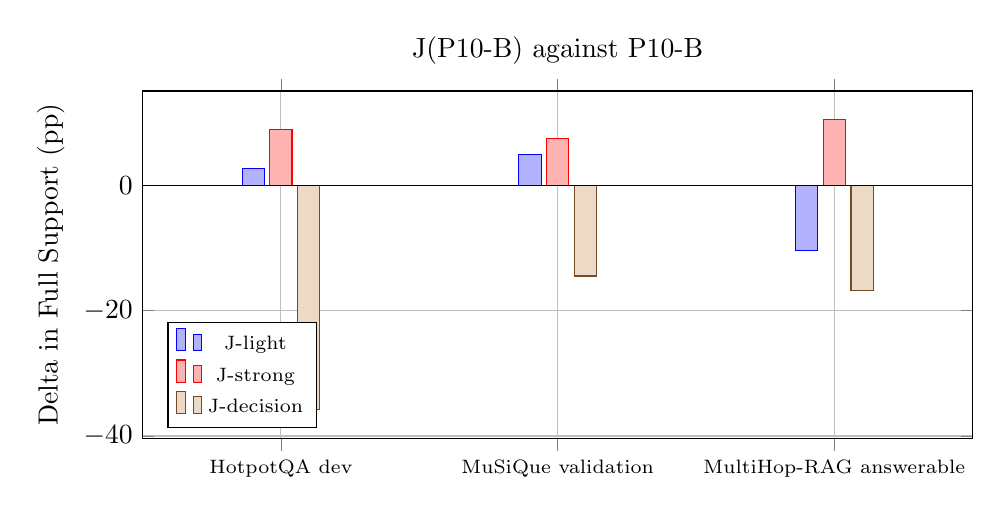
\begin{tikzpicture}
\begin{axis}[ybar, width=\columnwidth, height=6cm, bar width=8pt, enlarge x limits=0.25, xtick={0,1,2}, xticklabels={{HotpotQA dev},{MuSiQue validation},{MultiHop-RAG answerable}}, x tick label style={font=\scriptsize}, ylabel={Delta in Full Support (pp)}, grid=major, legend pos=south west, legend style={font=\scriptsize}, title={J(P10-B) against P10-B}]
\addplot coordinates {(0,2.62) (1,4.96) (2,-10.42)};
\addlegendentry{J-light}
\addplot coordinates {(0,8.94) (1,7.45) (2,10.42)};
\addlegendentry{J-strong}
\addplot coordinates {(0,-35.84) (1,-14.48) (2,-16.81)};
\addlegendentry{J-decision}
\draw (axis cs:-1,0) -- (axis cs:3,0);
\end{axis}
\end{tikzpicture}

\caption{Change in \FS{} when each judge reorders the standard recipe P10-B, in percentage
points, per set. Written from the artifacts.}
\label{fig:delta}
\end{figure}

\paragraph{The bi-encoder decision judge hurts everywhere: a negative result.} J-decision
lowers every system on every set, P10-B by \deltaDecisionPTenBHotpot\pp{} on HotpotQA,
\deltaDecisionPTenBMusique\pp{} on MuSiQue and \deltaDecisionPTenBMultihop\pp{} on news
(Figure~\ref{fig:delta}); J-decision(P10-B) wins \winsCrossDecisionVsStrongHotpot{} questions and loses
\lossesCrossDecisionVsStrongHotpot{} against J-strong(P10-B) on HotpotQA. Its hop labels are
\texttt{\labelDecisionHotpot}, \texttt{\labelDecisionMusique} and \texttt{\labelDecisionMultihop},
which are small differences between two bad orders. We read this as a measurement of this
\emph{use} of the model, not of the model: it is a bi-encoder that compares two separate
embeddings and cannot weigh a candidate's words against the question's the way a cross-encoder
does; it was designed for agent decisions, has no published passage-retrieval benchmark, and was
used here zero-shot with the question alone as its state and no instruction. We cannot separate
``it does not rank evidence'' from ``this usage does not suit it'', and the preregistration forbade
trying another prompt.

\paragraph{Determinism.} The two cross-encoders are deterministic to float noise: re-scoring
\detQuestionsLightHotpot{} questions at batch size one changed the order of \detOrderChangedLightHotpot{} of them,
with a largest score difference of \detMaxDiffLightHotpot{} for J-light and \detMaxDiffStrongHotpot{} for
J-strong on HotpotQA. J-decision is not: its encoder runs in bfloat16 (a 24~GB card cannot hold
it in float32) and the serving engine batches sequences itself, so the same re-scoring changed the order of
\detOrderChangedDecisionHotpot{} of \detQuestionsDecisionHotpot{} questions, with a largest difference of \detMaxDiffDecisionHotpot{} in the
score. Its figures are therefore one realization of the model; we did not measure how much a
second pass would move \FS, so the size of that effect is unknown.

\begin{figure}[t]
\centering
% Generated by `cer p17-tables`; do not edit. Coordinates are written from the artifacts.
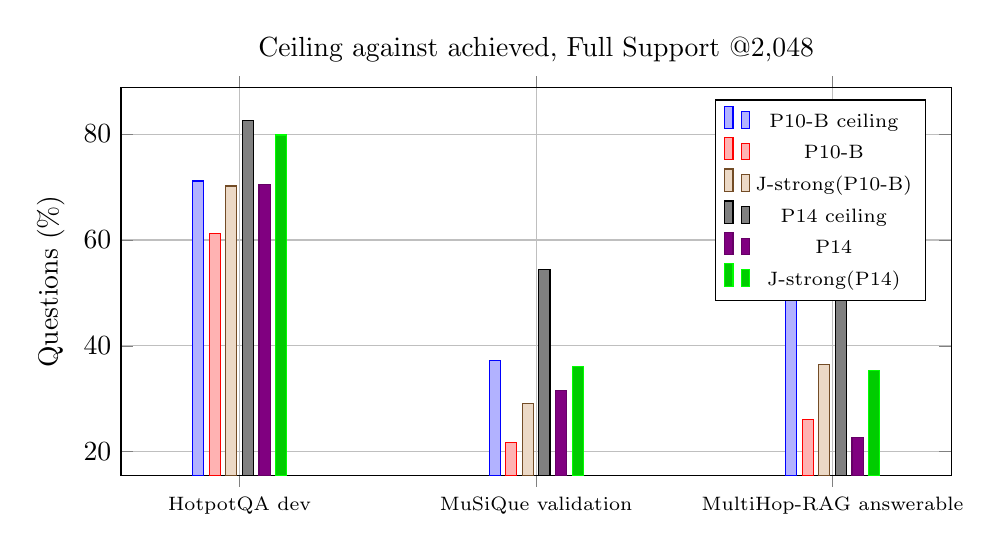
\begin{tikzpicture}
\begin{axis}[ybar, width=\columnwidth, height=6.5cm, bar width=4pt, enlarge x limits=0.2, xtick={0,1,2}, xticklabels={{HotpotQA dev},{MuSiQue validation},{MultiHop-RAG answerable}}, x tick label style={font=\scriptsize}, ylabel={Questions (\%)}, grid=major, legend pos=north east, legend style={font=\scriptsize}, title={Ceiling against achieved, Full Support @2,048}]
\addplot coordinates {(0,71.13) (1,37.24) (2,51.44)};
\addlegendentry{P10-B ceiling}
\addplot coordinates {(0,61.26) (1,21.68) (2,26.03)};
\addlegendentry{P10-B}
\addplot coordinates {(0,70.20) (1,29.13) (2,36.45)};
\addlegendentry{J-strong(P10-B)}
\addplot coordinates {(0,82.63) (1,54.49) (2,50.78)};
\addlegendentry{P14 ceiling}
\addplot coordinates {(0,70.55) (1,31.49) (2,22.75)};
\addlegendentry{P14}
\addplot coordinates {(0,79.82) (1,36.04) (2,35.34)};
\addlegendentry{J-strong(P14)}
\end{axis}
\end{tikzpicture}

\caption{The judge ceiling for the standard recipe and for P14: the share of questions whose
gold paragraphs all lie inside the system's top-100, beside what \FS{} the system achieves
without a judge and under J-strong.}
\label{fig:ceiling}
\end{figure}

\paragraph{How much of the room does a judge close?} A reorder cannot recover gold that lies outside the
pool; Figure~\ref{fig:ceiling} shows how far each system is from that bound. On HotpotQA, J-strong takes P10-B
from \fsPctPTenBHotpot{} to \fsPctStrongPTenBHotpot{} against a ceiling of
\ceilPTenBHotpot{} questions, and P14 to \fsPctStrongPFourteenHotpot{} (\fsStrongPFourteenHotpot{} questions
against a ceiling of \ceilPFourteenHotpot{}), only \ceilFailStrongPFourteenHotpot{} questions short of what its pool
allows. The union pool under J-strong reaches \fsStrongUnionHotpot{} questions: \textbf{P14 under J-strong
is at the union pool's level on HotpotQA}, so the hop's pool is already the best pool of the four there. On
MuSiQue P14's pool is the bigger one (a ceiling of \ceilPFourteenMusique{} against \ceilPTenBMusique{} for
P10-B), and under J-strong it reaches \fsStrongPFourteenMusique{} questions against \fsStrongUnionMusique{}
for the whole union pool; a hypothesis is that a larger pool lets a judge be wrong more often. On news P10-B's own pool
holds the gold of more questions than P14's (\ceilPTenBMultihop{} against \ceilPFourteenMultihop{}),
the opposite of the Wikipedia sets, and the union pool under J-strong is the best
line there (\fsStrongUnionMultihop{} questions). The ceilings are exploratory diagnostics computed from the gold.
The budget curve (Appendix~\ref{app:more}) shows that under J-strong the first 512 tokens already carry
\fsBudgetFiveTwelveStrongPFourteenHotpot{}\% on HotpotQA for P14, against \fsBudgetFiveTwelvePFourteenHotpot{}\%
without a judge.

\paragraph{Cost beside every figure.}
\begin{table}[t]
\centering
\small
\caption{\capJudgeCost}
\label{tab:judgecost}
\coltable{tables/judge-cost}
\end{table}
Table~\ref{tab:judgecost} gives pairs, throughput and attributable cost on one rented RTX~4090. J-light
scored all of HotpotQA's pairs in \wallSecLightHotpot{} s for \usdLightHotpot{} USD; J-strong took
\wallSecStrongHotpot{} s and \usdStrongHotpot{} USD; J-decision took \wallSecDecisionHotpot{} s and
\usdDecisionHotpot{} USD there. J-decision's wall time is dominated by embedding every distinct unit of
the pool once, which is why its pairs per second differ by an order of magnitude across the sets. The
three judges together cost \usdGpuAttributable{} USD of attributable GPU time; the whole rented session ran
\sessionHours{} h \sessionMinutes{} min and cost \usdSession{} USD by the balance recorded before and after
(derived). At query time a cross-encoder judge scores a pool of about \poolMeanHotpot{} pairs per
question on HotpotQA; the line's own systems, which call no model beyond the first Dense pass, are
never claimed to match a judge's quality at their cost.

\section{Published figures of other systems}
\label{sec:published}

Table~\ref{tab:published} lists \nPublishedRows{} figures published by other work on these
benchmarks: \nPublishedHotpotqa{} on HotpotQA, \nPublishedMusique{} on MuSiQue and \nPublishedMultihop{}
on MultiHop-RAG. They cover the BM25-plus-cross-encoder recipe and dense baselines of
BEIR~\citep{thakur2021beir}, trained multi-hop retrievers
(MDR~\citep{xiong2021mdr}, Baleen~\citep{khattab2021baleen}), retrieval interleaved with
language-model reasoning (IRCoT~\citep{trivedi2023ircot}, HippoRAG~\citep{gutierrez2024hipporag,gutierrez2025hipporag2})
and the MultiHop-RAG paper's own pipelines~\citep{tang2024multihoprag}. Each row was read in the
paper it comes from; \nPublishedExcluded{} candidate figures that could not be verified there were
excluded rather than quoted from a survey or another paper's table. The appendix repeats every row with its
corpus and a note on how it differs from our setting (Tables~\ref{tab:published-hotpotqa}
to~\ref{tab:published-multihop}).

\begin{table*}[!t]
\centering
\scriptsize
\setlength{\tabcolsep}{3pt}
\caption{\capPublishedShort}
\label{tab:published}
% Generated by `cer p17-tables`; do not edit.
% caption: Published figures of other systems on the three benchmarks, not a paired comparison with ours. Each row was read in the paper itself; the metric and the unit are the paper's own, and how each differs from our setting is in the appendix.
\begin{tabular}{p{5.2cm}p{6.4cm}rrp{2.1cm}l}
\toprule
System & Metric & Value & Questions & Training or LLM & Source \\
\midrule
\multicolumn{6}{l}{\textbf{HotpotQA}} \\
BM25 & nDCG@10 & 0.603 & 7,405 & none & \cite{thakur2021beir} \\
BM25 + cross-encoder reranking (MiniLM-L6, top-100) & nDCG@10 & 0.707 & 7,405 & trained retriever & \cite{thakur2021beir} \\
DPR & nDCG@10 & 0.391 & 7,405 & trained retriever & \cite{thakur2021beir} \\
ANCE & nDCG@10 & 0.456 & 7,405 & trained retriever & \cite{thakur2021beir} \\
TAS-B & nDCG@10 & 0.584 & 7,405 & trained retriever & \cite{thakur2021beir} \\
ColBERT (late interaction, end-to-end) & nDCG@10 & 0.593 & 7,405 & trained retriever & \cite{thakur2021beir} \\
MDR (multi-hop dense retriever, trained on HotpotQA) & R@2 (recall at k retrieved passages, percent) & 65.9 & -- & trained retriever & \cite{xiong2021mdr} \\
MDR (multi-hop dense retriever, trained on HotpotQA) & R@10 (recall at k retrieved passages, percent) & 77.5 & -- & trained retriever & \cite{xiong2021mdr} \\
MDR (multi-hop dense retriever, trained on HotpotQA) & R@20 (recall at k retrieved passages, percent) & 80.2 & -- & trained retriever & \cite{xiong2021mdr} \\
Baleen (FLIPR + condenser, trained on HotpotQA) & P-EM (both gold passages exactly selected, percent) & 86.7 & 7,405 & trained retriever & \cite{khattab2021baleen} \\
Baleen (FLIPR + condenser, trained on HotpotQA) & P-R@20 (top-20 passages contain both gold passages, percent) & 93.3 & 7,405 & trained retriever & \cite{khattab2021baleen} \\
BM25 & passage recall@2 (percent) on HotpotQA & 55.4 & 1,000 & none & \cite{gutierrez2024hipporag} \\
BM25 & passage recall@5 (percent) on HotpotQA & 72.2 & 1,000 & none & \cite{gutierrez2024hipporag} \\
ColBERTv2 & passage recall@2 (percent) on HotpotQA & 64.7 & 1,000 & trained retriever & \cite{gutierrez2024hipporag} \\
ColBERTv2 & passage recall@5 (percent) on HotpotQA & 79.3 & 1,000 & trained retriever & \cite{gutierrez2024hipporag} \\
HippoRAG (ColBERTv2) & passage recall@2 (percent) on HotpotQA & 60.5 & 1,000 & LLM in the loop & \cite{gutierrez2024hipporag} \\
HippoRAG (ColBERTv2) & passage recall@5 (percent) on HotpotQA & 77.7 & 1,000 & LLM in the loop & \cite{gutierrez2024hipporag} \\
IRCoT + ColBERTv2 & passage recall@2 (percent) on HotpotQA & 67.9 & 1,000 & LLM in the loop & \cite{gutierrez2024hipporag} \\
IRCoT + ColBERTv2 & passage recall@5 (percent) on HotpotQA & 82 & 1,000 & LLM in the loop & \cite{gutierrez2024hipporag} \\
IRCoT + HippoRAG (ColBERTv2) & passage recall@2 (percent) on HotpotQA & 67 & 1,000 & LLM in the loop & \cite{gutierrez2024hipporag} \\
IRCoT + HippoRAG (ColBERTv2) & passage recall@5 (percent) on HotpotQA & 83 & 1,000 & LLM in the loop & \cite{gutierrez2024hipporag} \\
BM25 & passage recall@2 (percent) on HotpotQA & 57.3 & 1,000 & none & \cite{gutierrez2025hipporag2} \\
BM25 & passage recall@5 (percent) on HotpotQA & 74.8 & 1,000 & none & \cite{gutierrez2025hipporag2} \\
NV-Embed-v2 (7B dense retriever) & passage recall@2 (percent) on HotpotQA & 84.1 & 1,000 & trained retriever & \cite{gutierrez2025hipporag2} \\
NV-Embed-v2 (7B dense retriever) & passage recall@5 (percent) on HotpotQA & 94.5 & 1,000 & trained retriever & \cite{gutierrez2025hipporag2} \\
HippoRAG 2 (Llama-3.3-70B-Instruct) & passage recall@2 (percent) on HotpotQA & 83.5 & 1,000 & LLM in the loop & \cite{gutierrez2025hipporag2} \\
HippoRAG 2 (Llama-3.3-70B-Instruct) & passage recall@5 (percent) on HotpotQA & 96.3 & 1,000 & LLM in the loop & \cite{gutierrez2025hipporag2} \\
\midrule
\multicolumn{6}{l}{\textbf{MuSiQue}} \\
BM25 & passage recall@2 (percent) on MuSiQue (answerable) & 32.3 & 1,000 & none & \cite{gutierrez2024hipporag} \\
BM25 & passage recall@5 (percent) on MuSiQue (answerable) & 41.2 & 1,000 & none & \cite{gutierrez2024hipporag} \\
ColBERTv2 & passage recall@2 (percent) on MuSiQue (answerable) & 37.9 & 1,000 & trained retriever & \cite{gutierrez2024hipporag} \\
ColBERTv2 & passage recall@5 (percent) on MuSiQue (answerable) & 49.2 & 1,000 & trained retriever & \cite{gutierrez2024hipporag} \\
HippoRAG (ColBERTv2) & passage recall@2 (percent) on MuSiQue (answerable) & 40.9 & 1,000 & LLM in the loop & \cite{gutierrez2024hipporag} \\
HippoRAG (ColBERTv2) & passage recall@5 (percent) on MuSiQue (answerable) & 51.9 & 1,000 & LLM in the loop & \cite{gutierrez2024hipporag} \\
IRCoT + ColBERTv2 & passage recall@2 (percent) on MuSiQue (answerable) & 41.7 & 1,000 & LLM in the loop & \cite{gutierrez2024hipporag} \\
IRCoT + ColBERTv2 & passage recall@5 (percent) on MuSiQue (answerable) & 53.7 & 1,000 & LLM in the loop & \cite{gutierrez2024hipporag} \\
IRCoT + HippoRAG (ColBERTv2) & passage recall@2 (percent) on MuSiQue (answerable) & 45.3 & 1,000 & LLM in the loop & \cite{gutierrez2024hipporag} \\
IRCoT + HippoRAG (ColBERTv2) & passage recall@5 (percent) on MuSiQue (answerable) & 57.6 & 1,000 & LLM in the loop & \cite{gutierrez2024hipporag} \\
BM25 & passage recall@2 (percent) on MuSiQue & 32.4 & 1,000 & none & \cite{gutierrez2025hipporag2} \\
BM25 & passage recall@5 (percent) on MuSiQue & 43.5 & 1,000 & none & \cite{gutierrez2025hipporag2} \\
NV-Embed-v2 (7B dense retriever) & passage recall@2 (percent) on MuSiQue & 52.7 & 1,000 & trained retriever & \cite{gutierrez2025hipporag2} \\
NV-Embed-v2 (7B dense retriever) & passage recall@5 (percent) on MuSiQue & 69.7 & 1,000 & trained retriever & \cite{gutierrez2025hipporag2} \\
HippoRAG 2 (Llama-3.3-70B-Instruct) & passage recall@2 (percent) on MuSiQue & 56.1 & 1,000 & LLM in the loop & \cite{gutierrez2025hipporag2} \\
HippoRAG 2 (Llama-3.3-70B-Instruct) & passage recall@5 (percent) on MuSiQue & 74.7 & 1,000 & LLM in the loop & \cite{gutierrez2025hipporag2} \\
\midrule
\multicolumn{6}{l}{\textbf{MultiHop-RAG}} \\
text-embedding-ada-002 (without reranker) & Hits@10 & 0.6381 & 2,255 & trained retriever & \cite{tang2024multihoprag} \\
text-embedding-ada-002 (without reranker) & Hits@4 & 0.504 & 2,255 & trained retriever & \cite{tang2024multihoprag} \\
text-embedding-ada-002 (with bge-reranker-large) & Hits@10 & 0.7059 & 2,255 & trained retriever & \cite{tang2024multihoprag} \\
text-embedding-ada-002 (with bge-reranker-large) & Hits@4 & 0.6169 & 2,255 & trained retriever & \cite{tang2024multihoprag} \\
bge-large-en-v1.5 (without reranker) & Hits@10 & 0.6718 & 2,255 & trained retriever & \cite{tang2024multihoprag} \\
bge-large-en-v1.5 (without reranker) & Hits@4 & 0.5221 & 2,255 & trained retriever & \cite{tang2024multihoprag} \\
bge-large-en-v1.5 (with bge-reranker-large) & Hits@10 & 0.7183 & 2,255 & trained retriever & \cite{tang2024multihoprag} \\
bge-large-en-v1.5 (with bge-reranker-large) & Hits@4 & 0.6364 & 2,255 & trained retriever & \cite{tang2024multihoprag} \\
voyage-02 (without reranker) & Hits@10 & 0.6506 & 2,255 & trained retriever & \cite{tang2024multihoprag} \\
voyage-02 (without reranker) & Hits@4 & 0.4619 & 2,255 & trained retriever & \cite{tang2024multihoprag} \\
voyage-02 (with bge-reranker-large) & Hits@10 & 0.7467 & 2,255 & trained retriever & \cite{tang2024multihoprag} \\
voyage-02 (with bge-reranker-large) & Hits@4 & 0.6625 & 2,255 & trained retriever & \cite{tang2024multihoprag} \\
\bottomrule
\end{tabular}

\end{table*}

\paragraph{What the reader may conclude.} Our nDCG@10 and gold-recall figures
(Appendix~\ref{app:d6}) use the corpus unit, the whole paragraph, and the same questions
and corpus as BEIR on HotpotQA, so they can be laid beside the BM25-plus-cross-encoder row as
context: for instance, our J-light over Dense plus BM25 reaches \ndcgLightPTenBHotpot{} (nDCG@10, times
one hundred), and J-strong \ndcgStrongPTenBHotpot{}. They place the zero-shot recipe of this paper in the
same range as other zero-shot recipes on identical questions.

\paragraph{What the reader may not conclude.} These are \emph{published figures, not a paired
comparison}. The rows differ from our setting in at least one of the unit of retrieval
(chunks of a fixed token length, or whole paragraphs), the metric (nDCG with graded relevance, recall at
a rank, hits at a rank, or our token-budget Full Support), the corpus (a pooled
corpus of a subset of questions, or the whole of Wikipedia), the questions (a sampled subset, or all of
them), and whether the system is trained or calls a language model; the differences column says which,
row by row. Our weights are fitted on HotpotQA development questions, so our HotpotQA figures are
in-sample for P10-C and P14. Our systems are untrained, call no model at query time, and are
cheap; they are not offered as competitors of trained or language-model-based systems, and
nothing in this paper shows that they match or beat those systems.

\section{The concept-space negative result}
\label{sec:concepts}

The line began with a different structure. Phases 2 to 4 asked whether a \emph{concept space}
induced from pooled Dense embeddings (a dictionary learned from the embeddings by sparse dictionary learning, with
each paragraph coded as a sparse non-negative combination of its concepts) could guide retrieval toward the missing paragraph of a multi-hop question. It could
not. Concepts added nothing over Dense; a Dense plus BM25 control, added as a fair comparator,
beat them; and a diffusion step over the concept space re-ranked what was already retrieved
without promoting a new paragraph. The line was closed with a bounded negative result.
A later phase tried concepts \emph{read from the text} and found that entities help the hop
while the text-derived concepts were the weakest hop measured and made entities worse when added.
The negative result is bounded to those two operationalizations on this benchmark; it is not
evidence against text-derived entities, which is what the rest of the paper uses.

\section{Limitations}
\label{sec:limits}

\begin{enumerate}
  \item \textbf{The judges are zero-shot models with their own training domain.} The two
        cross-encoders are zero-shot models trained on English web question answering
        (MS~MARCO); CLM-8B on question-answer pairs, synthetic hard negatives and agentic
        trajectories. Their behaviour on news, on MuSiQue's composed
        questions and on HotpotQA is itself a transfer, and no domain adaptation was attempted.
  \item \textbf{The pool is bounded at the first hundred.} Gold outside every system's top-100
        is unreachable by any reorder: on MuSiQue and MultiHop-RAG only \ceilUnionMusique{} of
        \nQuestionsMusique{} and \ceilUnionMultihop{} of \nQuestionsMultihop{} questions have every gold unit
        in the union pool. The judge results bound what better \emph{ordering} can give, not what
        better retrieval could (the ceiling table is in Appendix~\ref{app:more}).
  \item \textbf{HotpotQA development questions are in-sample for P10-C's and P14's weights.}
        The judge figures on that set are still informative because the judges are fitted on
        nothing, but the HotpotQA columns for those two systems are not held out. BGE-small was
        also fine-tuned on HotpotQA training questions, which the held-out draws of earlier phases
        use.
  \item \textbf{One-hop design, two- to four-paragraph questions.} The hop anchors on the first
        Dense paragraph and follows one hop. The gain is on questions with two supporting
        paragraphs and absent on four; on news the first paragraph is rarely gold, and the design
        fails there.
  \item \textbf{Corpus sizes and kinds.} Only HotpotQA is measured at the scale of the full
        Wikipedia (\hopCostNineUnits{} paragraphs). MuSiQue is \hopCostFifteenUnits{} paragraphs and
        MultiHop-RAG \hopCostSixteenUnits{}: the transfer evidence is two small pools, one of
        Wikipedia and one of news. No stronger Dense retriever than BGE-small was tested beside
        the hop.
  \item \textbf{MultiHop-RAG's queries were written by a language model} from the articles, so
        their wording may favour lexical overlap with the evidence; that is one candidate
        reason BM25 gives the largest step there, and we did not test it.
  \item \textbf{The metric of record packs whole paragraphs into a token budget}, and the
        comparable metrics count units. Neither equals a chunk-level metric of a paper that cut
        its corpus differently (Section~\ref{sec:published}).
  \item \textbf{The cost of a judge is real at query time.} A judge scores a pool of
        candidates per question; the paper reports pairs per second and dollars beside every
        figure, and the line's systems are never claimed to match a judge's quality at their cost.
  \item \textbf{A bi-encoder judge does not read the question and the candidate together.}
        J-decision compares two separate embeddings, and CLM-8B has no published passage-retrieval
        benchmark, so what this paper measures is whether it judges evidence well, not an
        assumption that it does. Its bfloat16 encoder is also not deterministic under batching
        (Section~\ref{sec:judges}): its figures are one realization, and we did not measure how far
        another pass would move them.
  \item \textbf{A paper is a claim under review.} It reports what one author, with AI assistance,
        measured on public benchmarks; the artifacts and the code are public so that each figure
        can be checked, and whether it is accepted anywhere is outside this work.
\end{enumerate}

\section{Conclusion and what comes next}
\label{sec:conclusion}

A query-blind, one-hop entity signal, read once by a cheap zero-shot extractor, recovers a share of
the multi-hop evidence Dense misses and adds to Dense plus BM25 at full HotpotQA scale and, with
nothing refitted, on MuSiQue. It does not transfer to news, and we do not know the boundary of
where it does. Placed beside a zero-shot cross-encoder, the control the line was missing, the
picture is more mixed than the earlier phases suggested: a strong judge lifts every system on every
corpus; the hop's candidates still add under it on the two Wikipedia benchmarks and do not on news;
a bi-encoder decision model hurts everywhere, which reads as a limit of that use of the model and
leaves its quality as evidence judge open. Under the strong judge P14 remains the best of the
four systems on HotpotQA (\fsStrongPFourteenHotpot{} questions, at the level of the union pool
of all four candidate lists, \fsStrongUnionHotpot{}) and on MuSiQue
(\fsStrongPFourteenMusique{}); on news the judged Dense plus BM25 leads
(\fsStrongPTenBMultihop{} against \fsStrongPFourteenMultihop{}). The size of a judge is not
what decides: the strong cross-encoder is a fraction of the decision model's parameters and
reads the question and the candidate together, which the decision model does not.

Two readings follow, both stated as hypotheses supported on Wikipedia and not on news. First,
under a judge the hop's role is \emph{candidate generation}: its value is in what it adds to the
pool, not in its own ordering. Second, the union pool under a judge is the natural reference for
the next project, because it is the best pool any of these systems can offer and what a better
orderer would be measured against. The successor project takes both: a judge-ordered union pool as
the reference, and the Entity Hop as one candidate generator among others, with its
indexing and query cost reported beside every result as here.


\ifanonymous\else
\section*{Acknowledgements}
Code, analysis and drafting were produced with AI assistance (Claude); the author designed the
experiments, approved every specification and plan, and is responsible for the content. The
repository is at \repourl.
\fi

\bibliographystyle{plainnat}
\bibliography{references}

\appendix
\section{Reproducibility}
\label{app:repro}

\paragraph{Artifacts.} Every table, plot and number in the paper is written by
\texttt{uv run cer p17-tables} from the committed artifacts of Phase~17 (\texttt{data/phase17/}) and,
read-only, the outcome files of Phases~9, 10, 14, 15 and~16. The generated files are committed under
\texttt{docs/paper/tables} and \texttt{docs/paper/figures}; each macro in \texttt{numbers.tex}
carries its artifact path, the SHA-256 prefix of that file and the JSON key it was read from.
Table~\ref{tab:sha} gives the full SHA-256 of the files the text cites; the Phase~9, 10 and 14 outcome files are
not in git, so their digests are the record.

\begin{table*}[t]
\centering
\scriptsize
\caption{SHA-256 of the artifacts the paper reads (written from the files by the generator).}
\label{tab:sha}
\begin{tabular}{ll}
\toprule
Artifact & SHA-256 \\
\midrule
\texttt{data/phase17/outcome.json} & \texttt{\shaOutcome} \\
\texttt{data/phase17/metrics.json} & \texttt{\shaMetrics} \\
\texttt{data/phase17/pool.json} & \texttt{\shaPool} \\
\texttt{data/phase17/integrity.json} & \texttt{\shaIntegrity} \\
\texttt{data/phase17/scoring-light.json} & \texttt{\shaScoringLight} \\
\texttt{data/phase17/scoring-strong.json} & \texttt{\shaScoringStrong} \\
\texttt{data/phase17/scoring-decision.json} & \texttt{\shaScoringDecision} \\
\texttt{data/phase17/published-figures.json} & \texttt{\shaPublished} \\
\texttt{data/phase9/outcome.json} & \texttt{\shaPhaseNineOutcome} \\
\texttt{data/phase10/outcome.json} & \texttt{\shaPhaseTenOutcome} \\
\texttt{data/phase14/outcome.json} & \texttt{\shaPhaseFourteenOutcome} \\
\texttt{data/phase15/outcome.json} & \texttt{\shaPhaseFifteenOutcome} \\
\texttt{data/phase16/outcome.json} & \texttt{\shaPhaseSixteenOutcome} \\
\bottomrule
\end{tabular}
\end{table*}

\paragraph{Pins.} Table~\ref{tab:judges} gives each judge's model, revision, parameters, maximum
length and precision; each scoring manifest also records the library versions, the code commit,
the weights' SHA-256 and the serving command. The extractor is GLiNER
GLiNER (the medium zero-shot model) at a pinned revision recorded in the repository's
configuration, and the Dense model is BGE-small at a pinned revision. Seeds are explicit and ties are broken by a deterministic rule.

\paragraph{The rented session.} All scoring ran in one session on a rented RTX~4090 at
\judgeRateLight{} USD per hour, driven over SSH from the laptop: \sessionHours{} h \sessionMinutes{} min, a balance
drop of \usdSession{} USD, of which \usdGpuAttributable{} USD is attributable to scoring (derived from
measured time and the hourly rate; Table~\ref{tab:judgecost}). Nothing else ran on a GPU in this
phase; the paper itself builds on a laptop.

\paragraph{Build.} \texttt{uv run python docs/paper/build.py} regenerates the tables, runs Tectonic
on \texttt{docs/paper/main.tex}, and prints the page count and the SHA-256 of the PDF. The
\texttt{\textbackslash anonymoustrue} switch in \texttt{main.tex} drops the author, the repository
URL and the acknowledgements for double-blind review. The R5 guard
(\texttt{paper.r5\_violations}) runs inside \texttt{cer p17-tables} and refuses any hand-written
number with a decimal point, a thousands separator or a percent sign.

\section{Paired comparisons (D5)}
\label{app:d5}

\begin{table*}[t]
\centering
\scriptsize
\caption{\capDFiveHotpotqa}
% Generated by `cer p17-tables`; do not edit.
% caption: HotpotQA dev, 7,405 questions: the paired comparisons of D5 (exact two-sided McNemar on Full Support); the label is that of J(P14) against J(P10-B).
\begin{tabular}{lrrrrrl}
\toprule
Comparison & Wins & Losses & Ties & Delta (pp) & p & Label \\
\midrule
J-light(P10-A) vs P10-A & 665 & 228 & 6,512 & +5.90 & $3.0\times10^{-50}$ &  \\
J-light(P10-B) vs P10-B & 445 & 251 & 6,709 & +2.62 & $1.8\times10^{-13}$ &  \\
J-light(P10-C) vs P10-C & 524 & 411 & 6,470 & +1.53 & $2.5\times10^{-4}$ &  \\
J-light(P14) vs J-light(P10-B) & 383 & 59 & 6,963 & +4.38 & $3.1\times10^{-59}$ & HOP\_ADDS\_UNDER\_JUDGE \\
J-light(P14) vs P14 & 441 & 611 & 6,353 & $-$2.30 & $1.8\times10^{-7}$ &  \\
\midrule
J-strong(P10-A) vs P10-A & 875 & 36 & 6,494 & +11.33 & $5.6\times10^{-210}$ &  \\
J-strong(P10-B) vs P10-B & 685 & 23 & 6,697 & +8.94 & $1.5\times10^{-170}$ &  \\
J-strong(P10-C) vs P10-C & 846 & 78 & 6,481 & +10.37 & $1.0\times10^{-163}$ &  \\
J-strong(P14) vs J-strong(P10-B) & 780 & 67 & 6,558 & +9.63 & $6.4\times10^{-155}$ & HOP\_ADDS\_UNDER\_JUDGE \\
J-strong(P14) vs P14 & 798 & 111 & 6,496 & +9.28 & $6.9\times10^{-129}$ &  \\
\midrule
J-decision(P10-A) vs P10-A & 182 & 2,749 & 4,474 & $-$34.67 & $<10^{-300}$ &  \\
J-decision(P10-B) vs P10-B & 148 & 2,802 & 4,455 & $-$35.84 & $<10^{-300}$ &  \\
J-decision(P10-C) vs P10-C & 194 & 3,012 & 4,199 & $-$38.06 & $<10^{-300}$ &  \\
J-decision(P14) vs J-decision(P10-B) & 264 & 256 & 6,885 & +0.11 & $7.6\times10^{-1}$ & HOP\_NEUTRAL\_UNDER\_JUDGE \\
J-decision(P14) vs P14 & 155 & 3,489 & 3,761 & $-$45.02 & $<10^{-300}$ &  \\
\midrule
J-decision(P10-B) vs J-strong(P10-B) & 12 & 3,328 & 4,065 & $-$44.78 & $<10^{-300}$ &  \\
J-strong(P10-B) vs J-light(P10-B) & 494 & 26 & 6,885 & +6.32 & $3.3\times10^{-113}$ &  \\
\bottomrule
\end{tabular}

\end{table*}

\begin{table*}[t]
\centering
\scriptsize
\caption{\capDFiveMusique}
% Generated by `cer p17-tables`; do not edit.
% caption: MuSiQue validation, 2,417 questions: the paired comparisons of D5 (exact two-sided McNemar on Full Support); the label is that of J(P14) against J(P10-B).
\begin{tabular}{lrrrrrl}
\toprule
Comparison & Wins & Losses & Ties & Delta (pp) & p & Label \\
\midrule
J-light(P10-A) vs P10-A & 201 & 42 & 2,174 & +6.58 & $4.6\times10^{-26}$ &  \\
J-light(P10-B) vs P10-B & 176 & 56 & 2,185 & +4.96 & $1.2\times10^{-15}$ &  \\
J-light(P10-C) vs P10-C & 173 & 172 & 2,072 & +0.04 & $1.0\times10^{0}$ &  \\
J-light(P14) vs J-light(P10-B) & 68 & 15 & 2,334 & +2.19 & $3.2\times10^{-9}$ & HOP\_ADDS\_UNDER\_JUDGE \\
J-light(P14) vs P14 & 172 & 236 & 2,009 & $-$2.65 & $1.8\times10^{-3}$ &  \\
\midrule
J-strong(P10-A) vs P10-A & 247 & 41 & 2,129 & +8.52 & $4.9\times10^{-37}$ &  \\
J-strong(P10-B) vs P10-B & 230 & 50 & 2,137 & +7.45 & $9.3\times10^{-29}$ &  \\
J-strong(P10-C) vs P10-C & 261 & 126 & 2,030 & +5.59 & $5.9\times10^{-12}$ &  \\
J-strong(P14) vs J-strong(P10-B) & 190 & 23 & 2,204 & +6.91 & $7.0\times10^{-34}$ & HOP\_ADDS\_UNDER\_JUDGE \\
J-strong(P14) vs P14 & 272 & 162 & 1,983 & +4.55 & $1.4\times10^{-7}$ &  \\
\midrule
J-decision(P10-A) vs P10-A & 56 & 337 & 2,024 & $-$11.63 & $5.3\times10^{-50}$ &  \\
J-decision(P10-B) vs P10-B & 47 & 397 & 1,973 & $-$14.48 & $4.1\times10^{-70}$ &  \\
J-decision(P10-C) vs P10-C & 56 & 504 & 1,857 & $-$18.54 & $3.9\times10^{-91}$ &  \\
J-decision(P14) vs J-decision(P10-B) & 70 & 22 & 2,325 & +1.99 & $5.3\times10^{-7}$ & HOP\_ADDS\_UNDER\_JUDGE \\
J-decision(P14) vs P14 & 42 & 581 & 1,794 & $-$22.30 & $2.5\times10^{-122}$ &  \\
\midrule
J-decision(P10-B) vs J-strong(P10-B) & 22 & 552 & 1,843 & $-$21.93 & $9.9\times10^{-134}$ &  \\
J-strong(P10-B) vs J-light(P10-B) & 121 & 61 & 2,235 & +2.48 & $1.0\times10^{-5}$ &  \\
\bottomrule
\end{tabular}

\end{table*}

\begin{table*}[t]
\centering
\scriptsize
\caption{\capDFiveMultihopRag}
% Generated by `cer p17-tables`; do not edit.
% caption: MultiHop-RAG answerable, 2,255 questions: the paired comparisons of D5 (exact two-sided McNemar on Full Support); the label is that of J(P14) against J(P10-B).
\begin{tabular}{lrrrrrl}
\toprule
Comparison & Wins & Losses & Ties & Delta (pp) & p & Label \\
\midrule
J-light(P10-A) vs P10-A & 124 & 152 & 1,979 & $-$1.24 & $1.0\times10^{-1}$ &  \\
J-light(P10-B) vs P10-B & 89 & 324 & 1,842 & $-$10.42 & $1.9\times10^{-32}$ &  \\
J-light(P10-C) vs P10-C & 105 & 283 & 1,867 & $-$7.89 & $5.6\times10^{-20}$ &  \\
J-light(P14) vs J-light(P10-B) & 14 & 27 & 2,214 & $-$0.58 & $6.0\times10^{-2}$ & HOP\_NEUTRAL\_UNDER\_JUDGE \\
J-light(P14) vs P14 & 98 & 272 & 1,885 & $-$7.72 & $4.7\times10^{-20}$ &  \\
\midrule
J-strong(P10-A) vs P10-A & 313 & 38 & 1,904 & +12.20 & $6.2\times10^{-55}$ &  \\
J-strong(P10-B) vs P10-B & 289 & 54 & 1,912 & +10.42 & $5.8\times10^{-40}$ &  \\
J-strong(P10-C) vs P10-C & 321 & 50 & 1,884 & +12.02 & $1.5\times10^{-49}$ &  \\
J-strong(P14) vs J-strong(P10-B) & 24 & 49 & 2,182 & $-$1.11 & $4.6\times10^{-3}$ & HOP\_HURTS\_UNDER\_JUDGE \\
J-strong(P14) vs P14 & 338 & 54 & 1,863 & +12.59 & $2.4\times10^{-51}$ &  \\
\midrule
J-decision(P10-A) vs P10-A & 80 & 251 & 1,924 & $-$7.58 & $1.1\times10^{-21}$ &  \\
J-decision(P10-B) vs P10-B & 60 & 439 & 1,756 & $-$16.81 & $3.2\times10^{-72}$ &  \\
J-decision(P10-C) vs P10-C & 59 & 407 & 1,789 & $-$15.43 & $5.2\times10^{-65}$ &  \\
J-decision(P14) vs J-decision(P10-B) & 21 & 44 & 2,190 & $-$1.02 & $5.9\times10^{-3}$ & HOP\_HURTS\_UNDER\_JUDGE \\
J-decision(P14) vs P14 & 71 & 399 & 1,785 & $-$14.55 & $1.9\times10^{-56}$ &  \\
\midrule
J-decision(P10-B) vs J-strong(P10-B) & 26 & 640 & 1,589 & $-$27.23 & $2.6\times10^{-154}$ &  \\
J-strong(P10-B) vs J-light(P10-B) & 511 & 41 & 1,703 & +20.84 & $2.5\times10^{-104}$ &  \\
\bottomrule
\end{tabular}

\end{table*}

\section{Comparable metrics (D6)}
\label{app:d6}

\begin{table*}[t]
\centering
\scriptsize
\caption{\capDSixHotpotqa}
\pagetable{tables/d6-hotpotqa}
\end{table*}

\begin{table*}[t]
\centering
\scriptsize
\caption{\capDSixMusique}
\pagetable{tables/d6-musique}
\end{table*}

\begin{table*}[t]
\centering
\scriptsize
\caption{\capDSixMultihopRag}
\pagetable{tables/d6-multihop-rag}
\end{table*}

\section{Budget curves and ceilings}
\label{app:more}

\begin{table}[t]
\centering
\scriptsize
\caption{\capBudgetCurve}
\coltable{tables/budget-curve}
\end{table}

\begin{figure}[t]
\centering
% Generated by `cer p17-tables`; do not edit. Coordinates are written from the artifacts.
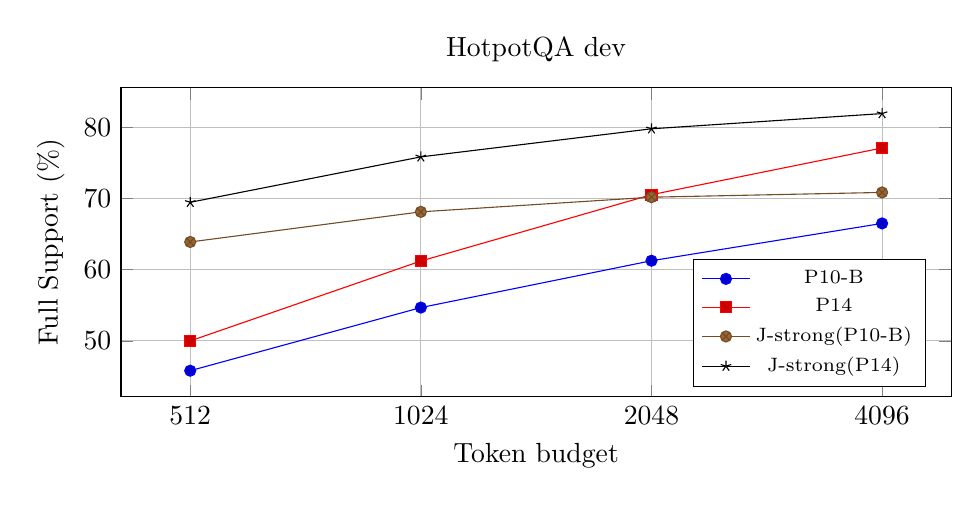
\begin{tikzpicture}
\begin{axis}[width=\columnwidth, height=5.5cm, xmode=log, log basis x=2, xtick={512,1024,2048,4096}, xticklabels={512,1024,2048,4096}, xlabel={Token budget}, ylabel={Full Support (\%)}, grid=major, legend pos=south east, legend style={font=\scriptsize}, title={HotpotQA dev}]
\addplot coordinates {(512,45.79) (1024,54.67) (2048,61.26) (4096,66.51)};
\addlegendentry{P10-B}
\addplot coordinates {(512,49.98) (1024,61.22) (2048,70.55) (4096,77.12)};
\addlegendentry{P14}
\addplot coordinates {(512,63.90) (1024,68.14) (2048,70.20) (4096,70.87)};
\addlegendentry{J-strong(P10-B)}
\addplot coordinates {(512,69.48) (1024,75.87) (2048,79.82) (4096,81.96)};
\addlegendentry{J-strong(P14)}
\end{axis}
\end{tikzpicture}

\caption{\FS{} against the token budget on HotpotQA development questions, for P10-B and P14
with and without J-strong.}
\end{figure}

\begin{figure}[t]
\centering
% Generated by `cer p17-tables`; do not edit. Coordinates are written from the artifacts.
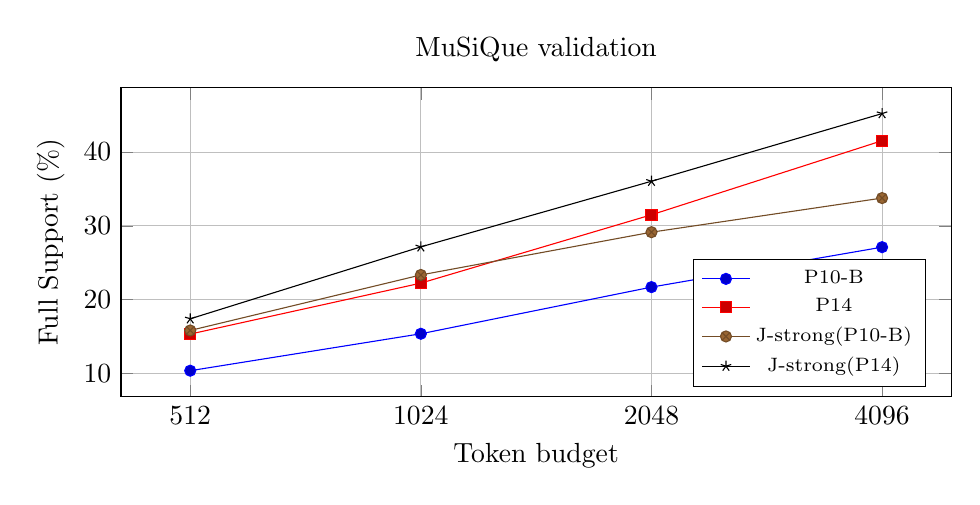
\begin{tikzpicture}
\begin{axis}[width=\columnwidth, height=5.5cm, xmode=log, log basis x=2, xtick={512,1024,2048,4096}, xticklabels={512,1024,2048,4096}, xlabel={Token budget}, ylabel={Full Support (\%)}, grid=major, legend pos=south east, legend style={font=\scriptsize}, title={MuSiQue validation}]
\addplot coordinates {(512,10.34) (1024,15.35) (2048,21.68) (4096,27.10)};
\addlegendentry{P10-B}
\addplot coordinates {(512,15.31) (1024,22.22) (2048,31.49) (4096,41.54)};
\addlegendentry{P14}
\addplot coordinates {(512,15.80) (1024,23.33) (2048,29.13) (4096,33.76)};
\addlegendentry{J-strong(P10-B)}
\addplot coordinates {(512,17.38) (1024,27.14) (2048,36.04) (4096,45.22)};
\addlegendentry{J-strong(P14)}
\end{axis}
\end{tikzpicture}

\caption{The same on MuSiQue validation.}
\end{figure}

\begin{figure}[t]
\centering
% Generated by `cer p17-tables`; do not edit. Coordinates are written from the artifacts.
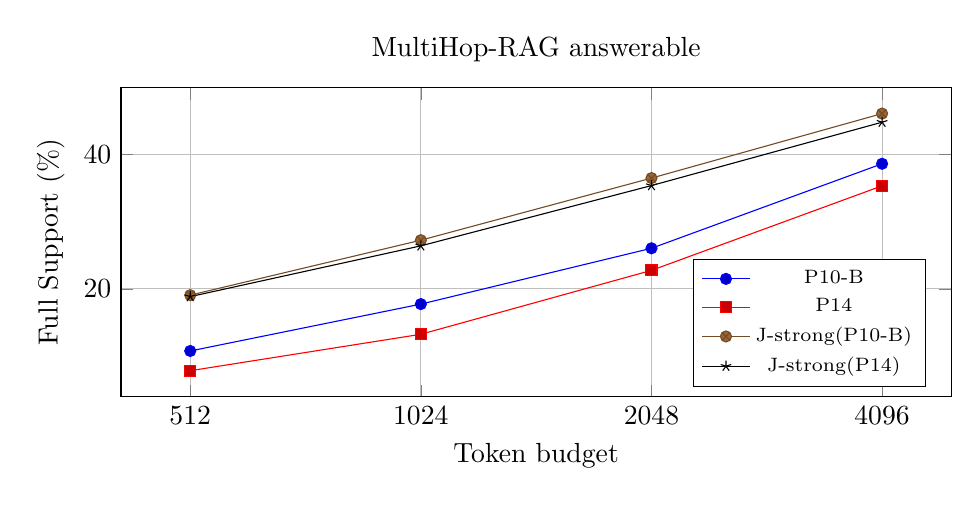
\begin{tikzpicture}
\begin{axis}[width=\columnwidth, height=5.5cm, xmode=log, log basis x=2, xtick={512,1024,2048,4096}, xticklabels={512,1024,2048,4096}, xlabel={Token budget}, ylabel={Full Support (\%)}, grid=major, legend pos=south east, legend style={font=\scriptsize}, title={MultiHop-RAG answerable}]
\addplot coordinates {(512,10.78) (1024,17.74) (2048,26.03) (4096,38.58)};
\addlegendentry{P10-B}
\addplot coordinates {(512,7.85) (1024,13.26) (2048,22.75) (4096,35.30)};
\addlegendentry{P14}
\addplot coordinates {(512,19.07) (1024,27.23) (2048,36.45) (4096,46.03)};
\addlegendentry{J-strong(P10-B)}
\addplot coordinates {(512,18.85) (1024,26.39) (2048,35.34) (4096,44.75)};
\addlegendentry{J-strong(P14)}
\end{axis}
\end{tikzpicture}

\caption{The same on MultiHop-RAG.}
\end{figure}

\begin{table*}[t]
\centering
\scriptsize
\caption{\capCeiling}
\pagetable{tables/ceiling}
\end{table*}

\clearpage
\onecolumn
\section{Published figures, row by row}
\label{app:pub}

\begingroup
\scriptsize
\setlength{\tabcolsep}{3pt}
% Generated by `cer p17-tables`; do not edit.
% caption: HotpotQA: published figures, not a paired comparison. Each row was read in the paper itself; the last column says what differs from our setting.
\begin{tabular}{p{2.4cm}p{2.0cm}rrp{2.6cm}p{1.6cm}p{5.2cm}l}
\toprule
System & Metric & Value & Questions & Corpus & Training or LLM & Differences from ours & Source \\
\midrule
BM25 & nDCG@10 & 0.603 & 7,405 & HotpotQA Wikipedia abstracts (BEIR cut) (5,233,329) & none & Same 7,405 questions and 5,233,329 paragraphs as our fullwiki setting, but the metric is nDCG@10 over graded-binary per-paragraph relevance, not Full Support @2,048 tokens nor paragraph-pair recall at k; the BEIR split is the official 7,405-question set, which we use as dev. Lexical, no training. & \cite{thakur2021beir} \\
BM25 + cross-encoder reranking (MiniLM-L6, top-100) & nDCG@10 & 0.707 & 7,405 & HotpotQA Wikipedia abstracts (BEIR cut) (5,233,329) & trained retriever & Same 7,405 questions and 5,233,329 paragraphs as our fullwiki setting, but the metric is nDCG@10 over graded-binary per-paragraph relevance, not Full Support @2,048 tokens nor paragraph-pair recall at k; the BEIR split is the official 7,405-question set, which we use as dev. First stage BM25 (Anserini), top-100 reranked by a 6-layer 384-d MiniLM cross-encoder trained on MS MARCO (zero-shot on HotpotQA); the closest published analogue of our J-light recipe, though our rerank depth and unit differ. & \cite{thakur2021beir} \\
DPR & nDCG@10 & 0.391 & 7,405 & HotpotQA Wikipedia abstracts (BEIR cut) (5,233,329) & trained retriever & Same 7,405 questions and 5,233,329 paragraphs as our fullwiki setting, but the metric is nDCG@10 over graded-binary per-paragraph relevance, not Full Support @2,048 tokens nor paragraph-pair recall at k; the BEIR split is the official 7,405-question set, which we use as dev. Trained on MS MARCO (BEIR re-trained it), zero-shot on HotpotQA. & \cite{thakur2021beir} \\
ANCE & nDCG@10 & 0.456 & 7,405 & HotpotQA Wikipedia abstracts (BEIR cut) (5,233,329) & trained retriever & Same 7,405 questions and 5,233,329 paragraphs as our fullwiki setting, but the metric is nDCG@10 over graded-binary per-paragraph relevance, not Full Support @2,048 tokens nor paragraph-pair recall at k; the BEIR split is the official 7,405-question set, which we use as dev. Trained on MS MARCO, zero-shot on HotpotQA. & \cite{thakur2021beir} \\
TAS-B & nDCG@10 & 0.584 & 7,405 & HotpotQA Wikipedia abstracts (BEIR cut) (5,233,329) & trained retriever & Same 7,405 questions and 5,233,329 paragraphs as our fullwiki setting, but the metric is nDCG@10 over graded-binary per-paragraph relevance, not Full Support @2,048 tokens nor paragraph-pair recall at k; the BEIR split is the official 7,405-question set, which we use as dev. Trained on MS MARCO, zero-shot on HotpotQA. & \cite{thakur2021beir} \\
ColBERT (late interaction, end-to-end) & nDCG@10 & 0.593 & 7,405 & HotpotQA Wikipedia abstracts (BEIR cut) (5,233,329) & trained retriever & Same 7,405 questions and 5,233,329 paragraphs as our fullwiki setting, but the metric is nDCG@10 over graded-binary per-paragraph relevance, not Full Support @2,048 tokens nor paragraph-pair recall at k; the BEIR split is the official 7,405-question set, which we use as dev. Trained on MS MARCO, zero-shot on HotpotQA. & \cite{thakur2021beir} \\
MDR (multi-hop dense retriever, trained on HotpotQA) & R@2 (recall at k retrieved passages, percent) & 65.9 & -- & HotpotQA fullwiki Wikipedia (the paper does not state a size in the sections read; Baleen Appendix A describes the shared corpus as about 5M first paragraphs) & trained retriever & Trained on HotpotQA train with a hyperlink-free two-hop dense retriever; recall at k paragraphs, not Full Support @2,048 tokens. The dev question count is not stated in the sections read. Baleen (footnote 2) describes this style of metric as both gold passages within the top k, and reports 82.9 for MDR P-R@20 from the authors' released retrieval versus the 80.2 above. & \cite{xiong2021mdr} \\
MDR (multi-hop dense retriever, trained on HotpotQA) & R@10 (recall at k retrieved passages, percent) & 77.5 & -- & HotpotQA fullwiki Wikipedia (the paper does not state a size in the sections read; Baleen Appendix A describes the shared corpus as about 5M first paragraphs) & trained retriever & Trained on HotpotQA train with a hyperlink-free two-hop dense retriever; recall at k paragraphs, not Full Support @2,048 tokens. The dev question count is not stated in the sections read. Baleen (footnote 2) describes this style of metric as both gold passages within the top k, and reports 82.9 for MDR P-R@20 from the authors' released retrieval versus the 80.2 above. & \cite{xiong2021mdr} \\
MDR (multi-hop dense retriever, trained on HotpotQA) & R@20 (recall at k retrieved passages, percent) & 80.2 & -- & HotpotQA fullwiki Wikipedia (the paper does not state a size in the sections read; Baleen Appendix A describes the shared corpus as about 5M first paragraphs) & trained retriever & Trained on HotpotQA train with a hyperlink-free two-hop dense retriever; recall at k paragraphs, not Full Support @2,048 tokens. The dev question count is not stated in the sections read. Baleen (footnote 2) describes this style of metric as both gold passages within the top k, and reports 82.9 for MDR P-R@20 from the authors' released retrieval versus the 80.2 above. & \cite{xiong2021mdr} \\
Baleen (FLIPR + condenser, trained on HotpotQA) & P-EM (both gold passages exactly selected, percent) & 86.7 & 7,405 & Wikipedia dump of Oct 2017 released by Yang et al. (first paragraph of each page) (5,000,000) & trained retriever & Trained multi-hop retriever with a condensing stage; P-EM is exact match of the final selected pair, a different metric from Full Support @2,048 tokens. corpus\_size is the paper's own 'approximately 5M passages'. & \cite{khattab2021baleen} \\
Baleen (FLIPR + condenser, trained on HotpotQA) & P-R@20 (top-20 passages contain both gold passages, percent) & 93.3 & 7,405 & Wikipedia dump of Oct 2017 released by Yang et al. (first paragraph of each page) (5,000,000) & trained retriever & Top-20 is the union of the top 10 of hop one and the top 10 of hop two; trained retriever; paragraph-count budget, not a token budget. corpus\_size is the paper's 'approximately 5M passages'. & \cite{khattab2021baleen} \\
BM25 & passage recall@2 (percent) on HotpotQA & 55.4 & 1,000 & HotpotQA: gold and distractor passages of the 1,000 questions (IRCoT-style pooled corpus) (9,221) & none & Not our setting: a 1,000-question subset of the validation set, and a small per-benchmark pooled corpus built from the gold and distractor passages of those questions (not the full Wikipedia); passage recall at 2 or 5, not Full Support @2,048 tokens. Lexical baseline. & \cite{gutierrez2024hipporag} \\
BM25 & passage recall@5 (percent) on HotpotQA & 72.2 & 1,000 & HotpotQA: gold and distractor passages of the 1,000 questions (IRCoT-style pooled corpus) (9,221) & none & Not our setting: a 1,000-question subset of the validation set, and a small per-benchmark pooled corpus built from the gold and distractor passages of those questions (not the full Wikipedia); passage recall at 2 or 5, not Full Support @2,048 tokens. Lexical baseline. & \cite{gutierrez2024hipporag} \\
ColBERTv2 & passage recall@2 (percent) on HotpotQA & 64.7 & 1,000 & HotpotQA: gold and distractor passages of the 1,000 questions (IRCoT-style pooled corpus) (9,221) & trained retriever & Not our setting: a 1,000-question subset of the validation set, and a small per-benchmark pooled corpus built from the gold and distractor passages of those questions (not the full Wikipedia); passage recall at 2 or 5, not Full Support @2,048 tokens. Trained retriever (ColBERTv2), single step. & \cite{gutierrez2024hipporag} \\
ColBERTv2 & passage recall@5 (percent) on HotpotQA & 79.3 & 1,000 & HotpotQA: gold and distractor passages of the 1,000 questions (IRCoT-style pooled corpus) (9,221) & trained retriever & Not our setting: a 1,000-question subset of the validation set, and a small per-benchmark pooled corpus built from the gold and distractor passages of those questions (not the full Wikipedia); passage recall at 2 or 5, not Full Support @2,048 tokens. Trained retriever (ColBERTv2), single step. & \cite{gutierrez2024hipporag} \\
HippoRAG (ColBERTv2) & passage recall@2 (percent) on HotpotQA & 60.5 & 1,000 & HotpotQA: gold and distractor passages of the 1,000 questions (IRCoT-style pooled corpus) (9,221) & LLM in the loop & Not our setting: a 1,000-question subset of the validation set, and a small per-benchmark pooled corpus built from the gold and distractor passages of those questions (not the full Wikipedia); passage recall at 2 or 5, not Full Support @2,048 tokens. Uses GPT-3.5-turbo for OpenIE indexing and a knowledge-graph Personalized PageRank at query time over ColBERTv2 retrieval. & \cite{gutierrez2024hipporag} \\
HippoRAG (ColBERTv2) & passage recall@5 (percent) on HotpotQA & 77.7 & 1,000 & HotpotQA: gold and distractor passages of the 1,000 questions (IRCoT-style pooled corpus) (9,221) & LLM in the loop & Not our setting: a 1,000-question subset of the validation set, and a small per-benchmark pooled corpus built from the gold and distractor passages of those questions (not the full Wikipedia); passage recall at 2 or 5, not Full Support @2,048 tokens. Uses GPT-3.5-turbo for OpenIE indexing and a knowledge-graph Personalized PageRank at query time over ColBERTv2 retrieval. & \cite{gutierrez2024hipporag} \\
IRCoT + ColBERTv2 & passage recall@2 (percent) on HotpotQA & 67.9 & 1,000 & HotpotQA: gold and distractor passages of the 1,000 questions (IRCoT-style pooled corpus) (9,221) & LLM in the loop & Not our setting: a 1,000-question subset of the validation set, and a small per-benchmark pooled corpus built from the gold and distractor passages of those questions (not the full Wikipedia); passage recall at 2 or 5, not Full Support @2,048 tokens. IRCoT interleaves ColBERTv2 retrieval with LLM chain-of-thought (GPT-3.5) at query time. & \cite{gutierrez2024hipporag} \\
IRCoT + ColBERTv2 & passage recall@5 (percent) on HotpotQA & 82 & 1,000 & HotpotQA: gold and distractor passages of the 1,000 questions (IRCoT-style pooled corpus) (9,221) & LLM in the loop & Not our setting: a 1,000-question subset of the validation set, and a small per-benchmark pooled corpus built from the gold and distractor passages of those questions (not the full Wikipedia); passage recall at 2 or 5, not Full Support @2,048 tokens. IRCoT interleaves ColBERTv2 retrieval with LLM chain-of-thought (GPT-3.5) at query time. & \cite{gutierrez2024hipporag} \\
IRCoT + HippoRAG (ColBERTv2) & passage recall@2 (percent) on HotpotQA & 67 & 1,000 & HotpotQA: gold and distractor passages of the 1,000 questions (IRCoT-style pooled corpus) (9,221) & LLM in the loop & Not our setting: a 1,000-question subset of the validation set, and a small per-benchmark pooled corpus built from the gold and distractor passages of those questions (not the full Wikipedia); passage recall at 2 or 5, not Full Support @2,048 tokens. LLM chain-of-thought at query time plus an LLM-built knowledge graph. & \cite{gutierrez2024hipporag} \\
IRCoT + HippoRAG (ColBERTv2) & passage recall@5 (percent) on HotpotQA & 83 & 1,000 & HotpotQA: gold and distractor passages of the 1,000 questions (IRCoT-style pooled corpus) (9,221) & LLM in the loop & Not our setting: a 1,000-question subset of the validation set, and a small per-benchmark pooled corpus built from the gold and distractor passages of those questions (not the full Wikipedia); passage recall at 2 or 5, not Full Support @2,048 tokens. LLM chain-of-thought at query time plus an LLM-built knowledge graph. & \cite{gutierrez2024hipporag} \\
BM25 & passage recall@2 (percent) on HotpotQA & 57.3 & 1,000 & HotpotQA: pooled passages of the 1,000 sampled questions (9,811) & none & Not our setting: a 1,000-question sample of the validation set, and a small per-benchmark pooled corpus built from the gold and distractor passages of those questions (not the full Wikipedia); passage recall at 2 or 5, not Full Support @2,048 tokens. Lexical baseline, reported in the HippoRAG 2 paper's own table. & \cite{gutierrez2025hipporag2} \\
BM25 & passage recall@5 (percent) on HotpotQA & 74.8 & 1,000 & HotpotQA: pooled passages of the 1,000 sampled questions (9,811) & none & Not our setting: a 1,000-question sample of the validation set, and a small per-benchmark pooled corpus built from the gold and distractor passages of those questions (not the full Wikipedia); passage recall at 2 or 5, not Full Support @2,048 tokens. Lexical baseline, reported in the HippoRAG 2 paper's own table. & \cite{gutierrez2025hipporag2} \\
NV-Embed-v2 (7B dense retriever) & passage recall@2 (percent) on HotpotQA & 84.1 & 1,000 & HotpotQA: pooled passages of the 1,000 sampled questions (9,811) & trained retriever & Not our setting: a 1,000-question sample of the validation set, and a small per-benchmark pooled corpus built from the gold and distractor passages of those questions (not the full Wikipedia); passage recall at 2 or 5, not Full Support @2,048 tokens. A 7B dense embedding model, far larger than our BGE-small; no LLM at query time. & \cite{gutierrez2025hipporag2} \\
NV-Embed-v2 (7B dense retriever) & passage recall@5 (percent) on HotpotQA & 94.5 & 1,000 & HotpotQA: pooled passages of the 1,000 sampled questions (9,811) & trained retriever & Not our setting: a 1,000-question sample of the validation set, and a small per-benchmark pooled corpus built from the gold and distractor passages of those questions (not the full Wikipedia); passage recall at 2 or 5, not Full Support @2,048 tokens. A 7B dense embedding model, far larger than our BGE-small; no LLM at query time. & \cite{gutierrez2025hipporag2} \\
HippoRAG 2 (Llama-3.3-70B-Instruct) & passage recall@2 (percent) on HotpotQA & 83.5 & 1,000 & HotpotQA: pooled passages of the 1,000 sampled questions (9,811) & LLM in the loop & Not our setting: a 1,000-question sample of the validation set, and a small per-benchmark pooled corpus built from the gold and distractor passages of those questions (not the full Wikipedia); passage recall at 2 or 5, not Full Support @2,048 tokens. LLM-built graph and LLM triple filtering at query time (Llama-3.3-70B-Instruct), NV-Embed-v2 as the dense retriever. & \cite{gutierrez2025hipporag2} \\
HippoRAG 2 (Llama-3.3-70B-Instruct) & passage recall@5 (percent) on HotpotQA & 96.3 & 1,000 & HotpotQA: pooled passages of the 1,000 sampled questions (9,811) & LLM in the loop & Not our setting: a 1,000-question sample of the validation set, and a small per-benchmark pooled corpus built from the gold and distractor passages of those questions (not the full Wikipedia); passage recall at 2 or 5, not Full Support @2,048 tokens. LLM-built graph and LLM triple filtering at query time (Llama-3.3-70B-Instruct), NV-Embed-v2 as the dense retriever. & \cite{gutierrez2025hipporag2} \\
\bottomrule
\end{tabular}

% Generated by `cer p17-tables`; do not edit.
% caption: MuSiQue: published figures, not a paired comparison. Each row was read in the paper itself; the last column says what differs from our setting.
\begin{longtable}{p{2.2cm}p{2.0cm}rrp{2.4cm}p{1.4cm}p{4.2cm}l}
\caption{\capPublishedMusique}\label{tab:published-musique}\\
\toprule
System & Metric & Value & Questions & Corpus & Training or LLM & Differences from ours & Source \\
\midrule
\endfirsthead
\toprule
System & Metric & Value & Questions & Corpus & Training or LLM & Differences from ours & Source \\
\midrule
\endhead
\bottomrule
\endlastfoot
BM25 & passage recall@2 (percent) on MuSiQue (answerable) & 32.3 & 1,000 & MuSiQue (answerable): gold and distractor passages of the 1,000 questions (IRCoT-style pooled corpus) (11,656) & none & Not our setting: a 1,000-question subset of the validation set, and a small per-benchmark pooled corpus built from the gold and distractor passages of those questions (not the full Wikipedia); passage recall at 2 or 5, not Full Support @2,048 tokens. Lexical baseline. & \cite{gutierrez2024hipporag} \\
BM25 & passage recall@5 (percent) on MuSiQue (answerable) & 41.2 & 1,000 & MuSiQue (answerable): gold and distractor passages of the 1,000 questions (IRCoT-style pooled corpus) (11,656) & none & Not our setting: a 1,000-question subset of the validation set, and a small per-benchmark pooled corpus built from the gold and distractor passages of those questions (not the full Wikipedia); passage recall at 2 or 5, not Full Support @2,048 tokens. Lexical baseline. & \cite{gutierrez2024hipporag} \\
ColBERTv2 & passage recall@2 (percent) on MuSiQue (answerable) & 37.9 & 1,000 & MuSiQue (answerable): gold and distractor passages of the 1,000 questions (IRCoT-style pooled corpus) (11,656) & trained retriever & Not our setting: a 1,000-question subset of the validation set, and a small per-benchmark pooled corpus built from the gold and distractor passages of those questions (not the full Wikipedia); passage recall at 2 or 5, not Full Support @2,048 tokens. Trained retriever (ColBERTv2), single step. & \cite{gutierrez2024hipporag} \\
ColBERTv2 & passage recall@5 (percent) on MuSiQue (answerable) & 49.2 & 1,000 & MuSiQue (answerable): gold and distractor passages of the 1,000 questions (IRCoT-style pooled corpus) (11,656) & trained retriever & Not our setting: a 1,000-question subset of the validation set, and a small per-benchmark pooled corpus built from the gold and distractor passages of those questions (not the full Wikipedia); passage recall at 2 or 5, not Full Support @2,048 tokens. Trained retriever (ColBERTv2), single step. & \cite{gutierrez2024hipporag} \\
HippoRAG (ColBERTv2) & passage recall@2 (percent) on MuSiQue (answerable) & 40.9 & 1,000 & MuSiQue (answerable): gold and distractor passages of the 1,000 questions (IRCoT-style pooled corpus) (11,656) & LLM in the loop & Not our setting: a 1,000-question subset of the validation set, and a small per-benchmark pooled corpus built from the gold and distractor passages of those questions (not the full Wikipedia); passage recall at 2 or 5, not Full Support @2,048 tokens. Uses GPT-3.5-turbo for OpenIE indexing and a knowledge-graph Personalized PageRank at query time over ColBERTv2 retrieval. & \cite{gutierrez2024hipporag} \\
HippoRAG (ColBERTv2) & passage recall@5 (percent) on MuSiQue (answerable) & 51.9 & 1,000 & MuSiQue (answerable): gold and distractor passages of the 1,000 questions (IRCoT-style pooled corpus) (11,656) & LLM in the loop & Not our setting: a 1,000-question subset of the validation set, and a small per-benchmark pooled corpus built from the gold and distractor passages of those questions (not the full Wikipedia); passage recall at 2 or 5, not Full Support @2,048 tokens. Uses GPT-3.5-turbo for OpenIE indexing and a knowledge-graph Personalized PageRank at query time over ColBERTv2 retrieval. & \cite{gutierrez2024hipporag} \\
IRCoT + ColBERTv2 & passage recall@2 (percent) on MuSiQue (answerable) & 41.7 & 1,000 & MuSiQue (answerable): gold and distractor passages of the 1,000 questions (IRCoT-style pooled corpus) (11,656) & LLM in the loop & Not our setting: a 1,000-question subset of the validation set, and a small per-benchmark pooled corpus built from the gold and distractor passages of those questions (not the full Wikipedia); passage recall at 2 or 5, not Full Support @2,048 tokens. IRCoT interleaves ColBERTv2 retrieval with LLM chain-of-thought (GPT-3.5) at query time. & \cite{gutierrez2024hipporag} \\
IRCoT + ColBERTv2 & passage recall@5 (percent) on MuSiQue (answerable) & 53.7 & 1,000 & MuSiQue (answerable): gold and distractor passages of the 1,000 questions (IRCoT-style pooled corpus) (11,656) & LLM in the loop & Not our setting: a 1,000-question subset of the validation set, and a small per-benchmark pooled corpus built from the gold and distractor passages of those questions (not the full Wikipedia); passage recall at 2 or 5, not Full Support @2,048 tokens. IRCoT interleaves ColBERTv2 retrieval with LLM chain-of-thought (GPT-3.5) at query time. & \cite{gutierrez2024hipporag} \\
IRCoT + HippoRAG (ColBERTv2) & passage recall@2 (percent) on MuSiQue (answerable) & 45.3 & 1,000 & MuSiQue (answerable): gold and distractor passages of the 1,000 questions (IRCoT-style pooled corpus) (11,656) & LLM in the loop & Not our setting: a 1,000-question subset of the validation set, and a small per-benchmark pooled corpus built from the gold and distractor passages of those questions (not the full Wikipedia); passage recall at 2 or 5, not Full Support @2,048 tokens. LLM chain-of-thought at query time plus an LLM-built knowledge graph. & \cite{gutierrez2024hipporag} \\
IRCoT + HippoRAG (ColBERTv2) & passage recall@5 (percent) on MuSiQue (answerable) & 57.6 & 1,000 & MuSiQue (answerable): gold and distractor passages of the 1,000 questions (IRCoT-style pooled corpus) (11,656) & LLM in the loop & Not our setting: a 1,000-question subset of the validation set, and a small per-benchmark pooled corpus built from the gold and distractor passages of those questions (not the full Wikipedia); passage recall at 2 or 5, not Full Support @2,048 tokens. LLM chain-of-thought at query time plus an LLM-built knowledge graph. & \cite{gutierrez2024hipporag} \\
BM25 & passage recall@2 (percent) on MuSiQue & 32.4 & 1,000 & MuSiQue: pooled passages of the 1,000 sampled questions (11,656) & none & Not our setting: a 1,000-question sample of the validation set, and a small per-benchmark pooled corpus built from the gold and distractor passages of those questions (not the full Wikipedia); passage recall at 2 or 5, not Full Support @2,048 tokens. Lexical baseline, reported in the HippoRAG 2 paper's own table. & \cite{gutierrez2025hipporag2} \\
BM25 & passage recall@5 (percent) on MuSiQue & 43.5 & 1,000 & MuSiQue: pooled passages of the 1,000 sampled questions (11,656) & none & Not our setting: a 1,000-question sample of the validation set, and a small per-benchmark pooled corpus built from the gold and distractor passages of those questions (not the full Wikipedia); passage recall at 2 or 5, not Full Support @2,048 tokens. Lexical baseline, reported in the HippoRAG 2 paper's own table. & \cite{gutierrez2025hipporag2} \\
NV-Embed-v2 (7B dense retriever) & passage recall@2 (percent) on MuSiQue & 52.7 & 1,000 & MuSiQue: pooled passages of the 1,000 sampled questions (11,656) & trained retriever & Not our setting: a 1,000-question sample of the validation set, and a small per-benchmark pooled corpus built from the gold and distractor passages of those questions (not the full Wikipedia); passage recall at 2 or 5, not Full Support @2,048 tokens. A 7B dense embedding model, far larger than our BGE-small; no LLM at query time. & \cite{gutierrez2025hipporag2} \\
NV-Embed-v2 (7B dense retriever) & passage recall@5 (percent) on MuSiQue & 69.7 & 1,000 & MuSiQue: pooled passages of the 1,000 sampled questions (11,656) & trained retriever & Not our setting: a 1,000-question sample of the validation set, and a small per-benchmark pooled corpus built from the gold and distractor passages of those questions (not the full Wikipedia); passage recall at 2 or 5, not Full Support @2,048 tokens. A 7B dense embedding model, far larger than our BGE-small; no LLM at query time. & \cite{gutierrez2025hipporag2} \\
HippoRAG 2 (Llama-3.3-70B-Instruct) & passage recall@2 (percent) on MuSiQue & 56.1 & 1,000 & MuSiQue: pooled passages of the 1,000 sampled questions (11,656) & LLM in the loop & Not our setting: a 1,000-question sample of the validation set, and a small per-benchmark pooled corpus built from the gold and distractor passages of those questions (not the full Wikipedia); passage recall at 2 or 5, not Full Support @2,048 tokens. LLM-built graph and LLM triple filtering at query time (Llama-3.3-70B-Instruct), NV-Embed-v2 as the dense retriever. & \cite{gutierrez2025hipporag2} \\
HippoRAG 2 (Llama-3.3-70B-Instruct) & passage recall@5 (percent) on MuSiQue & 74.7 & 1,000 & MuSiQue: pooled passages of the 1,000 sampled questions (11,656) & LLM in the loop & Not our setting: a 1,000-question sample of the validation set, and a small per-benchmark pooled corpus built from the gold and distractor passages of those questions (not the full Wikipedia); passage recall at 2 or 5, not Full Support @2,048 tokens. LLM-built graph and LLM triple filtering at query time (Llama-3.3-70B-Instruct), NV-Embed-v2 as the dense retriever. & \cite{gutierrez2025hipporag2} \\
\end{longtable}

% Generated by `cer p17-tables`; do not edit.
% caption: MultiHop-RAG: published figures, not a paired comparison. Each row was read in the paper itself; the last column says what differs from our setting.
\begin{tabular}{p{2.4cm}p{2.0cm}rrp{2.6cm}p{1.6cm}p{5.2cm}l}
\toprule
System & Metric & Value & Questions & Corpus & Training or LLM & Differences from ours & Source \\
\midrule
text-embedding-ada-002 (without reranker) & Hits@10 & 0.6381 & 2,255 & MultiHop-RAG news-article knowledge base (609 articles) & trained retriever & Unit is a 256-token chunk, not the whole article paragraph, and corpus\_size counts articles (609), not chunks; the paper retrieves 20 chunks by embedding and, in the reranked variant, reranks them with bge-reranker-large before taking top K; Hits@K is over chunks. The 2,255 figure is the 816 + 856 + 583 inference, comparison and temporal queries of Table 3 (the paper's 2,556 minus 301 null queries, which this experiment excludes); the paper does not itself print 2,255. & \cite{tang2024multihoprag} \\
text-embedding-ada-002 (without reranker) & Hits@4 & 0.504 & 2,255 & MultiHop-RAG news-article knowledge base (609 articles) & trained retriever & Unit is a 256-token chunk, not the whole article paragraph, and corpus\_size counts articles (609), not chunks; the paper retrieves 20 chunks by embedding and, in the reranked variant, reranks them with bge-reranker-large before taking top K; Hits@K is over chunks. The 2,255 figure is the 816 + 856 + 583 inference, comparison and temporal queries of Table 3 (the paper's 2,556 minus 301 null queries, which this experiment excludes); the paper does not itself print 2,255. & \cite{tang2024multihoprag} \\
text-embedding-ada-002 (with bge-reranker-large) & Hits@10 & 0.7059 & 2,255 & MultiHop-RAG news-article knowledge base (609 articles) & trained retriever & Unit is a 256-token chunk, not the whole article paragraph, and corpus\_size counts articles (609), not chunks; the paper retrieves 20 chunks by embedding and, in the reranked variant, reranks them with bge-reranker-large before taking top K; Hits@K is over chunks. The 2,255 figure is the 816 + 856 + 583 inference, comparison and temporal queries of Table 3 (the paper's 2,556 minus 301 null queries, which this experiment excludes); the paper does not itself print 2,255. & \cite{tang2024multihoprag} \\
text-embedding-ada-002 (with bge-reranker-large) & Hits@4 & 0.6169 & 2,255 & MultiHop-RAG news-article knowledge base (609 articles) & trained retriever & Unit is a 256-token chunk, not the whole article paragraph, and corpus\_size counts articles (609), not chunks; the paper retrieves 20 chunks by embedding and, in the reranked variant, reranks them with bge-reranker-large before taking top K; Hits@K is over chunks. The 2,255 figure is the 816 + 856 + 583 inference, comparison and temporal queries of Table 3 (the paper's 2,556 minus 301 null queries, which this experiment excludes); the paper does not itself print 2,255. & \cite{tang2024multihoprag} \\
bge-large-en-v1.5 (without reranker) & Hits@10 & 0.6718 & 2,255 & MultiHop-RAG news-article knowledge base (609 articles) & trained retriever & Unit is a 256-token chunk, not the whole article paragraph, and corpus\_size counts articles (609), not chunks; the paper retrieves 20 chunks by embedding and, in the reranked variant, reranks them with bge-reranker-large before taking top K; Hits@K is over chunks. The 2,255 figure is the 816 + 856 + 583 inference, comparison and temporal queries of Table 3 (the paper's 2,556 minus 301 null queries, which this experiment excludes); the paper does not itself print 2,255. & \cite{tang2024multihoprag} \\
bge-large-en-v1.5 (without reranker) & Hits@4 & 0.5221 & 2,255 & MultiHop-RAG news-article knowledge base (609 articles) & trained retriever & Unit is a 256-token chunk, not the whole article paragraph, and corpus\_size counts articles (609), not chunks; the paper retrieves 20 chunks by embedding and, in the reranked variant, reranks them with bge-reranker-large before taking top K; Hits@K is over chunks. The 2,255 figure is the 816 + 856 + 583 inference, comparison and temporal queries of Table 3 (the paper's 2,556 minus 301 null queries, which this experiment excludes); the paper does not itself print 2,255. & \cite{tang2024multihoprag} \\
bge-large-en-v1.5 (with bge-reranker-large) & Hits@10 & 0.7183 & 2,255 & MultiHop-RAG news-article knowledge base (609 articles) & trained retriever & Unit is a 256-token chunk, not the whole article paragraph, and corpus\_size counts articles (609), not chunks; the paper retrieves 20 chunks by embedding and, in the reranked variant, reranks them with bge-reranker-large before taking top K; Hits@K is over chunks. The 2,255 figure is the 816 + 856 + 583 inference, comparison and temporal queries of Table 3 (the paper's 2,556 minus 301 null queries, which this experiment excludes); the paper does not itself print 2,255. & \cite{tang2024multihoprag} \\
bge-large-en-v1.5 (with bge-reranker-large) & Hits@4 & 0.6364 & 2,255 & MultiHop-RAG news-article knowledge base (609 articles) & trained retriever & Unit is a 256-token chunk, not the whole article paragraph, and corpus\_size counts articles (609), not chunks; the paper retrieves 20 chunks by embedding and, in the reranked variant, reranks them with bge-reranker-large before taking top K; Hits@K is over chunks. The 2,255 figure is the 816 + 856 + 583 inference, comparison and temporal queries of Table 3 (the paper's 2,556 minus 301 null queries, which this experiment excludes); the paper does not itself print 2,255. & \cite{tang2024multihoprag} \\
voyage-02 (without reranker) & Hits@10 & 0.6506 & 2,255 & MultiHop-RAG news-article knowledge base (609 articles) & trained retriever & Unit is a 256-token chunk, not the whole article paragraph, and corpus\_size counts articles (609), not chunks; the paper retrieves 20 chunks by embedding and, in the reranked variant, reranks them with bge-reranker-large before taking top K; Hits@K is over chunks. The 2,255 figure is the 816 + 856 + 583 inference, comparison and temporal queries of Table 3 (the paper's 2,556 minus 301 null queries, which this experiment excludes); the paper does not itself print 2,255. & \cite{tang2024multihoprag} \\
voyage-02 (without reranker) & Hits@4 & 0.4619 & 2,255 & MultiHop-RAG news-article knowledge base (609 articles) & trained retriever & Unit is a 256-token chunk, not the whole article paragraph, and corpus\_size counts articles (609), not chunks; the paper retrieves 20 chunks by embedding and, in the reranked variant, reranks them with bge-reranker-large before taking top K; Hits@K is over chunks. The 2,255 figure is the 816 + 856 + 583 inference, comparison and temporal queries of Table 3 (the paper's 2,556 minus 301 null queries, which this experiment excludes); the paper does not itself print 2,255. & \cite{tang2024multihoprag} \\
voyage-02 (with bge-reranker-large) & Hits@10 & 0.7467 & 2,255 & MultiHop-RAG news-article knowledge base (609 articles) & trained retriever & Unit is a 256-token chunk, not the whole article paragraph, and corpus\_size counts articles (609), not chunks; the paper retrieves 20 chunks by embedding and, in the reranked variant, reranks them with bge-reranker-large before taking top K; Hits@K is over chunks. The 2,255 figure is the 816 + 856 + 583 inference, comparison and temporal queries of Table 3 (the paper's 2,556 minus 301 null queries, which this experiment excludes); the paper does not itself print 2,255. & \cite{tang2024multihoprag} \\
voyage-02 (with bge-reranker-large) & Hits@4 & 0.6625 & 2,255 & MultiHop-RAG news-article knowledge base (609 articles) & trained retriever & Unit is a 256-token chunk, not the whole article paragraph, and corpus\_size counts articles (609), not chunks; the paper retrieves 20 chunks by embedding and, in the reranked variant, reranks them with bge-reranker-large before taking top K; Hits@K is over chunks. The 2,255 figure is the 816 + 856 + 583 inference, comparison and temporal queries of Table 3 (the paper's 2,556 minus 301 null queries, which this experiment excludes); the paper does not itself print 2,255. & \cite{tang2024multihoprag} \\
\bottomrule
\end{tabular}

\endgroup


\end{document}
